\chapter{\statusgreen Political Leaning}
\label{chap:political_sides}


% % \digraph{abc}{
%   rankdir=LR;
%   a -> b -> c;
% }


% \digraph{structs} {
%     node [shape=record];
%      rankdir=LR
%     struct1 [label="<f0> left|<f1> mid dle|<f2> right"];
%     struct2 [label="<f0> one|<f1> two"];
%     struct3 [label="hello\gvnewline world |{ b |{c|<here> d|e}| f}| g | h"];
%     struct1:f1 -> struct2:f0;
%     struct1:f2 -> struct3:here;
% }

% \resizebox{\textwidth}{!}{
\digraph{chap5} {
    node [shape=record];
    ingredient [label="new ingredient:\gvnewline Political Leaning"];
    rq1 [label="RQ1: How does persuasion vary across the political spectrum?"];
    rq2 [label="RQ2: Can we predict the political leaning of a news article by observing the propaganda it uses?"];
    rq3 [label="RQ3: Propaganda Detection balanced? Or is there some imbalance in the datasets used in the literature?"];
    
    ingredient -> rq1;
    ingredient -> rq2;
    ingredient -> rq3;
}
% }

\section{\statusgreen Introduction}
\label{sec:ps_intro}

% In this chapter we investigated the persuasion techniques. But we have not studied the relationship between this observed persuasion in the text and the ideals/agenda/perspective of the author/outlet. It can be really useful to understand the context around the source of an article in order to interpret its persuasion.
% For this reason, the next chapter will consider perspectives and political sides. In this way we will try to understand if the persuasion of each political side is similar or which are the differences. If a different goal for the persuasion also can be observed on the persuasion itself.

% In this chapter, we introduce a new factor in our analysis.
In the previous chapter, %covered persuasion and propaganda,
we demonstrated the need to understand the context around the source of an article in order to interpret the persuasion techniques it contains.
%\todoAW{What are an articles' "persuasion means"?}

% For this reason, 
This chapter introduces the factor of \emph{political leaning}.
Our goal is to understand how persuasion (and more specifically propaganda) varies across the political spectrum.
With news sources that belong to different political orientations, how are propaganda techniques
% across the political spectrum
used differently to persuade the readers?
% If political points of view of the sources can be so diverse, what are the techniques that they use differently in news articles to persuade the readers?
Is there a relationship between the political orientation and the persuasion techniques used?
% How does political point of view influence the usage of propaganda?

% Perspectives and Political Sides. What drives  the variations and propaganda? Which political interests? 

Our Research Question for this chapter is:
RQ3: \emph{To what extent could the use of persuasion techniques help identify the political leaning of a news article?} We can divide it into three sub-questions:

\begin{enumerate}[label={\textbf{RQ3.\arabic*:}},leftmargin=2cm]
    \item How does persuasion vary across the political spectrum?
    \item To what extent can we predict the political leaning of a news article by observing the propaganda it uses?
          % \todoHA{Add question: what are you trying to learn? Most datasets out there are imbalanced}
    \item How balanced are the current propaganda detection methods with regard to political leaning?
\end{enumerate}

% For sub-question 3.1 we use the term \emph{persuasion} that, as described in the previous chapters, encompasses propaganda and sentiment.
% After analysing this first sub-question, we decide to discard sentiment analysis from our next experiments. Therefore, sub-questions 3.2 and 3.3 only target propaganda.

% The difference of terminology (persuasion $\rightarrow$ propaganda) between the first subquestion and the second one is due to the exclusion of sentiment when we reply to the first one,\todoHA{unclear what this means} therefore we only indicate propaganda from there onwards.\todoHA{but you are using all three terms below}
% \todoAW{Have you been explicit about defining the difference between your use of terms "persuasion" and "propaganda"? (If so, where?)}

% % contributions of this chapter
% In this chapter, we find that:
% \begin{enumerate}
%     \item Persuasion is used by every political leaning. With sentiment, it is more difficult to find differences as it appears with similar distributions across political leanings.
%     %\todoHA{unclear}
%     Furthermore, in the previous chapter we have seen how the detection of sentiment-carrying terms produces a high number of false positives.
%     With propaganda instead, we see different quantities of techniques used in the articles, and also some term differences between left and right leaning articles.
%     \item By using the propaganda features only, it is quite difficult to automatically recognise the leaning of a news article. However, when combining the propaganda features together with the features from the State of the Art, we can improve slightly the results (small but statistically significant).
%     \item Propaganda datasets are very imbalanced. Most of the annotated sources and articles are coming from the political right. This may cause problems in the detection of left-leaning propaganda, because during the training no instances of leftist propaganda are being used. This may cause inaccuracies in predicting certain techniques and term usages typical of left-leaning propaganda.
%     %\todoAW{Is left/right leaning a "type of propaganda"? Or do you mean that the types of propaganda used by the political left will be under-represented in the dataset?}
%     % With imbalanced models, we still detect left-leaning propaganda, but we have no idea of how accurate the detection is.\todoHA{rewrite}\todoAW{Could a statistician advise?}
% \end{enumerate}

% For this chapter, we follow a structure that is similar to the one of the previous Chapter~\ref{chap:linguistic_persuasion}:
% \begin{itemize}
%     \item first, in Section~\ref{sec:ps_political_sides}, we introduce the new ingredient: political leaning. We describe the datasets in use and the task of political leaning classification;
%     \item then, in Section~\ref{sec:ps_prop_and_leaning}, we combine the analysis of political leaning with the analysis of the previous chapters. More in specific, we analyse the relationship between propaganda and political leaning. This is the core of this experimental chapter.
% \end{itemize}


% THIS IS FROM OLD 5.3, BUT MOVED HERE TO MAKE 5.3.1 --> 5.3, 5.3.2 --> 5.4 and 5.3.3 --> 5.5 (LESS NESTING

% Here in this Chapter, we want to study the relationship between persuasion and political leaning.
% (studied in the previous Chapter~\ref{ssec:lp_techniques_propaganda} and Political Leaning (just seen in the previous Section~\ref{sec:ps_political_sides}).
After introducing the new ingredient of \emph{political leaning} in section~\ref{sec:ps_political_sides} (definition, datasets and methods), we analyse the relationships it has with persuasion.
% This is the core of this chapter as it analyses the relationship between persuasion and leaning.
In the previous Chapter~\ref{chap:linguistic_persuasion} we analysed persuasion on its own, and we urged to understand better the context around news sources.
In this chapter, we are considering the political leaning as a major factor in differentiating between news sources.
For this reason, we are combining the two analyses with the following experiments:

\begin{enumerate}
    \item Analysis of persuasion features across the political spectrum: we want to understand if we can see some difference between the persuasion techniques of Left, Center and Right (Section~\ref{ssec:ps_prop_leaning_across}, targeting \acrshort{rq}3.1).
          % We are able to identify some differences both in the quantity of specific techniques, and in the terms used.
          With sentiment, it is more difficult to find differences as it appears with similar distributions across political leanings.
          %\todoHA{unclear}
          Furthermore, in the previous chapter we have seen how the detection of sentiment-carrying terms produces a high number of false positives.
          With propaganda instead, we see different quantities of techniques used in the articles, and also some term differences between left and right leaning articles.
          Therefore, we decide to discard sentiment analysis from our next experiments
          This is the reason behind using the specific term \emph{propaganda} instead of \emph{persuasion} in the sub-questions 3.1 and 3.2.
    \item Automated classification of the political leaning using persuasion features. Can machine learning models differentiate between propaganda and sentiment from left and right? (Section~\ref{ssec:ps_prop_leaning_classifier}, targeting \acrshort{rq}3.2) The motivation of this experiment is that we are able to see some differences from the previous experiment, and therefore we want to see if also machine learning classifiers can differentiate and how well. We find that it is possible to classify the leaning of news articles based on their use of propaganda, but that it is quite hard to be better than classifiers based on the full text of the articles.
          However, when combining the propaganda features together with the features from the State of the Art, we can improve slightly the results (small but statistically significant).
    \item Are the current propaganda datasets imbalanced? (Section~\ref{ssec:ps_prop_leaning_imbalanced}, targeting \acrshort{rq}3.3) Given that the results of both previous experiments (manual and automated) are dependent on the quality of the automated propaganda detection, in this last experiment of the chapter we do an analysis of the imbalance of the data that was used to train the propaganda detector.
          We find that in most of the cases, propaganda examples come from Right-leaning sources and the Left and Center are underrepresented.
          % Most of the annotated sources and articles are coming from the political right.
          This may cause problems in the detection of left-leaning propaganda, because during the training no instances of leftist propaganda are being used.
          This may cause inaccuracies in predicting certain techniques and term usages typical of left-leaning propaganda.
\end{enumerate}






\section{\statusgreen Political Leaning Classification}
\label{sec:ps_political_sides}

In this section, we introduce the concept of \emph{Political Leaning} and the task of \emph{Political Leaning Classification}.

We are considering political leaning as the new ingredient of this chapter. After the introduction at the conceptual level in Section~\ref{ssec:ps_leaning_def}, we investigate and describe the available datasets that are used to perform political leaning classification in Section~\ref{ssec:ps_leaning_data} and then we analyse the existing models for the classification and reproduce the baseline in Section~\ref{ssec:ps_leaning_classifier}.


\subsection{\statusgreen Political Leaning Definition}
\label{ssec:ps_leaning_def}

First of all, we are taking again the definition of political leaning given in Chapter~\ref{sec:lit_leaning}: political leaning is a broad concept that generally describes how someone's ideology is positioned between left and right. This is an oversimplification, and you can find more details in the literature analysis.

The practical definition that we take into consideration is a mono-dimensional feature that varies across an axis that has its extremes in Left and Right, defined with a set of perspectives on common polarising topics.\footnote{\url{https://www.allsides.com/media-bias/rate-your-bias}}

% The extremes of this axis are characterised by known positions against a set of issues. For example, the left has generally an expanded view on LGBTQ+ couples, while the right is usually focused on traditional marriage ``as God intended".\footnote{\url{https://www.allsides.com/media-bias/rate-your-bias}}

% Points from Left and Right ideologies (inspired by AllSides and Wikipedia and cite others) 

% Disclaimer US vs the rest?
% This is based on a set of known perspectives that are generally shared between countries, but can vary based on local culture, traditions, history and recent events.
% \todoAWinline{Isn't this dealt with in ch2? In which case, don't need to labour an oversimplification; just give the definition you're using and refer back.}

What we use in this chapter is a three-class categorisation between Left, Center and Right. As we will see in the next subsection, the number of classes changes based on the specific dataset considered (e.g. 5 classes, with intermediate Left-Center and Right-Center), but we keep a simplified division over three classes.

% Several axes when describing news sources: L/R, factuality, 

\subsection{\statusgreen Datasets for Political Leaning Classification}
\label{ssec:ps_leaning_data}

% Having the task of political leaning classification, the practical definition of leaning comes from the datasets that are used.
For our analysis on the leaning, we have selected resources based on the following criteria:

\begin{enumerate}
    \item publicly available, possibly containing the full text of the articles. If the full text is not available, they may refer to a list of news sources (with political leaning) and therefore we can join this information with datasets that contain full text and news source;
          %\todoHA{not very clear}
    \item relatively large: we need a good number of articles (e.g. $\sim$10k) in order to apply machine learning models;
    \item directly indicate the political leaning of the source/articles. This means that we do not consider datasets that only annotate the news source without assigning a leaning to the source (e.g., All-the-News or Google News Headlines used in the previous chapters).
          %\todoHA{meaning what?}
\end{enumerate}

We found two broad categories of datasets: the first annotating the news sources, and the second providing collections of articles.
%\todoHA{expand and use examples}
For example, we use Media Bias/Fact Check\footnote{\url{https://mediabiasfactcheck.com/}} which provides a very comprehensive list of news sources. This resource does not provide articles by itself, and we use it in conjunction with datasets that contain the text of the articles and the name of the news source, such as NELA-GT-2018.

% source-level vs author-level
This implies that in most cases, the datasets give a source-based political leaning definition. In other words, that all the articles from a certain news source have the same leaning.
This may generally be true, as each news source has its own editorial processes and perspectives. But in some cases, with guest writers and opinion pieces, the political orientation of a news article can differ from the orientation of the news source.

For this reason, one of the datasets that we consider is \texttt{AllSides} which also considers the political leaning based on the author of the news article. They have source-based leaning labels that are used in the wide majority of the cases (as in the source-based datasets), but in some cases they annotate the articles with the author that wrote them.\footnote{\url{https://www.allsides.com/media-bias/ratings}}

% Datasets annotating sources:

% - MBFC
% - AllSides

% Datasets of articles? Is article always considered with the same leaning as source?

We describe in the following subsections the most relevant datasets used for political leaning classification.



\subsubsection{MBFC Dataset}
% stats updated 15/02/2023

The \texttt{MBFC} dataset contains more than 5600 sources, that are mainly classified across two axes: political leaning and level of factual reporting, as shown in Figure~\ref{fig:mbfc_bbc}.

\begin{figure}[!htbp]
    \centering
    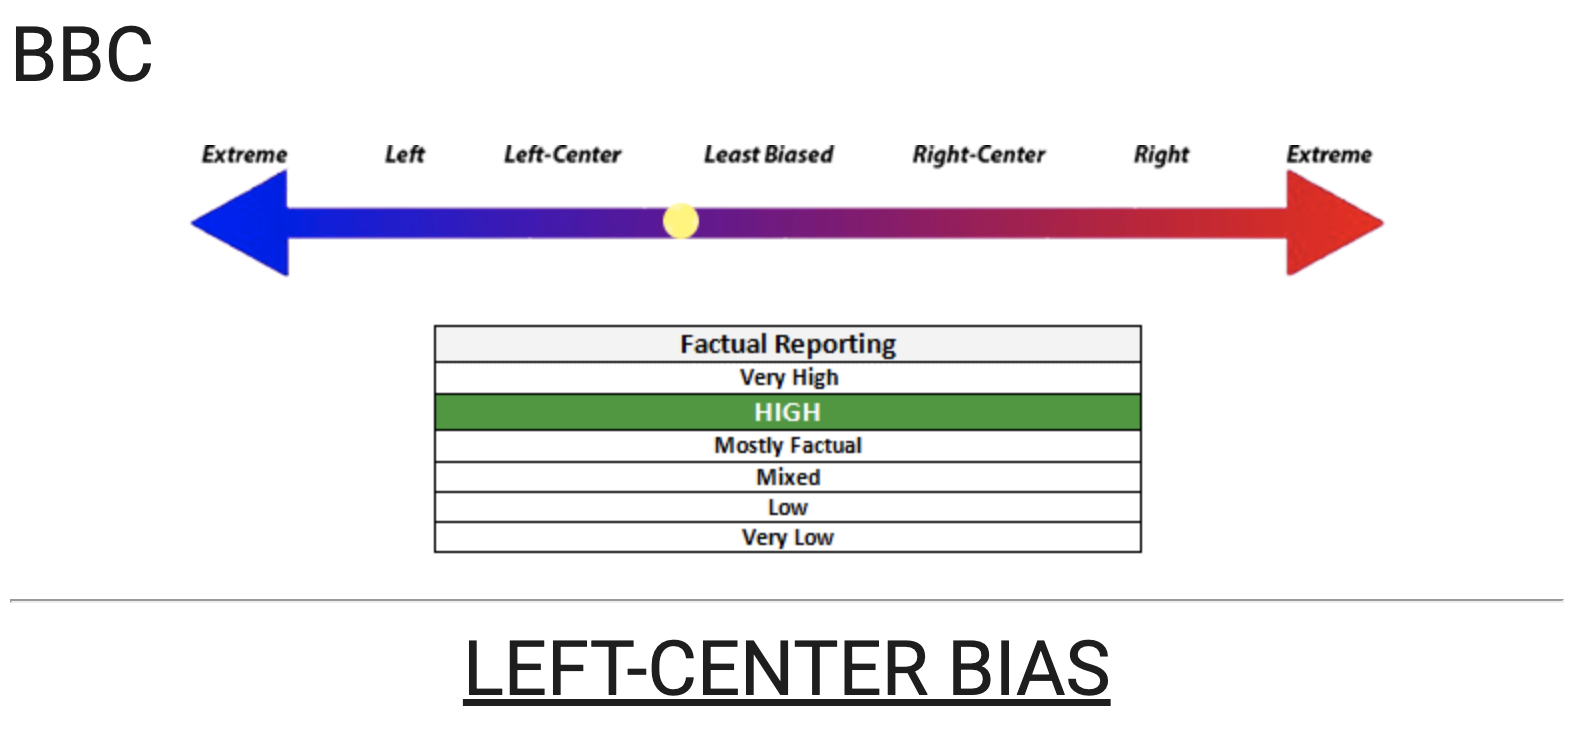
\includegraphics[width=\linewidth]{figures/mbfc_bbc.png}
    \caption{Example of rating from MBFC.}
    \label{fig:mbfc_bbc}
\end{figure}

We are interested in the leaning information, and they are grouped under 5 top-level categories:

\begin{itemize}
    \item \href{https://mediabiasfactcheck.com/left/}{Left Bias}: 351 sources;
    \item \href{https://mediabiasfactcheck.com/leftcenter/}{Left-Center Bias}: 904 sources;
    \item \href{https://mediabiasfactcheck.com/center/}{Least-Biased}: 1202 sources;
    \item \href{https://mediabiasfactcheck.com/right-center/}{Right-Center Bias}: 543 sources;
    \item \href{https://mediabiasfactcheck.com/right/}{Right Bias}: 252 sources.
\end{itemize}

Furthermore, this resource has other special categories, whose sources may also have a political leaning:

\begin{itemize}
    \item \href{https://mediabiasfactcheck.com/fake-news/}{Questionable Sources}: 1483 sources that may contain extreme bias, propaganda, conspiracies, poor sourcing, lack of transparency or fake news;
    \item \href{https://mediabiasfactcheck.com/conspiracy/}{Conspiracy-Pseudoscience}: 438 sources that usually publish unverifiable information lacking evidence;
    \item \href{https://mediabiasfactcheck.com/pro-science/}{Pro-Science}: 214 sources that are based on credible scientific sourcing;
    \item \href{https://mediabiasfactcheck.com/satire/}{Pro-Satire}: 149 sources that are clear that they are satire and do not try to deceive.
\end{itemize}

This dataset does not provide any articles, but it is used as reference by many other datasets in order to estimate the political leaning or the credibility of a news source.

We use this dataset in two different places in this chapter.
The first one, when experimenting with the political leaning classifier based on propaganda features, in Section~\ref{ssec:ps_prop_leaning_classifier}, as its leaning labels are used in the \texttt{NELA-GT18} dataset that we use as a secondary dataset to confirm our findings.
The second place where we use this dataset is in Section~\ref{ssec:ps_prop_leaning_imbalanced} to analyse the imbalance of the datasets across political leaning and we need its information to place news sources across the political spectrum.

\subsubsection{AllSides Dataset}
% stats updated 15/02/2023

Another very useful resource is AllSides\footnote{\url{https://www.allsides.com/}} which contains two different types of collections:

\begin{itemize}
    \item Sources collection: each source is annotated with its political leaning;
    \item Parallel news reports collection: \emph{Headline Roundups\texttrademark} made of 3 articles that discuss the same story, one from the Left, one from the Center and one from the Right.
\end{itemize}

\paragraph{Sources Collection}

As mentioned above, AllSides provides leaning annotations that differ from  the ones given only at the source-level.
As can be seen from the Media Bias Ratings published on their website,\footnote{\url{https://www.allsides.com/media-bias/ratings}} they have leaning ratings for different categories: Author (500), News Media (894), Think Tank / Policy Group (108), Reference (25) and Fact-Check (20).

This allows to know the leaning of specific articles written by authors even if they are published on news outlets with a different political leaning.


\paragraph{Headline Roundups\texttrademark}

The other collection that is very useful from AllSides is the Headline Roundups\texttrademark.\footnote{\url{https://www.allsides.com/headline-roundups}} In this section, the editors regularly publish a hand-curated set of stories. Each of them contains a brief textual introduction of how the story has been framed by the news coverage, and then displays three different articles coming from different political leanings

% is a platform that collects articles from different news sources providing a hand-curated set of stories where articles with opposing political bias are put together, with also a brief textual introduction of the framing differences.

\begin{figure}[!htbp]
    \centering
    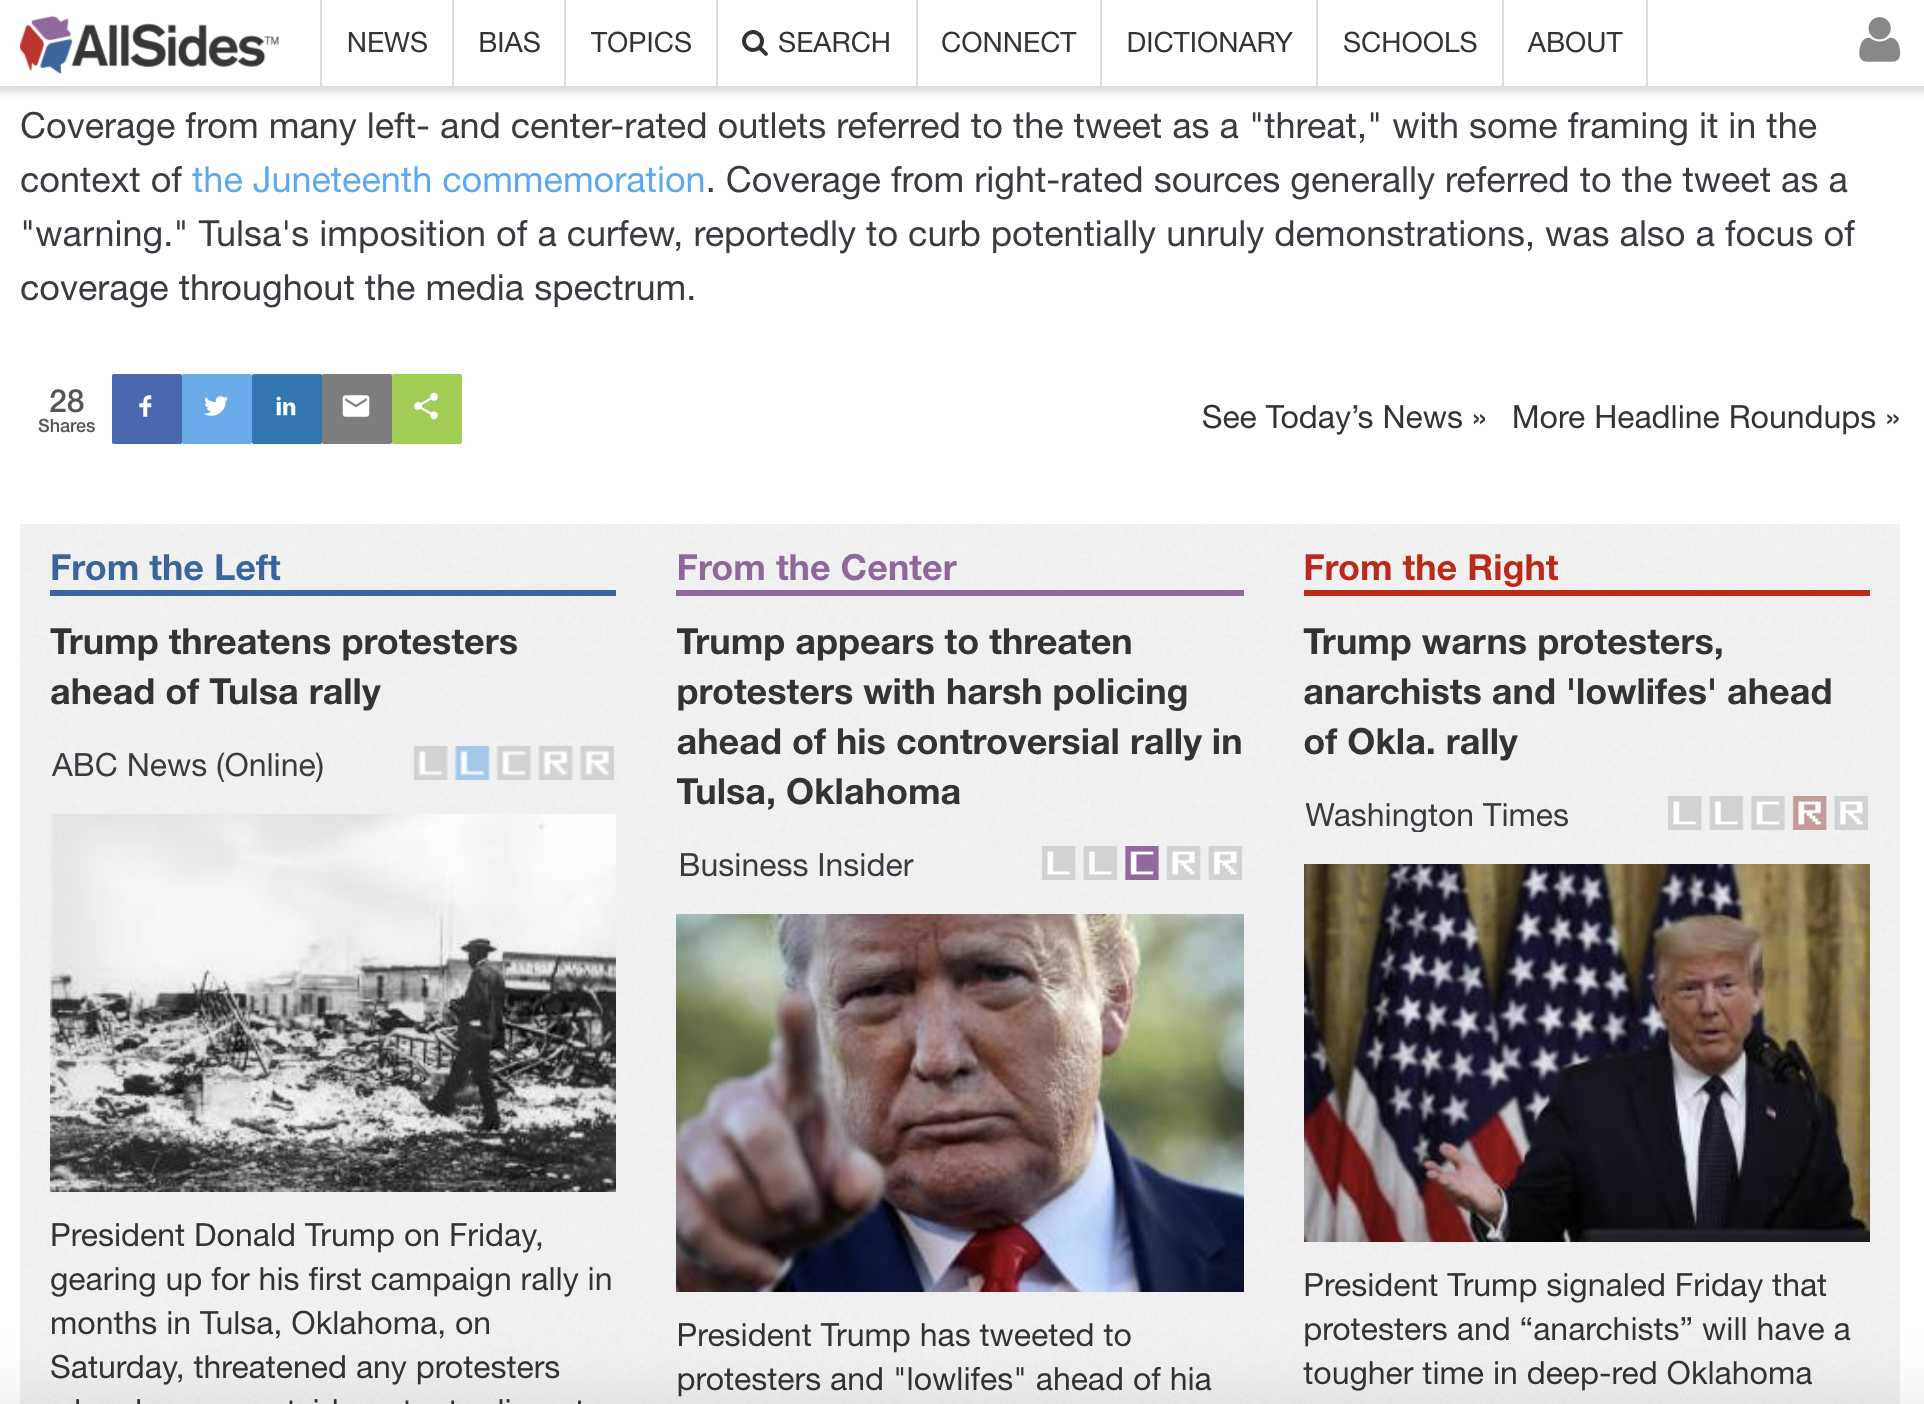
\includegraphics[width=\linewidth]{figures/allsides.png}
    \caption{Example of AllSides Headline Roundup.}
    \label{fig:allsides}
\end{figure}

In Figure~\ref{fig:allsides} we can see an example that displays how a source from the left, one from the centre and one from the right present the story of Trump tweeting about his rally in Tulsa.\footnote{\url{https://www.allsides.com/story/trump-tweets-about-protesters-ahead-saturday-tulsa-rally}}



% - allsides: human-created with interesting framing differences
% Another data source that we actively retrieve is AllSides which provides a curated set of ``headlines''\footnote{\url{https://www.allsides.com/story/admin}} where
The three articles with a different political leaning are put together and compared in their difference.
The curators describe how the story gets framed by the considered sources, using natural language.
This summary usually depicts which terms or themes are used. %\todoHA{sentence unclear}
% At the end of June, we have available 4764 headlines, with 13979 articles linked.
% Differently from Google Headlines which has different versions for each country, 
This data is US-focused being curated in the US and therefore has a limited scope. Also, the discussion of the differences is mainly focused on political issues, without giving much space to other topics.
% role of this specific data
% This data, although the description of the differences is not directly parseable, will be used to feed the user study and understand the role of comparing different sides.


% The work by~\citet{baly2020we} mentions that the annotations are defined on the article level. But in reality, we found that from the dataset all the articles from a specific source have the same leaning annotation. ??? TRUE? OR author level?

% STATS

This collection contains 7,766 headlines (as of 15/02/2023), for a total of 23,298 hyperlinks to articles.
%\todoHA{what's a link here?}
The oldest headlines were published in 2012.

%This is based on the observation 
By analysing the dataset, there are some articles (3.11\%) %(1,080 individual articles, 3.11\% on a total of 34737)
that have a leaning different from their source leaning.
This comes from the fact that some of the articles are annotated with the leaning of the author and not with the leaning of the news outlet, as we discussed before.
% \todoHA{and what does this lead to? which labels do you use?}
This is potentially leading to results that are more specific of the political leanings and less to the news sources. For example, a guest author that presents an opposite point of view with respect to the general alignment of the news outlet would not generate noise for the classifier, but would still produce valid annotated data samples.
Therefore, we use always the most detailed annotations available: political leaning of the author if available, and then as fallback the one of the news outlet.

%To clarify this point, we personally asked to the AllSides team about this discrepancy between article-level bias and source bias, and we understood that there are two types of annotation:
%\begin{itemize}
%   \item source-level annotation: in most of the cases, the articles are annotated with the bias of the media outlet
%   \item author-level annotation: sometimes, the articles are annotated with the bias of the specific writer, which can be different from the media bias\footnote{\url{https://www.allsides.com/media-bias/media-bias-ratings\#ratings}}
%\end{itemize}

%Therefore the 3.11\% is due to the author-level annotation. We want to underline that in this way, the annotation of the political leaning is not specifically assigned to the single article but instead it is assigned to the author. It is still a "distant supervision" in some extent.


This dataset has a characteristic that requires an additional data retrieval step in order to be used.
The text of the news articles is not directly provided, but it is made available by hyperlinks that reference the websites of the news outlets.
Therefore, to obtain the text, the hyperlinks need to be followed to scrape the body of the articles (plus cleaning step to remove non-related contents).


% For using this dataset directly, however, there is a limitation. The full text of the articles needs to be separately retrieved by connecting to the corresponding news outlets, and therefore the process of collecting and cleaning the data is not error-free.\todoHA{why introduce this here? how handled errors?}\todomargin{MM: to introduce the next dataset}

% We initially experimented with the data collected from this dataset, but we quickly found the limitation of applying custom data retrieval and also the problem of not having comparable results, as would happen with public and established datasets.\todoHA{rewrite clearly}
% \todoAWinline{I'm confused here. I'm not sure what you've put together yourself, and what you obtained elsewhere. Also, this is rather thin on the actual details of what you did to construct the datasets.}


\subsubsection{Baly dataset}
% \todoAW{Don't have more than three levels}

This dataset is derived from \emph{Allsides Headline Roundup\texttrademark}, as it was built in the work of~\citet{baly2020we} by downloading and cleaning from AllSides and from the respective news outlets all the articles (dataset including headlines until 21 July 2020).

The dataset therefore
% % FROM TTO2020
% The dataset we use is from~\citet{baly2020we}, and
consists of articles in English language from over 800 sources (majority from the US), labelled for their political leaning (Left, Centre or Right).
This dataset contains several attributes for each article: full text (collected from several news websites and cleaned), political leaning, topic, news source, and author name (attributes from AllSides).
% However, in our models and experiments, we only use the text of the articles to avoid bias associated with the other attributes.
The topic distribution of the articles is uniform across the political leanings, because the dataset comes from triples of articles, one from each political leaning, about the same issue.
% Authors of this paper publicly provide a dataset, collected from AllSides, where individual articles are labelled for their political leaning.
The dataset contains two pre-splitted folds for training and testing:
\begin{itemize}
    \item \texttt{Random}: where splits are randomly generated. Articles from the same media source may be contained both in the training and testing sets.
    \item \texttt{Media}; where the articles in the test set are from media sources that do not occur in the training set. %, which is more appropriate for article-based political leaning analysis. 
\end{itemize}

The Media split enables testing classifiers with less potential bias to previously seen sources, which instead happens with the Random split.
Otherwise, what could happen, is that deep-learning models can exploit this data as a shortcut~\citep{geirhos2020shortcut,baly2020we} to simply learn to recognise the style of the news source, and then from it to predict the leaning.
Instead of making the models exploit this information, the \texttt{media} split separates the sources and performs the evaluation on sources that are unseen during the training.
% Although the political-leaning of articles could sometimes be gauged by their sources, there are many examples where articles' political leaning differ from that of their sources, or the sources' leanings are not well known, or the sources themselves are unknown.
% Hence there is a need for such a detection to be independent of where an article came from.      
%and alignment.

\begin{table}[!htbp]
    \centering
    \begin{tabular}{r|c|c|c}
                      & train  & validation & test  \\
        \hline
        Paper media   & 22,969 & 5,098      & 1,200 \\
        GitHub media  & 26,590 & 2,356      & 1,300 \\
        \hline
        Paper random  & 26,828 & 6,709      & 1,200 \\
        GitHub random & 27,978 & 6,996      & 1,300
    \end{tabular}
    \caption{Differences between statistics from in~\citet{baly2020we} and GitHub.}
    \label{tab:baly_size}
\end{table}

Note that there is a discrepancy between the description of the dataset contained in its reference paper and the dataset made publicly available by the authors on GitHub.
The dataset described in ~\citet{baly2020we} contains 34,737 articles, whereas in GitHub\footnote{\url{https://github.com/ramybaly/Article-Bias-Prediction}} it has 37,554 articles (12,590 Left, 10,285 Centre, 13,399 Right). The details of this difference are shown in Table~\ref{tab:baly_size}, and have been reported to the authors.\footnote{\url{https://github.com/ramybaly/Article-Bias-Prediction/issues/4}}

\subsubsection{NELA-GT-2018}

This dataset, published in~\citet{DVN/ULHLCB_2019}, contains $713,534$ news articles coming from $194$ news sources (most frequent, in descending order: The Sun, The Telegraph, The Russophile, Sputnik, New York Post, The Independent, Drudge Report, Evening Standard, The Guardian, BBC, Instapundit, OANN, TruePundit, Daily Mirror, Daily Caller).

For each article, the available attributes are: publishing date, source, title and content.
Furthermore, for each source, there are many attributes that come from MBFC, AllSides, NewsGuard, Pew Research Center, Open Sources, BuzzFeed. Out of these many attributes, the one that refer to the political leaning are: MBFC, AllSides and BuzzFeed. Out of these three classifications, we find that in the majority of the cases, the labels agree and the only cases where they do not agree are between the Center label (by AllSides) and the Center-Left and Center-Right of MBFC. In other words, the systems only differ in the thresholds around the Center.
Instead, the labels from BuzzFeed cover a significantly lower number of sources, and they only have two values (Left and Right), without a Center category.

In Appendix~\ref{app:nela_processing} we present the processing that we have done on this dataset, to create balanced and unbalanced versions of both random and media splits for it.

\subsection{\statusgreen Models for Political Leaning Classification}
\label{ssec:ps_leaning_models}

% How it is computed

% Usual features

% State of the Art

% Problems: learning the source instead of learning L/R task
After having described the datasets, in this section we present the model that we have chosen from the literature (see Chapter~\ref{sec:lit_leaning}) for the task of \emph{political leaning classification}, and then we proceed to reproduce the baseline.

% FROM TTO2020

% Political leaning detection models have been produced for general media sources~\citep{budak} or for 
% specific political corpora such as congressional records~\citep{gentzkow}, political party websites~\citep{yan2017perils}, and political blogs~\citep{ahmed201}.  
% Others focused on inferring the political leaning of Twitter accounts~\citep{Cohen2013ClassifyingPO}, Facebook users~\citep{Bakshy1130}, politicians~\citep{thomas-etal-2006-get}, or political writers~\citep{iyyer-etal-2014-political}. 
% Various analysis methods were used in such studies, such as linguistic analysis \citep{gentzkow}, graph analysis \citep{chen2017opinion}, topic modelling \citep{ahmed201,Cohen2013ClassifyingPO}, support vector machines (SVM) \citep{Bakshy1130,thomas-etal-2006-get}, and neural networks \citep{iyyer-etal-2014-political,baly2020we}.

% We focus on detecting the political leaning of articles in a corpus of general news from a wide variety of sources. %, using a neural network approach fused with propaganda features. %\todo{description ok?} 

%often used supervised or unsupervised models applied to , or on opinion graph mining~\citep{thomas-etal-2006-get}.

%gentzkow - linguistic analysis 
%yan2017perils - regression models and neural networks
%budak - supervised learning and crowdsourcing
%ahmed - topic models
%Cohen2013ClassifyingPO - SVM and topic models
%bakshy support vector machine 
%thomas - svm
%iyyer - NN
%chen - SVM, LDA

%Most models use supervised or unsupervised machine learning algorithms, trained using source annotations or crowdsourced articles annotations  

%underlined that most of the approaches do not generalise well across domains. 
%As~\citet{yan2017perils} underline, three different classifiers trained on different types of texts (domains: congressional records~\citep{gentzkow}, political websites, wiki) result in lack of cross-domain generalisability (classifier trained on different domain struggles to find correct label on another domain, and mixing the training data reduces performance confusing the models).

In~\citet{baly2020we}, authors used a BERT-based model for predicting the political leaning of individual articles. The model takes as input the text of the article and produces one of three labels: Left/Centre/Right. The model is trained with a corpus from AllSides  (the previously described \texttt{Baly} dataset) which groups articles %with their political leaning 
according to the leaning of their source or of their author. %\todo{manually?}
%Authors found that 3.11\% of their 34737 articles from AllSides has a different leaning to that given to their sources (AllSides confirmed that this is due to using author-based leaning). 
%   \item source-level annotation: in most of the cases, the articles are annotated with the bias of the media outlet
%   \item author-level annotation: sometimes, the articles are annotated with the bias of the specific writer, which can be
% Similarly to \citet{baly2020we}, in this paper we also focus on classifying articles, regardless of their source and authorship. 


% Problem: learning the source instead of the political leaning
The main focus in~\citet{baly2020we} is to classify individual articles regardless of the source or author. This generalises better with unseen sources, and with cases were there is a difference between the political leaning of a particular article from that of its source.
% Authors found that 3.11\% of their 34737 articles from AllSides has a different leaning to the given to their sources (AllSides confirmed that this is due to using author-based leaning labels for some articles). 
% Other approaches focus on learning the media bias of a the source~\citep{baly2020written,biessmann2016automating}.



\subsubsection{\statusgreen Baseline Reproduction}
\label{ssec:ps_leaning_classifier}
% \todoAW{Very strange place for this section; I'd have expected it in the evaluation part.}
% \todomargin{Section 5.4 is already long enough. I am keeping this here, justifying it}

% Understanding the implicit political leaning of news articles could be seen as an indicative factor for identifying misinformation~\citep{spezzano2021s}. ???

% Our reproduction of classification from text (baselines):
% - TF-IDF
% - BERT


Having described in the previous subsections the relevant datasets and models for political leaning classification, and also being the next sections related to experiments that mix political leaning with persuasion (as described in the Introduction~\ref{sec:ps_intro}),
we present here the reproduction of the baseline of the political leaning classification that is used in the next sections.

Our baseline for article-level political leaning is~\citet{baly2020we}, which is the current state of the art for general purpose political leaning classification.
% Authors of this paper publicly provide a dataset, collected from AllSides, where individual articles are labelled for their political leaning.\footnote{\url{https://github.com/ramybaly/Article-Bias-Prediction}}
Since the source code for this work has not been released, we reproduced the architecture of the model by following the details provided by the authors. %in~\citet{baly2020we}. 
According to the details provided, we embed the articles in the dataset with a pre-trained BERT model (110M parameters, uncased\footnote{\url{https://huggingface.co/google/bert_uncased_L-12_H-768_A-12}}) and use the vectors from the second-to-last layer, as in \citet{baly2020we}. %\todo{unclear} %The model is made of a single dense layer (softmax activation function) which is trained and tested with the splits provided with the dataset in~\citet{baly2020we}.

\begin{table}[!htbp]
    \centering
    \scriptsize
    %\small
    % \resizebox{\textwidth}{!}{
    \begin{tabular}{l|rr|rr}
                                   & \multicolumn{2}{c}{Random} & \multicolumn{2}{c}{Media}                       \\
        Model                      & F1-Macro                   & Accuracy                  & F1-Macro & Accuracy \\
        \hline
        \texttt{Majority}          & 21.0286                    & 46.0769                   & 21.0286  & 46.0769  \\
        % \texttt{Baly-API} & 42.3355 & 43.8356 & 42.0523 & 43.6910 & 41.6863 & 41.7993 & & & & \\
        \texttt{Baly-baseline} (0) & 56.4447                    & 58.6153                   & 40.8647  & 46.2307  \\
        \texttt{Baly-paper} (*)    & 80.19                      & 79.83                     & 35.53    & 36.75    \\
    \end{tabular}
    % }
    \caption{Baselines results compared with~\citet{baly2020we}.}
    \label{tab:results_baselines_classifier}
\end{table}

Table~\ref{tab:results_baselines_classifier} shows the baseline results.
The row denoted with \texttt{Majority} represents a simple baseline that always provides in output the most common class. It has quite low results and is considered here just as a lower threshold for the values of the other models.
The row indicated with \texttt{Baly-paper} corresponds to the numbers reported in~\citet{baly2020we} (in their table~3, while \texttt{Baly-baseline} represents the results that we got from reproducing the experiments.

The difference is a significant drop for the random splits ($\sim80\% \rightarrow 56\%)$  while an increased value for the media splits ($\sim30\% \rightarrow 40\%$).
% Note, however, that the results we reproduced differ from those reported in their paper.
This quite big difference could be because of possible slight re-implementation discrepancies, and of the difference between the dataset reported in their paper and the one they shared on GitHub, as discussed previously in Section~\ref{ssec:ps_leaning_data}.%, which is likely to be due to later updates to the dataset. 
% Table~\ref{tab:results_baselines_classifier} shows the results we reproduced, which form our baseline (\texttt{Baly-baseline}). %For reference, we also include the results reported in the baseline model paper (\texttt{Baly-paper}).%, which are significant drop with the random splits while outperforming with the media splits.

Differences in the data and not sharing the implementation make it impossible to reproduce their baseline exactly.
Therefore, \texttt{Baly-baseline} represents our best effort in reproducing it.
In the next experiments, when we refer to the baseline
we mean the reproduction of the baseline as in \texttt{Baly-baseline}. Using the numbers from \texttt{Baly-paper} would not be fair, as the dataset used is different, and we want to exclude any other factors in the comparison of the results.


% TODO table from https://github.com/ramybaly/Article-Bias-Prediction/issues/4


% To test our three Research Questions (Section \ref{sec:intro}), we extend the model above with various propaganda-related features, and compare their outcomes to the baseline to see if and how adding propaganda features affect the classification results.\todo{move to Experiment Setup? and clarify different between when using your model alone vs combining with basline} 


% disclaimer
% Due to the small differences in the dataset and some possible differences also in the implementation of the baseline, we are not able to reproduce the results indicated as ``table 3'' of~\citet{baly2020we}. % We will substitute our implementation with the official baseline if and when its code will be shared. 

% The results of Table~\ref{tab:results_prop_features_classifier} show that the baseline we reproduced (\texttt{Baly-baseline}) achieves different results from the those reported in their paper (\texttt{Baly-paper}): 


%     \item \texttt{Baly-baseline}, being an emulation of what described in~\citet{baly2020we}, is still far from the 80\% results reported by the authors. 


% and we are still waiting for the official code to be released (containing the implementation of their model).


%are comparing this baseline with other similar models where we use features coming from the propaganda analysis (see next) and feeding them to a model with the same single dense layer.

% that we have are going to be tested by comparing the results obtained adding specific features to the reference model. 

% For complete comparability of the results, therefore, we need to use their dataset. However, since the dataset was released only in April 2021, the experiments are also considering our own data collection from AllSides.
% At the moment, we have their dataset available (articles annotated with L/C/R labels) but we still need to finish the automated annotation of propaganda techniques (each article annotated with the 18 techniques), through an API that has quite low rate limits. For this reason we present in the following sections still the results of our own datasets (we have the propaganda annotations of them because the rate limit has been introduced only recently).


% The first dataset, here denoted with \texttt{13k} because of its size, was collected from the Headlines\footnote{\url{https://www.allsides.com/story/admin}} which are groups of three articles, usually one from the left, one from the centre and one from the right (annotated at the author level).
% This results in a dataset made of 13k articles.

% Being this dataset much smaller than the reference one, we performed a second data collection which this time considers also articles that are annotated singularly, not in groups of three as before.\footnote{\url{https://www.allsides.com/unbiased-balanced-news}}.
% This second dataset collected instead has a size of 60k articles.
% The main difference with the first one is that the articles are not grouped in triples of Left/Center/Right. This results in the 60k dataset being much more imbalanced than the 13k (which still is a bit imbalanced because not exactly all the groups keep the balance).

% The third dataset is coming from~\citet{baly2020we} through the official GitHub repository \url{https://github.com/ramybaly/Article-Bias-Prediction}. We observe that there are some differences with what is stated in their paper, as can be seen in table~\ref{tab:baly_size}. What probably happened is that the authors kept collecting more articles.



% Now, by comparing the two different datasets collected with the dataset from~\citet{baly2020we}, Figure~\ref{fig:venn} shows that the 13k and Baly are mostly balanced subsets of the 60k.
% Although the URLs of the articles in the Baly dataset are a subset of the URLs of the articles in our datasets (13k and 60k), the texts of the articles do not match: the data cleaning of \texttt{Baly} is different and better than our data cleaning (e.g. removing non-article content), and having different texts makes the propaganda annotations differ slightly.

% The last dataset considered is derived from the 60k, by keeping it balanced between target labels. Since the smaller group (Center) has 11309 articles, we limited the articles from the Left and Right to contain 11309 articles too, through random selection. We will compare the results of the imbalanced 60k with the balanced 60k.

% TODO: only table or only histogramm
% \begin{figure}[!htb]
%     \centering
%     \includegraphics[width=\columnwidth]{figures/dataset_comparison.pdf}
%     \caption{Distribution of the three datasets across the political spectrum}
%     \label{fig:dataset_comparison}
% \end{figure}

% \begin{table}[!htb]
%     \centering
%     \begin{tabular}{l|r|r|r}
%         Dataset & \#Left & \#Center & \#Right \\
%         \hline
%         13k & 6058 & 2672 & 4408 \\
%         60k & 27457 & 12565 & 20441 \\
%         60k-balanced & 12565 & 12565 & 12565 \\
%     \end{tabular}
%     \caption{Distribution of the three datasets across the political spectrum}
%     \label{tab:dataset_comparison}
% \end{table}

% \begin{figure}[!htb]
%     \centering
%     \includegraphics[width=\columnwidth]{figures/venn.pdf}
%     \caption{Overlap between the three datasets}
%     \label{fig:venn}
% \end{figure}




% - source labels vs author labels?
% \\

% classifier comparison with theirs
% Since at the moment the results are shown from our datasets, the only way to compare with the baseline is to use the same model. For this, we are waiting for their implementation to be shared. In the meanwhile, we have tried to emulate the baseline, based on the description of the model given in~\citet{baly2020we}. We name this set of results with \texttt{Baly-baseline}. However, the results of this model are lower than the official results, so there have to be other differences other than the dataset size increased.
%     \item using a prediction endpoint of political leaning exposed by the same research group. We do not know if this endpoint is an implementation of the model described in~\citet{baly2020we} or not, the results will tell. We name this set of results with \texttt{Baly-API}.
% \end{itemize}
% Instead, for the second big issue of comparability (the model), we need to have their model implementation to compare our results. While the dataset was not shared with us, this was the only possible way to compare: feed our dataset to our models and theirs and compare fairly the scores. We found that their API exposes a political leaning prediction endpoint that accepts sending text and provides the probability of the article to belong to left/center/right. We don't know if this implementation is the one behind the paper (the prediction belongs to the same project at QCRI) but we assume it is.
% Therefore we sent all the articles that we have in our datasets to that endpoint and took the argmax of that prediction. The results collected with this method are annotated here with \texttt{Baly-API}.
% From the description given in their paper~\citep{baly2020we} we tried to reproduce locally the same model. We will observe how much this is the same with the results of \texttt{Baly-API}. These results are annotated with \texttt{Baly-baseline}.
% As soon as the implementation of the model will be shared by the authors, this confusion will be removed.
% \\


% \section{\statusgreen Persuasion and Political Leaning Classification} --> OLD 5.3 intro to 5.3.1, 5.3.2, 5.3.3 is now in 5.1 intro
% \label{sec:ps_prop_and_leaning}


\section{\statusgreen Persuasion Across the Political Spectrum}
\label{ssec:ps_prop_leaning_across}
% From Experiment 4.3: comparison of sentiment/propaganda across political leaning

Our first subquestion for this chapter is RQ3.1: \emph{How does persuasion vary across the political spectrum?}

To answer this question, we perform a comparison across the political leanings to see if we can identify major differences (for example, one leaning could contain more of one specific technique, or differentiate in the terms used).
For this reason, we perform the comparison by considering both the \emph{amount} of each persuasion technique, and the \emph{term frequencies}.

% - overall sentiment and propaganda across spectrum
%     - quantities
%     - terms
% - for each technique, what are the variations
%     - quantities
%     - terms


% Our hypothesis is that more extreme views will contain more persuasion (especially propaganda techniques).\todoAW{Slightly messy use of "hypothesis" here, given the way it's used in statistics. Maybe you want to say that you are investigating whether extreme views contain more persuasion. Then when you set up your experiment, the null hypothesis will be that there's no relationship between persuasion and extremity, and the alternative hypothesis is that extreme views contain more persuasion.}
We are investigating whether extreme views contain more persuasion.
This might be the case because stronger positions are characteristic of the extremes, while moderate and center views may express news in a more neutral way, less filled with persuasion.

\subsection{Experimental Setup}

% in short:
For this experiment, we want to see if there are some differences in the persuasion used by different political leanings, both considering the quantities of techniques and the terms used for the techniques.
% \todoAW{different amounts (which is what the previous para implies), or difference in the type of persuasion used?}
Therefore, we take a dataset, we run it through automated persuasion annotation tools, and then we compare the statistics across political leaning of the articles.

% dataset
The dataset used is \texttt{baly}~\citep{baly2020we}, as described previously in~\ref{ssec:ps_leaning_data}.
We take from it the text of the articles and the label for the leaning, expressed over 3 distinct values: Left, Center and Right.
%, Mixed, Not Rated. The first 5 values are properly placed across the spectrum, from left to right. The last values instead are for data that is not clearly aligned with one leaning.
It is important to note that the articles in this dataset are grouped in triples covering the same story, and this grouping makes the topic perfectly balanced across the dataset. For each article belonging to one leaning, there exist two other articles that belong to the other two leanings.
In this way, we do not need to consider the fact that some topics may naturally be more subject to persuasion (e.g. political issues) while other topics may be less (e.g. sports or technology, where the writing style could be less loaded).
Having this link between the articles in the dataset allows us to focus on the comparative results excluding the variable of the topic (for now, but we will introduce the topic as a variable in the next Chapter~\ref{chap:topics}).

% features extraction: sentiment/propaganda
From the text of each of the articles, we then extract the persuasion techniques (sentiment and propaganda, as in the previous Chapter~\ref{sec:lp_techniques}). This gives us for each document a set of words annotated with the corresponding technique. From these annotated words, we compute two features:
\begin{enumerate}
    \item word-based percentage of each technique;
    \item terms for each technique.
\end{enumerate}


% 1. Extraction of propaganda/sentiment
% Each article is analysed independently from the others, using the propaganda detection method and the sentiment lexicons.
% The percentages of words annotated with respect to the total number of words are computed for each article.

% 2. Grouping the percentages by political bias
We then consider the labels given by the dataset (Left, Center, Right), and we aggregate the average of word-based percentages (mean, quartiles, distribution). %This gives an idea of how much of the articles from each political side is detected as sentiment-related or propaganda-related.
We also aggregate the term distributions to compute the term relative importance (TF-IDF) to then understand if the Left, Center and Right are using different words to express their persuasion.

\subsection{Quantities of Persuasion Techniques across Leaning}

Here in this section we show the comparison across leanings of the \emph{quantities} of persuasion techniques.
First we compare the higher-level of propaganda vs sentiment, and then we break down the propaganda techniques, that provide a much more detailed picture.

\begin{figure}[!htbp]
    \centering
    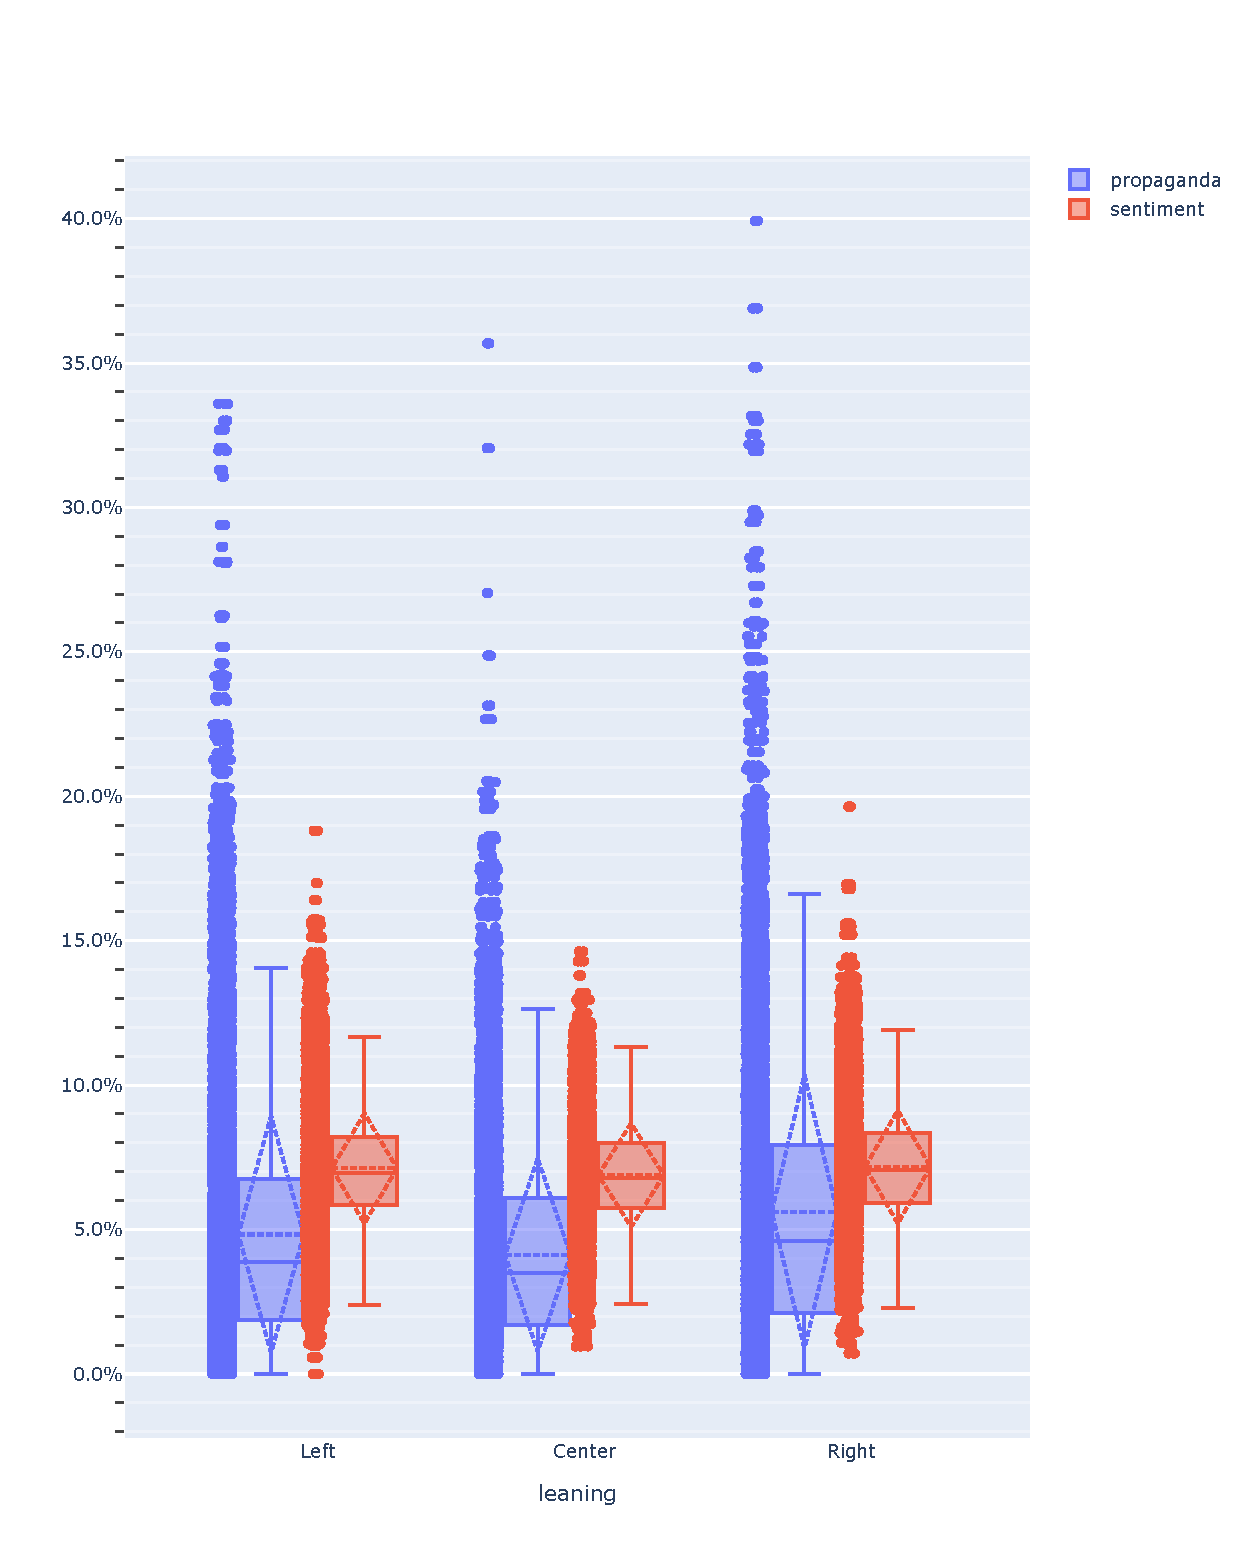
\includegraphics[width=\linewidth]{figures/prop_sent_tech_across_leaning_headlines_mod.pdf} % features_by_bias_box_cleaned_all.pdf
    \caption{Percentage of detected sentiment and propaganda across political leaning.}
    \label{fig:prop_sent_across_leaning}
\end{figure}
% \todoAWinline{Fig~\ref{fig:prop_sent_across_leaning} axis label?}

\subsubsection{Overall Quantity of Propaganda and Sentiment}
Figure~\ref{fig:prop_sent_across_leaning} is a representation which shows the distribution of the ratios computed.
On the vertical axis, the word-based percentage is represented. The boxes represent Q1 (25\% quartile) Q2 (median) and Q3 (75\% quartile). The diamond represents mean and standard deviation, while the whiskers are drawn within the 1.5 IQR value.
% (with data points on the left, and the boxplot with quartiles on the right)
We can see that for sentiment, we have very similar average values and distributions (median, Q1, Q3, mean).
For this reason, we conclude that sentiment is not a good indicator of the differences between political leanings. We cannot find any differences between left and right.

Instead, when we consider propaganda, we see that on the Right we have more words detected as propagandistic.
The Center has slightly fewer words detected in propaganda with respect to the other two leanings (mean values: Center=$4.1\%$, Left=$4.9\%$, Right=$5.6\%$).
This confirms our initial supposition that the center contains less propaganda than more polarised political leanings.

% We did a c

% From this plot we see that there are some very strange values (76\% of highlighted words in one article from the center). Looking at the details, this is an article from BBC which does not look so subjective. The problem is that from the full article, the scraping library only captured the sentence The statement says: ``It is an assault on UK sovereignty and any such use by a State party is a clear violation of the Chemical Weapons Convention and a breach of international law. It threatens the security of us all." which is annotated as almost everything propaganda. For other BBC articles, scraping manages to retrieve the full text without problems.

% There are also a lot of articles which have a percentage of 0\%. Looking at the distribution of the length of the documents, some documents, especially from some sources, have length=0 or a very short length (scraping the cookie disclaimer instead of the full article).
% For this reason a minimum length threshold has been set to cut out these problems: 150 tokens at least.

% This is the same plot, but with the filter on the minimum length.
% We can see that:
% The most annotated side is the Right
% The least annotated side is the Left
% Article from the Center do not contain less sentiment/propaganda (against assumption)
% There are fewer propaganda words than sentiment words

\subsubsection{Quantity of each Propaganda Technique}
% BREAKDOWN BY TECHNIQUE
We then analyse more in detail the breakdown by specific propaganda technique. For this, we keep separated the word-based percentages for each technique.
Our aim is to see whether some techniques are used more in one specific leaning than in the others.


\begin{figure}[!htbp]
    \centering
    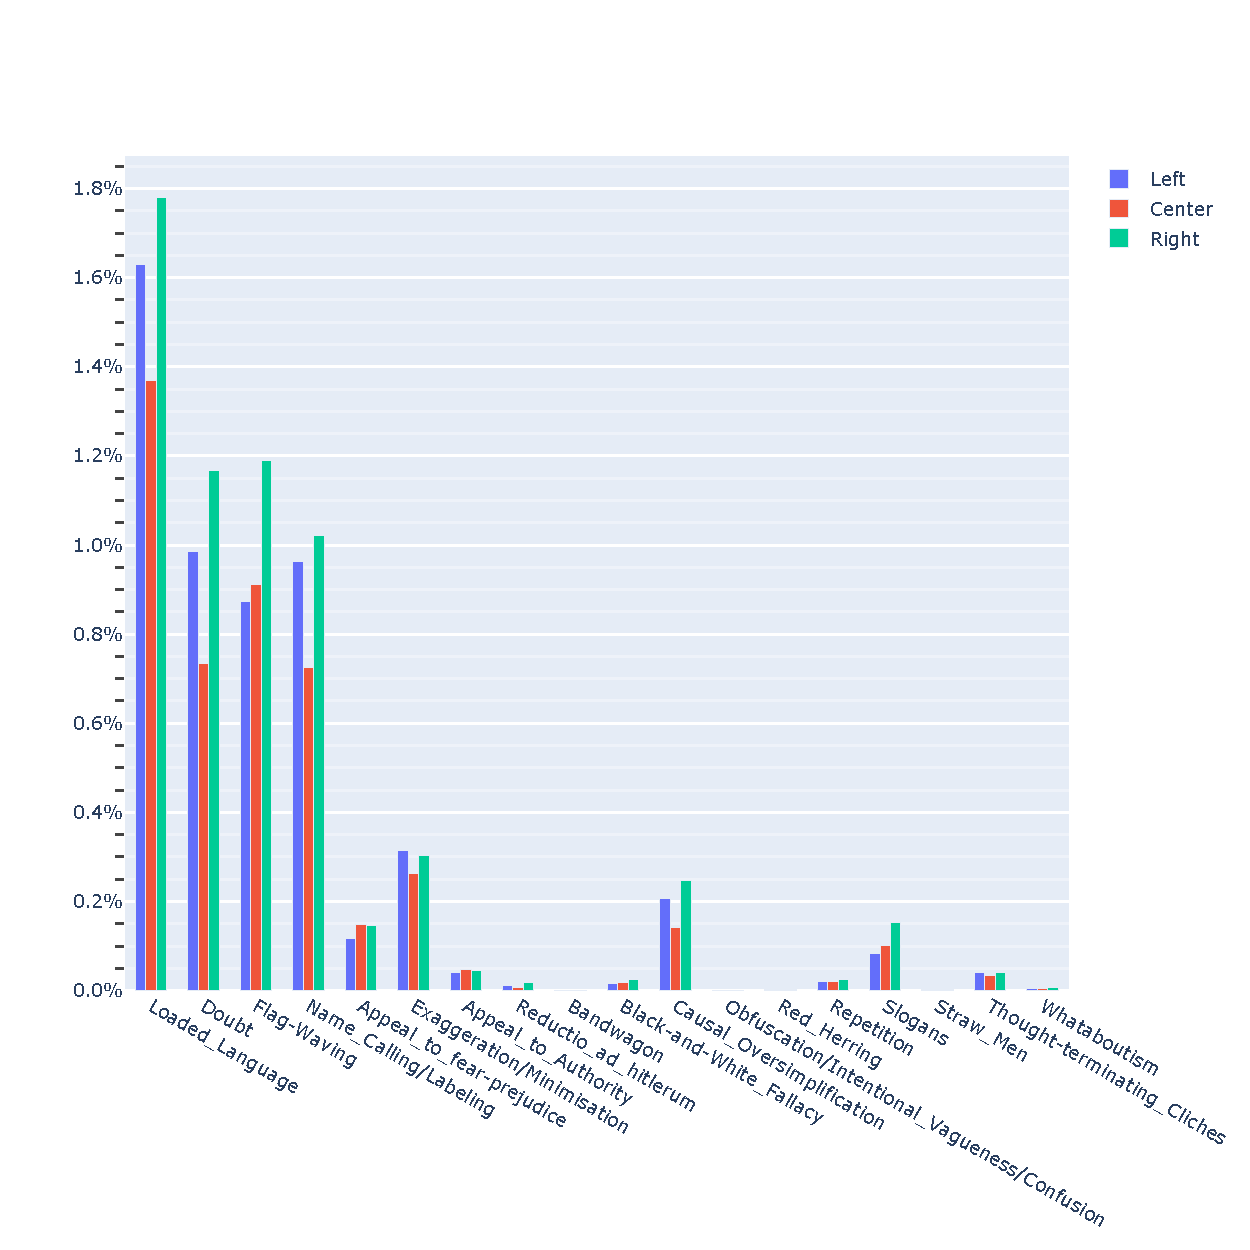
\includegraphics[trim={0 0 0 2cm},clip,width=\linewidth]{figures/prop_tech_detail_across_leaning_baly.pdf}
    \caption{Breakdown of propaganda techniques by political leaning.}
    \label{fig:prop_tech_details_across_leaning}
\end{figure}
% \todo{Fig~\ref{fig:prop_tech_details_across_leaning} Would it be better to show also std deviation or other distribution info like in the previous plot? Or too cluttered?}

Figure~\ref{fig:prop_tech_details_across_leaning} shows on the vertical axis the different propaganda techniques, and each colour represents a different political leaning. The vertical axis represents the mean word-based percentage of the specific propaganda technique for the considered leaning.
With this plot we can compare the techniques across the leanings.

First of all, we notice that the most common propaganda techniques are \texttt{Loaded\_Language}, \texttt{Doubt}, \texttt{Flag-Waving} and \texttt{Name\_Calling/Labeling}.
The articles in the dataset contain on average $1.5$ loaded terms every $100$ words.

% shape analysis
We can see different types of patterns in this plot, which are shown with different shapes over the leanings.
% U-shape
The first one, that we call \emph{U-shape}, happens when the bars of the Left and Right are higher than the bar of the Center. This means that what is represented is polarised on the extremes of the political spectrum.
A good example of this type is the \texttt{Loaded\_Language}, where the Center is using this technique on $1.38\%$ of the words, while Left and Right are using it considerably more.
The same happens with \texttt{Doubt}, \texttt{Name\_Calling/Labeling}, \texttt{Exaggeration/Minimisation}, \texttt{Causal\_Oversimplification}.
These techniques are used by more extreme articles and are giving the general trend that we observed in the previous Figure~\ref{fig:prop_sent_across_leaning}: the center is more moderate and uses propaganda less.

% triangular shape
A second pattern that we notice, is the \emph{triangular shape}. In this shape, the quantities of the technique considered increase (\emph{triangular Right}) or decrease (\emph{triangular Left}) monotonically when going from Left to Right leaning.
This behaviour means that the technique analysed is inherent of a specific extreme of the political leaning spectrum, and constantly decreases when moving to the other side.
It is not surprising that \texttt{Flag-Waving} presents this behaviour, where it is way more detected in Right-leaning articles with respect to Center and even more with Left. This technique is conceptually linked with the principles of nationality, and the strong nationalism is usually associated with Right-leaning political stance.
The same pattern occurs with \texttt{Slogans}. We can link this with the abundance of left-leaning slogans in the recent date range of the dataset for the Trump re-election campaign~\citep{jiang2020political}.

% Reversed U
Another pattern that we see, is the opposite of the first one: \emph{reversed-U shape}. This is characterised by a higher use in the Center than in the extremes.
We can see this pattern with the techniques \texttt{Appeal\_to\_fear-prejudice} and \texttt{Appeal\_to\_authority}. While for the first one, it is imbalanced (highest value center, then Right and then quite less Left), in the second case this is more balanced (Left and Right have similar values).
These techniques may be used with different intents: both for agitate the crowds with strong sentiment (fear and prejudice) or oppositely to moderate and provide as evidences the opinions of the experts (appeal to authority)~\citep{walton2010appeal}. It may be the case that, especially \texttt{Appeal\_to\_authority}, results to be appearing more in the center because of this reason.

\subsection{Propaganda Terms across Leaning}
We then move to the term analysis, to see if we can find any differences in the specific terms used by each leaning.

% One of the first thoughts when comparing terms from different groups, is WordClouds.
% They are a simple and qualitative way to compare distributions of terms.
% Therefore, we computed the WordClouds for the three leanings (Left, Center and Right).


% \begin{figure*}[!htb]
%      \centering
%      \begin{subfigure}[b]{0.3\textwidth}
%          \centering
%          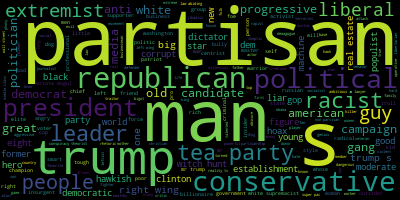
\includegraphics[width=\textwidth]{figures/baly_wordclouds_Name_Calling,Labeling_Left.png}
%          \caption{Left}
%          \label{fig:wc_loaded_left}
%      \end{subfigure}
%      \hfill
%      \begin{subfigure}[b]{0.3\textwidth}
%          \centering
%          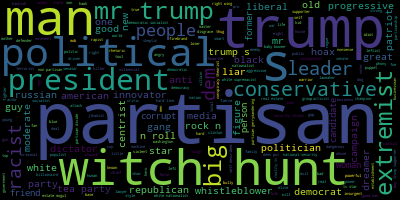
\includegraphics[width=\textwidth]{figures/baly_wordclouds_Name_Calling,Labeling_Center.png}
%          \caption{Center}
%          \label{fig:wc_loaded_center}
%      \end{subfigure}
%      \hfill
%      \begin{subfigure}[b]{0.3\textwidth}
%          \centering
%          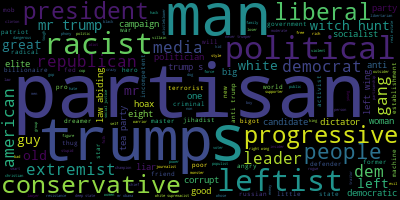
\includegraphics[width=\textwidth]{figures/baly_wordclouds_Name_Calling,Labeling_Right.png}
%          \caption{Right}
%          \label{fig:wc_loaded_right}
%      \end{subfigure}
%         \caption{WordClouds from words belonging to the \texttt{Name\_Calling} propaganda technique}
%         \label{fig:wc_name_calling}
% \end{figure*}

% % Qualitative term analysis done on the words belonging to the different political leanings in our dataset. 
% \todoHAinline{You can't conduce anything from wordclouds. Think of better analysis techniques.}
% \todo{It was an example to then motivate the choice of TF-IDF analysis}
% As Figure~\ref{fig:wc_name_calling} shows, 
By doing a simple ranking of the most important terms for each leaning, we can see some differences in some of the propaganda techniques. For example, considering the \texttt{Name\_Calling} technique:
media sources from the Left appear to frequently use ``republican'' and ``conservative'', while in the Right we can see some unique terms such as ``leftist'' and ``progressive''. Some words are equally used, possibly for different meanings, such as ``partisan''.
Although these differences, the most repeated word from all the leanings is the word ``partisan'' which is used as a wildcard and probably is intended with different meanings.
But the effect is that most of the terms are repeated in all the leanings, and therefore we have to rely on a better concept than simply counting the term occurrences.

% WHY JUST TERM COUNTING IS NOT ENOUGH: example from wordclouds. Similar terms, just a few are unique of the leaning. The importance of comparing distributions and IDF
This is why we use the concept of relative term importance, %from TF-IDF
% We rely on the concept of term importance, 
as defined by the TF-IDF model: the importance of a term is directly proportional to how many times it appears in the considered document (Term Frequency) and inversely proportional to the number of times it appears in the whole corpus (Inverse Document Frequency).

Here, since we want to understand the relative importance of terms between political leanings, we consider as documents the concatenation of all the selected terms (from propaganda analysis) from all the articles coming from a certain leaning. In other words, we have a corpus made of 3 documents (one for Left, one for Center, one for Right).

We perform this analysis first with all the propaganda techniques together, and secondly by considering each technique separately.

\subsubsection{Propaganda Terms Analysis}
% TERM ANALYSIS OVERALL
For the term importance across all the propaganda techniques, we process each article and select the detected words of propaganda that belong to any of the 18 techniques. Then we collect all these words in 3 buckets, one for each leaning.
We apply on these 3 groups the standard TF-IDF as provided by the \texttt{gensim} library. %(applied on lemmatised words).
This produces a matrix of weights with a shape of $[n_{features}, 3]$ (feature size x number of classes), together with the features names.
Afterwards, we
computed for each term the difference of the TF-IDF scores between Right and Left.
These values then are used in absolute value to rank the features (words) that differ the most.
This ranking index formulation is therefore:

% absolute value of the difference between the TF-IDF scores of the terms between left and right
$$ i_w = | T_{w,R} - T_{w,L} | $$
where $T_{w,R}$ and $T_{w,L}$ are the TF-IDF scores of the word $w$ respectively in the Right and Left.
Therefore, to identify the features that differ the most between the leanings, we just consider the index just described and we rank the features names accordingly.
% ranked the features based on decreasing this value, as a sorting index computed for each feature.
In this way, we get as first ones the features whose values have the maximal difference.
% These features have high value for the leaning they are mostly occurring in, and lower values for the leaning where they do not appear very frequently.
We can then say that these terms are the most distinguishable propaganda terms across the political spectrum.

\begin{figure}[!htbp]
    \centering
    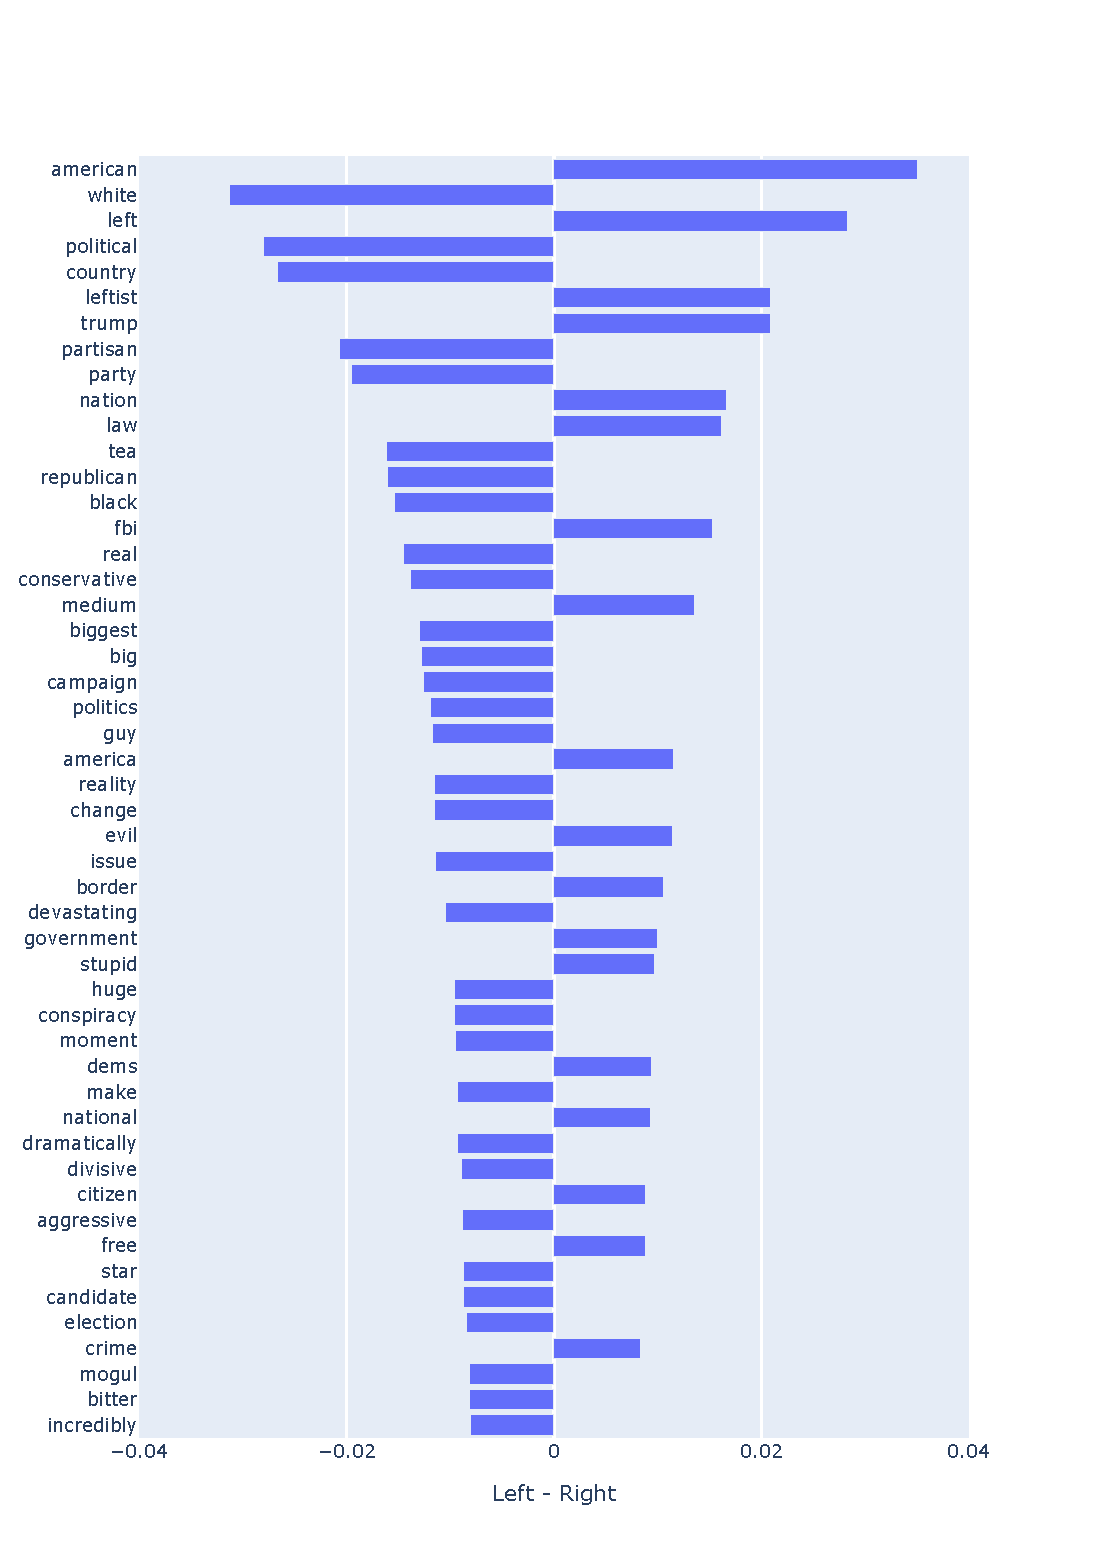
\includegraphics[trim={0 0 0 2cm},clip,width=\linewidth]{figures/baly_prop_tech_words_all_across_leaning_simple.pdf}
    \caption{Most distinguishable Propaganda terms across political leaning.}
    \label{fig:baly_prop_tech_words_all_across_leaning}
\end{figure}

Figure~\ref{fig:baly_prop_tech_words_all_across_leaning} shows the top 50 features (words) that have the highest difference between Left and Right TF-IDF scores.
On the horizontal axis, we can see the relative value of the difference on the Left-Right dimension.
% We did not remove stopwords because we are only dealing with some fragments of sentences that have been detected as propagandistic. For this reason the plot is showing some stopwords (e.g., ``a", ``of", ``the").\todoHA{Unclear why this stops you from removing stop-words}
From this plot we can recognise some propaganda terms.
For example ``american", ``left", ``leftist", ``nation", ``law" and ``border" that are more important for the Right. From~\citet{seargeant2020art} we know that the Right is using statements
% like ``we the people" which is a Right-leaning expression of populism.
that relate more with the identity  (american and nation) and protection  (law and border) of the country.
We also see the terms used to indicate the political opponents: ``leftist" and ``left".
Instead in the Left, we see terms such as ``white" and ``black" (emerging from articles about discrimination), ``partisan" ``republican" and ``conservative" (propaganda talking about the political opponents).
% Then we notice some terms that are more related to the center: ``country", ``trump", ``nation", ``partisan", ``whistleblower", ``great".

\subsubsection{Propaganda Terms by Technique}
% TERM ANALYSIS PER TECHNIQUE
However, from this analysis, it is not clear how the terms found relate to the specific propaganda techniques. For this reason, we decide to perform again this analysis, but for each propaganda technique separately.
This means that we build the term frequencies for each of the 18 techniques, by collecting the terms that have been used in the specific technique by each leaning, and then building the TF-IDF feature separately and sorting again by the $(max - min)$ criterion.


\begin{table}[!htbp]
    % \Rotatebox{90}{%
    \resizebox{\textwidth}{!}{
        \centering
        \begin{tabular}{p{0.30\textwidth}|p{0.40\textwidth}|p{0.40\textwidth}|p{0.40\textwidth}}
            technique                                                & Left                                                                          & Center                                                                                                                                  & Right                                                                                \\
            \hline
            \texttt{Loaded\_Language}                                & in, that, into, self, devastating, hell                                       & balk, more, very, whistleblower, hit, expose, batten, out, badgering, divisive, blast, circus, dramatic, chaos, severe                  & evil, blasted                                                                        \\
            \hline
            \texttt{Doubt}                                           & just                                                                          & trump, inadequate, transparency, grapple, will                                                                                          & why, FBI, if                                                                         \\
            \hline
            \texttt{Flag-Waving}                                     & America, \textbf{white}, \textbf{black}, \textbf{life}, \textbf{society}      & democracy, state, security, family, value                                                                                               & \textbf{people}, \textbf{we}, \textbf{freedom}, \textbf{law}, \textbf{liberty}       \\
            \hline
            \texttt{Name\_Calling/ Labeling}                         & party, \textbf{republican}, \textbf{right}, \textbf{conservative}, wing, real & \textbf{partisan}, trump, witch, hunt, dems, whistleblower, innovator, dreamer, \textbf{centrist}, president, \textbf{democratic}, hoax & \textbf{leftist}, racist, hating, law, \textbf{liberal}, \textbf{progressive}        \\
            \hline
            \texttt{Appeal\_to\_fear- prejudice}                     & \textbf{threat}, \textbf{climate}, difficult, death, die, disproportionate    & risk, backfire, credible, dangerous, confidence                                                                                         & all, \textbf{destroy}, \textbf{attack}, fight, economically, racism, \textbf{invade} \\
            \hline
            \texttt{Exaggeration/ Minimisation}                      & best, more, incredible, impossible, biggest, could, dramatically              & history, deadliest, big, unprecedented, life, degradation                                                                               & worst, absolutely, great, ever                                                       \\
            \hline
            \texttt{Appeal\_to\_Authority}                           & medium, wisdom, \textbf{news}, know                                           & transparent, \textbf{intelligence}, official                                                                                            & \textbf{note}, lie, open, \textbf{written}, accurate, fair, reflect                  \\
            \hline
            \texttt{Reductio\_ad\_ hitlerum}                         & Stalinist, communism, partisan,                                               & gestapo, nazi, eagle, religion, blame,                                                                                                  & hitler, Donald, tactic, propaganda, resurgent, science, death, gay                   \\
            \hline
            \texttt{Bandwagon}                                       & find, common                                                                  & say                                                                                                                                     & taken, some, leave, future                                                           \\
            \hline
            \texttt{Black-and-White\_ Fallacy}                       & evolution, bible, proof, fall,                                                & impeachable, wall, good, strength, punch, military, justice, democratic, deal                                                           & my, live, change, amendment, senate                                                  \\
            \hline
            \texttt{Causal\_ Oversimplification}                     & plot, think                                                                   & all, say, \textbf{reality}, reason, political                                                                                           & member, \textbf{leftist}, life, left                                                 \\
            \hline
            \texttt{Obfuscation/ Intentional\_ Vagueness/ Confusion} & suggest, wrong, impossible, guide, evil, efficacy, anything                   & power, right, answer, excuse, truth, simply                                                                                             & wing, meaning, rule, master, magic, fiction                                          \\
            \hline
            \texttt{Red\_Herring}                                    & love, pay, believe, anymore, like                                             &                                                                                                                                         & life, think, family, adulterous, America, republican, statement                      \\
            \hline
            \texttt{Repetition}                                      & jealous, blind, ObamaCare, bully, poison, lie                                 & more, temple, satanic, breathe                                                                                                          & trump, obama, abiding, careless, law, pray, rigged, extremely                        \\
            \hline
            \texttt{Slogans}                                         & survival, fight, \textbf{matter}, \textbf{life}, face, \textbf{lives}         & \textbf{America}, first, \textbf{great}, win, \textbf{make}, anchor, hero                                                               & learn, amid, hearing, over, call, tax, race                                          \\
            \hline
            \texttt{Straw\_Men}                                      & read, vote, opposition, trump                                                 & love, rule, poll                                                                                                                        & lie, news, god, want                                                                 \\
            \hline
            \texttt{Thought-terminating\_ Cliches}                   & give, follow, lie                                                             & wasting, time, drama                                                                                                                    & enough, break, evidence                                                              \\
            \hline
            \texttt{Whataboutism}                                    & control, prison,                                                              & point, system, news, real, democrat, care                                                                                               & apartheid, people, law, American, make, worse, contain                               \\
        \end{tabular}
    }
    \caption{Most recognisable propaganda terms for each technique across leaning.}
    \label{tab:prop_words_by_technique_and_leaning}
\end{table}

With this method, we collect the most important words for each technique and leaning in Table~\ref{tab:prop_words_by_technique_and_leaning}.
%
As we can see, for each propaganda techniques there are different terms that are more or less important for each leaning.
While for some of these techniques, the terms shown by our analysis may not be very straightforward to interpret,
%are not very talkative,\todoHA{?} we can see
in some other cases the results are quite meaningful.
For example, in the \texttt{Name\_Calling/Labeling} technique we can see how the different political leanings address each others: the Right addresses the Left with the term \emph{leftist}, \emph{liberal} and \emph{progressive} and never with \emph{democrats} (term used instead by the Center). Instead, the Left addresses the Right with \emph{republican}, \emph{right} and \emph{conservative}.

Or for the \texttt{Flag-Waving} technique, we see how \emph{we the people} emerges from the Right, while the Left is more about \emph{white/black} and \emph{life/society}.
Also in the \texttt{Appeal\_to\_fear-prejudice}, we can see how thematically the Right is more recognisable for terms related to invasion/attack/destruction, while the Left emerges uniquely with \emph{climate}.
For the \texttt{Appeal\_to\_Authority}, the left has more use of the term \emph{news}, the Center instead with \emph{intelligence} and the Right with terms related to writing (\emph{written/note}).
Still in the \texttt{Slogans} technique, the center outlets emerges with the repetition of \emph{make America great again}, while the Left is repeating more the slogan \emph{Black lives matter}.

\subsection{Findings and Discussion}

The results from this experiment show that propaganda is used quite differently across the political leaning.
% We see significant\todoHA{Were the differences significant?}\todoAW{Very loaded word. Have you done a significance test?}
We are able to detect
differences both on aspects related to the amount of propaganda used, and on aspects related to the specific terms used.

% Quantities findings,  motivations and implications
Related to the quantities, we have the overall finding that we are detecting more propaganda on the articles coming from Right-leaning.
Left-leaning has slightly less propaganda and the Center has even less.
This relates with our expectation that propaganda is used more to express opinions on the extremes of the political spectrum, while in the center the discussions are kept a bit more neutral.
%\todoHA{What about the bias of the detection method to right propaganda?}
But as well, this could be a consequence of the detection method, that may be biased to recognise more easily propaganda from Right-leaning articles.
At the same time, we see that the sentiment analysis is showing similar distributions across the political leanings.
%\todoAW{Again, have you done a significance test?}

To go more in detail, we differentiated our analysis by considering the different propaganda techniques separately, and we have been able to find techniques that follow the general trend (\emph{U-shape}) across the leaning: \texttt{Loaded\_Language}, \texttt{Name\_Calling/Labeling}, \texttt{Exaggeration/Minimisation} and \texttt{Causal\_Oversimplification} with their polarising characteristics (extremes more, center less). Other techniques instead are more proper of one of the two leanings (\emph{triangular shape}): \texttt{Flag-Waving} and \texttt{Slogans} mostly on the Right.


% Terms findings, motivations and implications
Instead, for the term analysis, we were able for some techniques to interpret the differences in the term importances by linking them to an understanding of the context of the dataset. For example, in \texttt{Flag-Waving} we recognised \textit{we the people} emerging from the Right-wing populism, or words from very frequently used slogans in the \texttt{Slogans} technique.
Recognising these features in the text can give a higher probability of belonging to one leaning than to the others.

% discussion
The quantity analysis provided quite useful insights into the preferred techniques from news sources coming from different political leanings. Instead, the term analysis provided us with important terms that occur more in one leaning than in the others.
We have a much better understanding of how propaganda differs across the political spectrum.

% limitations
However, we have some limitations. By inspecting the samples, we observed in many cases that only parts of a technique were detected (boundaries not correctly captured, excluding terms that could be very useful for our term analysis).
% \todoHA{Examples?}
This is the own limitation of the current detection technique, which we took as it is and whose improvement is out of the scope of this thesis.

% link to next chapter
Furthermore, we would need to capture a bit more around the context of the propaganda techniques in order to understand what is their intent. We think that by analysing the topics of the articles more in details we could understand better the targets of propaganda and how propaganda is used as a mean to persuade in a certain direction about the topics. We will investigate the topics in the next Chapter~\ref{chap:topics}.

% link to next experiment
As the last limitation, we extracted these insights, but we do not know to what extent they reflect in an immediate and definitive indication of the leaning of the articles.
The weightings of the TF-IDF show, in many cases, very similar scores. Therefore, it is unclear for now how easy or hard it would be to use these features to automatically recognise the leaning of one article. %(more in the next Subsection~\ref{ssec:ps_prop_leaning_classifier})
% it is not clear whether these features can be used to automatically differentiate between the propaganda of the left and the one from the right.
We experiment in this direction with the following Section~\ref{ssec:ps_prop_leaning_classifier}.


% \subsubsection{REMOVE: this subsubsection is about removing propaganda to increase similarity across leanings}
% \todo{This is describing another dubious experiment: removing propaganda to increase similarity of articles that refer to the same story. Instead here I want to talk about the analysis of propaganda across spectrum}
% Instead of measuring the effect of removing the “framing” pieces on clustering algorithms, here we want to observe what is the effect on document similarity between different sources.
% Given articles from the left/center/right, we want to compare if there is a change in similarity when we remove sentiment and propaganda terms (e.g., articles are more similar than before).
% Hypothesis
% When removing propaganda/sentiment some political sides will be more similar to others. This is because the different parts are related to the propaganda/sentiment which is an added layer on top of the facts described.

% 1. Extraction of propaganda/sentiment
% Each article is analysed independently from the others, using the propaganda detection method and the sentiment lexicons.
% The percentages of words annotated with respect to the total number of words are computed for each article.
% 2. Grouping the percentages by political bias
% Considering the labels given by AllSides (left, lean-left, center, lean-right, right, mixed, not-rated), the average of sentiment-words-ratio, propaganda-words-ratio and both-ratio are computed. This gives an idea of how much of the articles from each political side is detected as sentiment-related or propaganda-related.

% % \begin{figure}[!htbp]
% %     \centering
% %     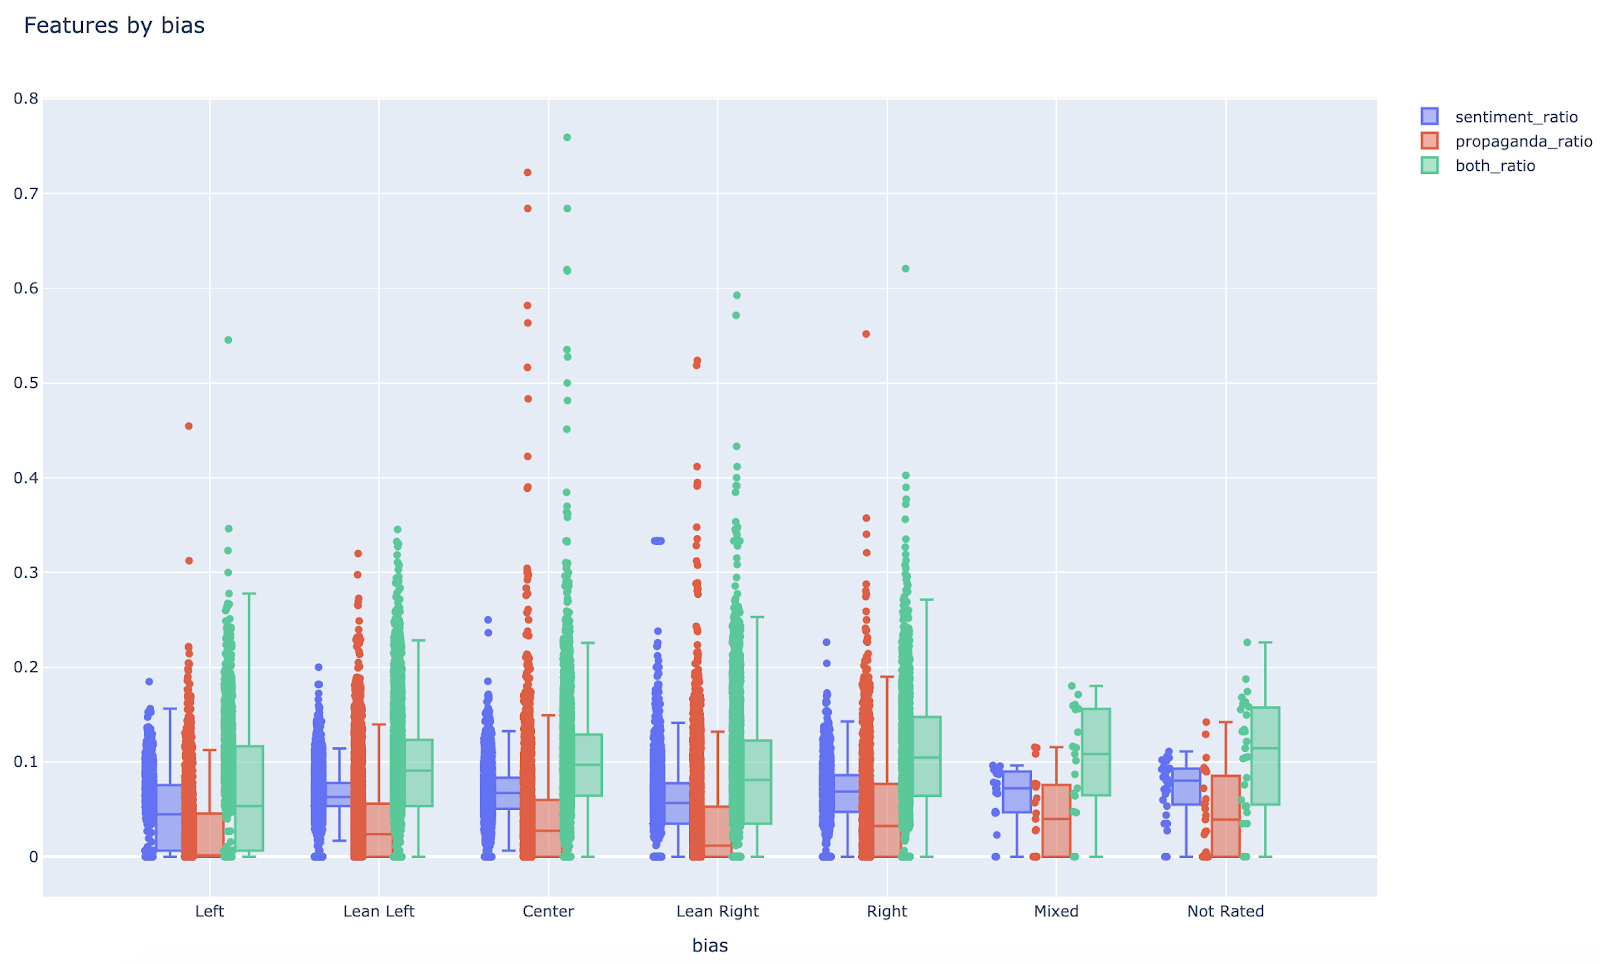
\includegraphics[width=\linewidth]{figures/4.3_prop_sent_across_leaning.png}
% %     \caption{Comparison of the detected sentiment and propaganda across the political leaning}
% %     \label{fig:prop_sent_across_leaning}
% % \end{figure}
% % \todo{Replace Figure~\ref{fig:prop_sent_across_leaning} with the one cleaned up, next in google docs}

% This plot in Figure~\ref{fig:prop_sent_across_leaning} is a quartile representation (with data points on the left of the boxes) which shows the distribution of the ratios computed. We can see that the average value (the line in the middle of the box) of “both\_ratio” is the highest for the “Right” side.
% From this plot we see that there are some very strange values (76\% of highlighted words in one article from the center). Looking at the details, this is an article from BBC which does not look so subjective. The problem is that from the full article, the scraping library only captured the sentence The statement says: ``It is an assault on UK sovereignty and any such use by a State party is a clear violation of the Chemical Weapons Convention and a breach of international law. It threatens the security of us all." which is annotated as almost everything propaganda. For other BBC articles, scraping manages to retrieve the full text without problems.

% There are also a lot of articles which have a percentage of 0\%. Looking at the distribution of the length of the documents, some documents, especially from some sources, have length=0 or a very short length (scraping the cookie disclaimer instead of the full article).
% For this reason a minimum length threshold has been set to cut out these problems: 150 tokens at least.

% This is the same plot, but with the filter on the minimum length.
% We can see that:
% The most annotated side is the Right
% The least annotated side is the Left
% Article from the Center do not contain less sentiment/propaganda (against assumption)
% There are less propaganda words than sentiment words



% 3. Creation of modified documents without the sentiment/propaganda parts
% As in the previous experiment (clustering), for each document other three documents have been created:
% Without propaganda words
% Without sentiment words
% Without propaganda and sentiment words
% Each document is embedded with two different methods:
% Universal Sentence Encoder
% TF-IDF (TODO dimensionality reduction, now it is a local TF-IDF to the cluster, see next point)


% 4. Comparing the articles about the same story
% Using the labels from AllSides, where articles are put together in groups of three items (usually one from the left, one from the center, one from the right), we compute the pairwise similarity matrix by using the embedded representations.
% For each cluster (provided by AllSides) we have 12 documents:
% Left-Full: the article from the left side, the full text
% Left-NoSent: the article from the left side, without sentiment words
% Left-NoProp: the article from the left side, without propaganda words
% Left-NoBoth: the article from the left side, without propaganda and sentiment words
% Center-Full: the article from the center side, the full text
% Center-NoSent: the article from the center side, without sentiment words
% Center-NoProp: the article from the center side, without propaganda words
% Center-NoBoth: the article from the center side, without propaganda and sentiment words
% Right-Full: the article from the right side, the full text
% Right-NoSent: the article from the right side, without sentiment words
% Right-NoProp: the article from the right side, without propaganda words
% Right-NoBoth: the article from the right side, without propaganda and sentiment words
% These articles are compared with a 12x12 matrix where the values are the similarity between the pair of docs.
% NOTE: at the moment, TF-IDF is computed locally to each cluster. I need to do the dimensionality reduction to be able to scale to more documents

% These similarities are then merged for all the AllSides clusters (being careful with the labels which can be different) and a final matrix is computed by doing an average of the matrices from the single clusters.
% The result is a 24x24 matrix (6 bias labels, not only left/center/right, multiplied with 4 variations of the same article).
% With this matrix it is possible to observe if, removing some parts of the articles, the similarity scores increase or decrease between different political sides.


% Results

% \todo{figures import}

% Observations:
% Within the rectangles on the main diagonal (yellow bright): comparison of the original articles with the modified ones generated from it:
% The removals are not changing the representations a lot: the scores are all quite high (minimum around 92% of similarity)
% The removal of propaganda parts is keeping the documents very similar to the original ones: average 98% similarity
% The removal of sentiment is changing a bit more the representation of the articles: minimum 93%, average 95%
% Increasing values between different biases (main diagonal of each block, see below):
% Usually similarity increases from Full article to noBoth
% Removing sentiment increases similarity (best scores)
% Removing propaganda decreases similarity a bit
% TODO: find a better way to represent this result. Just look at the main diagonals of each block, not so interesting to see the comparison between full articles and 

% Further improvements (TODOs):
% Propaganda/sentiment used by political sides by topic: break down by topic
% Propaganda types and sentiment scores by political sides: break down by fine-grained labels
% Verify correlation between propaganda:loaded\_language and sentiment. It is probably the same thing
% Improve visualisations of similarity changes (heatmap so big is confusing)
% Use dimensionality reduction and use a single TF-IDF model


% \todo{the rest (shapes...) goes in topic breakdown (next chapter)}


% Types of shapes (propaganda)
% (look at purple: propaganda)

% Blue is sentiment (+ and -) and purple is propaganda. 
% y axis in the fraction of terms marked as sentiment/propaganda.



\section{\statusgreen Political Leaning Classification using Propaganda Features}
\label{ssec:ps_prop_leaning_classifier}

% 5: political leaning classifier from propaganda features. Why
Here in this section, we take a different approach.
In the previous section, we saw how propaganda is slightly different considering the political leanings.
Taking from that result, we try to reverse the problem: using the features of propaganda extracted from the articles, can we automatically predict the leaning of an article?

This is what our second subquestion asks, RQ3.2: \emph{To what extent can we predict the political leaning of a news article by observing the propaganda it uses?}
More in detail, we want to see if it is possible to recognise the political leaning of articles from the:
\begin{enumerate}
    \item \emph{total amount} of propaganda found in the text (RQ3.2.1);
          %\item RQ2: Is it possible to recognise political leaning of articles from the \emph{amount of each propaganda technique} in the text?
    \item \emph{amount of each propaganda technique} in the text (RQ3.2.2);
    \item \emph{specific words belonging to propaganda techniques} in the article text (RQ3.2.3).
\end{enumerate}

% structure of next sections
The following subsection (\ref{ssec:ps_prop_leaning_classifier_motivations}) describes the motivations for conducting an experiment that uses propaganda to classify political leaning. Afterwards, we describe the general setup of the experiment (\ref{ssec:ps_prop_leaning_classifier_setup}), and then each of the three sub-research questions are addressed: quantity (\ref{ssec:ps_prop_leaning_classifier_total}), quantity by technique (\ref{ssec:ps_prop_leaning_classifier_techniques}), terms analysis (\ref{ssec:ps_prop_leaning_classifier_terms}).
For generalising better our results, we succesively present the results of the same analysis on the NELA-GT-2018 dataset (\ref{ssec:ps_prop_leaning_classifier_nela}).
This leads us into the last parts of this experiment, namely the discussions (\ref{ssec:ps_prop_leaning_classifier_discussion}) and conclusions (\ref{ssec:ps_prop_leaning_classifier_conclusion}).

% \todoHAinline{I'm struggling with this section. Maybe add subsections to help the reader to follow your thinking}
\subsection{Motivations}
\label{ssec:ps_prop_leaning_classifier_motivations}

% reasons
We have several reasons to think that using propaganda to classify political leaning could be useful.
% political leaning and propaganda are related; in other words, that propaganda changes across the political spectrum.
First of all, the results of our previous experiment that show differences in the quantity of propaganda techniques and also in the specific terms used.
If there are enough differences in the propaganda features considered, it means that we can use this to try to automatically recognise the political leaning.

% intro of TTO2020
There exist also reasons coming from the field of automated news analysis, where there is growing interest in understanding and classifying news articles based on their political ideology.
Various automated approaches have been recently proposed for the classification of articles with regards to political leaning~\citep{baly2020we} or credibility~\citep{horne2018assessing}. Others focused on capturing the usage of various propaganda techniques~\citep{da2019fine} or argumentation techniques~\citep{lippi2016argumentation}. However, the role that propaganda could play in automatically determining the leaning of articles has not been thoroughly investigated.
Propaganda is usually directly linked to the ideology of articles by having the ``intention of influencing people's opinions''.\footnote{\url{https://dictionary.cambridge.org/dictionary/english/propaganda}} To this end, we aim to better understand the relationship between propaganda analysis and the identification of political leaning of articles, simplified to three categories: \textit{Left}, \textit{Centre}, and \textit{Right}.

% Then, we also have a last reason.\todoHA{?} 
Lastly, we are also motivated by the analyses done in Chapter~\ref{chap:common_ground_search} and~\ref{chap:linguistic_persuasion}, where we observed the variations between multiple related articles.
%Both political leaning classification and propaganda analysis are types of political analysis.
% The point of contact between political leaning prediction and propaganda is that both are dealing with political analysis.
Also in this chapter we are considering articles that cover the same stories (as we have seen in the previous sections, we have triples of articles in the \texttt{baly} dataset)
Therefore, the facts that are being narrated are the same (except for the inclusion/exclusion of details). The main difference between an article from the left to one from the right is their point of view, with subjective and persuasive components.
Indeed, propaganda analysis is specifically focused on analysing this component of the articles.
As we discussed in Chapter~\ref{ssec:lit_layers_of_info}, we can think of news articles as a composition of two elements: the topical element (facts, entities, events) and the anti-topical element (how things are narrated, persuasion).
The topical elements need to be similar across the articles that narrate the same events (constraint of the dataset), and therefore we have a good setting for studying how the anti-topical elements vary across political leanings.

% hypothesis
On top of this reasoning, we build our hypothesis that \emph{we can recognise the political leaning of an article by using the features provided by the propaganda analysis}.

% advantages
With respect to the State of the Art classifier presented in Section~\ref{ssec:ps_leaning_classifier}, whose results cannot be easily interpreted (black-box BERT-based classifier),
% \todoHA{why not?}
we could understand better why a certain article is classified as being left/right. We can get the relationship with the features and see which ones (quantities and terms) influenced more the classification outputs.



Unlike previous work on political leaning detection, in this experiment we use the propaganda detection method (as in previous experiments, from \citet{da2019fine}) to identify the existence of propaganda and its type of techniques in given articles, and incorporate this information directly as additional features into the training and testing of the model.

% what about sentiment?
We also experimented briefly with sentiment features, but after seeing the null results (and also the results from the previous experiment), we decided not to proceed with sentiment but only with propaganda.
% \todoHA{Where is this covered?} --> classifier based on sentiment features is not in this thesis, maybe commented out? or in notebooks
Therefore from here we switch our terminology from \emph{persuasion} (propaganda+sentiment) to \emph{propaganda}.




\subsection{Experimental Setup}
\label{ssec:ps_prop_leaning_classifier_setup}
% \todoAW{Experimental setup is important. This feels at quite the wrong level to me.}
% \todomargin{5.3, 5.4 and 5.5. each have different setup, so it is not possible to have all of them together}

We present here the experimental setup for this experiment, that is different from the ones of Section~\ref{ssec:ps_prop_leaning_across} and~\ref{ssec:ps_prop_leaning_imbalanced}.
As already mentioned, in this experiment we want to understand the impact of using propaganda features to estimate the leaning of news articles.

% General things before experiments
% Our experiments are designed to test the role of propaganda features in detecting the political leaning of articles. 
Therefore, we use the following steps to achieve this goal:
\begin{enumerate}
    %   \item ... ?collect data from AllSides ...
    \item Use the BERT-based political-leaning classifier baseline as described in the previous Section~\ref{ssec:ps_leaning_classifier}.
          % \todo{Why this baseline in particular?} 
          %~\citet{baly2020we} and apply it to the dataset to detect the political leaning of each article to reproduce the baseline results.
    \item Extract propaganda for each article using the tool from~\citet{da2019fine}.
    \item Add propaganda-related features to the BERT model, by injecting the values in the neural network using the (a) total presence of propaganda as a feature, (b) percentage of each propaganda technique, and (c) words that appear in the detected propaganda text.
    \item Train and test the model under different configurations with two splits, one totally random, and one less biased to media source.
    \item Compare our results with two baselines; the majority class (where the political leaning is assumed to be that of the most popular leaning in the dataset), and the results from our re-implementation of the model in step 1. %of \citet{baly2020we}.
\end{enumerate}

% \paragraph{Political Leaning Model}
% Our baseline is the same as described in the previous Section~\ref{ssec:ps_leaning_classifier}.

\begin{figure}[!htbp]
    \centering
    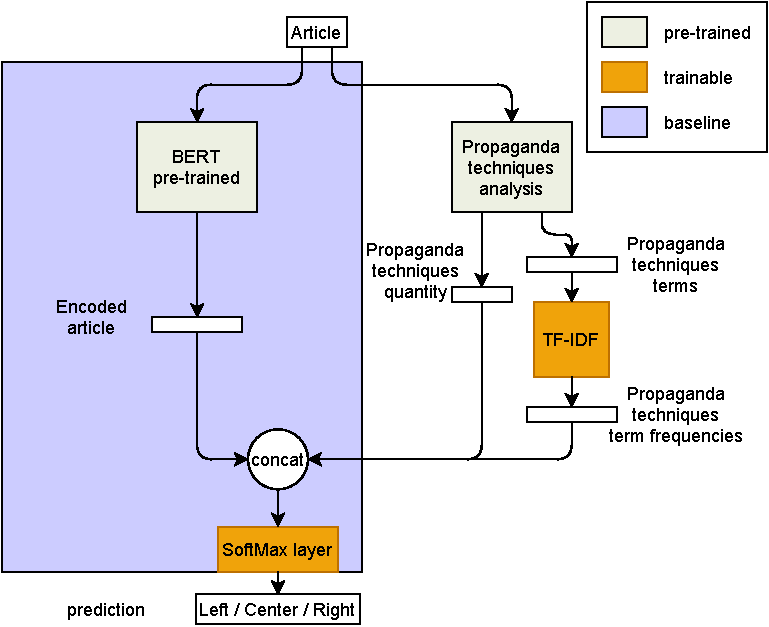
\includegraphics[width=\linewidth]{figures/methodology-Page-1.pdf}
    \caption{The architecture of the model to classify political leaning.}
    \label{fig:model_classifier}
\end{figure}

The setup for the classifier is represented in Figure~\ref{fig:model_classifier}. We can see on the left that we are encoding the articles with a pre-trained BERT model (cf. Section~\ref{ssec:ps_leaning_classifier}). On the right, instead, we are computing the propaganda features and then we inject them into the last layer of our neural network.


\subsubsection{Propaganda Features}


As mentioned earlier, for the propaganda analysis, we use the state of the art approach provided in~\citet{da2019fine}.\footnote{\url{https://huggingface.co/QCRI/PropagandaTechniquesAnalysis-en-BERT}} Their tool extracts 18 propaganda techniques. We apply this tool to the articles in our dataset to obtain these propaganda annotations.
%and we gather the annotation for the articles in the dataset by using the official model released.
%API.\footnote{\url{https://app.swaggerhub.com/apis-docs/yifan2019/Tanbih/}}
%This model provides as result a set of spans from the text with a label corresponding to one of the 18 techniques.
% In addition to the propaganda techniques, we also run lexicon-based sentiment analysers to obtain a set of words loaded with sentiment with their polarity value (positive vs negative).
We use these annotations to calculate several numerical features that we employ in the following three sections to answer the three research questions introduced before.
%\begin{enumerate}
%   \item the total quantity of propaganda (first
%   \item the quantity of each propaganda technique
%   \item the frequency of words that have been annotated for each propaganda technique
%\end{enumerate}

% The extracted features are then fed to a classifier that can be \sout{a SVM or} a Neural Network (single dense layer with softmax activation function).
% The train/test split for the 13k and 60k datasets is done with stratified split (to keep the proportion of L/C/R in the two splits): 90\% train, 10\% test.


% Our analysis workflow %model architecture we use 
% is depicted in Figure~\ref{fig:model_classifier}. 
Each article in the dataset is passed through the baseline BERT pre-trained models to calculate the baseline result, and through our models that incorporate the various propaganda features to calculate the results from our three different subquestions. %\todo{correct?} 
%Each article in the dataset is passed through either the baseline BERT pre-trained models, or the models that incorporate the various propaganda features. 
%The model The orange parts are being trained with the training set: the final SoftMax layer and the term-frequency analysis.

\subsubsection{Metrics}

We calculate the F1-macro and accuracy of the models and compare them with each other and with the baseline. % in search of any changes and improvements.%  we try to understand if there are some improvements for each of the three sections, and what is their statistical significance.
We also evaluate the significance of each added feature from the weight assigned to them %to each features 
by the classification model (the higher the weight, the more discriminative the feature is for Left/Centre/Right-leaning articles). %by looking at the weights of the models used, to understand what they learned.

%In some cases, 
We also combine the features given by each feature set, to see whether the addition of certain features helps to achieve higher classification accuracy. %values for the metrics. 
This combination is performed by concatenating the inputs to the SoftMax dense layer. It is not a combination of trained models, but it is a model that is trained and used on a combination of input features.


\begin{table}[!htbp]
    \centering
    \scriptsize
    %\small
    % \resizebox{\textwidth}{!}{
    \begin{tabular}{l|rr|rr}
                                            & \multicolumn{2}{c}{Random} & \multicolumn{2}{c}{Media}                                                     \\
        Model                               & F1-Macro                   & Accuracy                  & F1-Macro                & Accuracy                \\
        \hline
        \texttt{Majority}                   & 21.0286                    & 46.0769                   & 21.0286                 & 46.0769                 \\
        % \texttt{Baly-API} & 42.3355 & 43.8356 & 42.0523 & 43.6910 & 41.6863 & 41.7993 & & & & \\
        \texttt{Baly-baseline (0)}          & $\star$56.4447             & $\star$58.6153            & 40.8647                 & 46.2307                 \\
        %\texttt{Baly-paper} (*) & 80.19 & 79.83 & 35.53 & 36.75 \\
        \hline
        \texttt{Prop-Total (1)}             & 36.2966                    & 42.3076                   & 28.8285                 & 41.5384                 \\
        \texttt{Prop-Techniques (2)}        & 36.7166                    & 40.6153                   & 33.0682                 & 40.5384                 \\
        \texttt{Prop-Total-Terms (3a)}      & 42.0261                    & 43.5384                   & 41.5915                 & 43.3076                 \\
        \texttt{Prop-Techniques-Terms (3b)} & 42.4357                    & 43.2307                   & 40.8192                 & 41.9230                 \\
        % \texttt{Prop-words-BERT} (3) & 35.4718 & 48.2387 & 35.4718 & 48.2387 \\
        \hline
        \texttt{(0)+(1)}                    & 55.7786                    & 57.7692                   & \textbf{42.1847}        & \textbf{47.5384}        \\
        \texttt{(0)+(2)}                    & 54.9714                    & 56.9999                   & \textbf{42.4362}        & \textbf{$\star$47.6153} \\
        \texttt{(1)+(2)}                    & 36.5217                    & 40.4615                   & 33.6202                 & 41.0000                 \\
        \texttt{(0)+(1)+(2)}                & 55.2121                    & 57.1538                   & \textbf{42.2102}        & \textbf{47.3846}        \\
        \texttt{(0)+(3a)}                   & 54.6287                    & 56.6923                   & \textbf{41.9766}        & \textbf{46.5384}        \\
        \texttt{(0)+(3b)}                   & 54.8004                    & 56.3076                   & \textbf{41.9965}        & 46.2307                 \\
        \texttt{(3a)+(3b)}                  & 44.3506                    & 46.3076                   & \textbf{41.8725}        & 44.3076                 \\
        \texttt{(0)+(3a)+(3b)}              & 53.2549                    & 54.7692                   & \textbf{42.0576}        & 45.92307                \\
        \texttt{(1)+(2)+(3a)}               & 42.0611                    & 43.8461                   & \textbf{42.5401}        & 44.5384                 \\
        \texttt{(0)+(1)+(2)+(3a)}           & 54.0515                    & 56.0769                   & \textbf{42.2358}        & \textbf{46.8461}        \\
        \texttt{(1)+(2)+(3b)}               & 44.3166                    & 45.6153                   & \textbf{41.9613}        & 44.0000                 \\
        \texttt{(0)+(1)+(2)+(3b)}           & 45.6153                    & 45.6153                   & \textbf{41.9292}        & 46.2307                 \\
        \texttt{(1)+(2)+(3a)+(3b)}          & 45.0456                    & 47.2307                   & \textbf{$\star$43.4564} & 45.9230                 \\
        \texttt{(0)+(1)+(2)+(3a)+(3b)}      & 53.6459                    & 53.6459                   & \textbf{42.5509}        & \textbf{46.5384}        \\
    \end{tabular}
    % }
    \caption{Results given by the different features and combinations of features.}
    \label{tab:results_prop_features_classifier}
\end{table}
% \todoHA{Table~\ref{tab:results_prop_features_classifier} p-values?}
% \todomargin{yes ideally, but need to compute for all the values}

Table~\ref{tab:results_prop_features_classifier} shows the results for all the three subsections below, to be able to compare the values all together.
In the first two rows, we can see the values for the two considered baselines (majority voting and BERT-based baseline).
Then, in the second group, we can see the results of the features considered on their own, without combination.
\texttt{Prop-Total} denotes the feature of the total quantity of propaganda, that is used to reply to RQ3.2.1 (Section~\ref{ssec:ps_prop_leaning_classifier_total}).
\texttt{Prop-Techniques} instead indicates the quantities of each propaganda technique, that are used as features to reply to RQ3.2.2 (Section~\ref{ssec:ps_prop_leaning_classifier_techniques}).
\texttt{Prop-Total-Terms} and \texttt{Prop-Techniques-Terms} relate to the term-based features, that are computed with TF-IDF of the propaganda words (first all together, then divided by propaganda technique), and are used to reply to RQ3.2.3 (Section~\ref{ssec:ps_prop_leaning_classifier_terms}).
% Baselines above, RQ3.2.1=\texttt{Prop-Total}, RQ3.2.2=\texttt{Prop-Techniques}, RQ3.2.3= (\texttt{Prop-Total-Terms} and \texttt{Prop-Techniques-Terms}).
Below, in the last group of the table, we can see various combinations of features that in some cases provide improvements over the baseline. \textbf{Bold} means that the score is higher than the baseline. The symbol $\star$ denotes the best result for the column.

\subsection{Total Quantity of Propaganda}
\label{ssec:ps_prop_leaning_classifier_total}


Our hypothesis behind RQ3.2.1 is that the total quantity of propaganda contained in an article helps to recognise its political leaning.
% definition
To answer RQ3.2.1, we
% \todoHA{first?}\todomargin{no, only. more features in other subsections}
consider only the total amount of propaganda detected in each article. For each article, we calculate a single value to represent the percentage of propaganda text inside the article. %Using a percentage compensates for the varying lengths of articles.%These words are the one annotated as propaganda by \citet{da2019fine} (see Section \ref{sec:prop}).
% how it is computed
We use a percentage in order to be less biased and independent of the article size.
This value is computed for each article as the ratio between the number of words detected as propagandist (see previous Section \ref{ssec:ps_prop_leaning_across}) and the total number of words. For example, if an article has 600 words, and propaganda analysis annotated 30 of them as being propagandist, the value of the feature will be 5\%.
% hypothesis
%The hypothesis is that by observing the total quantity of propaganda contained in an article, we can recognise its political leaning.
% stats
As we saw in the previous Section~\ref{ssec:ps_prop_leaning_across} in Figure~\ref{fig:prop_sent_across_leaning}, the distributions of the total quantity of propaganda is quite similar across political leaning, but it has lower values in the Center and higher values in the Right.
%Figure~\ref{fig:tot_quantity} shows how this value is distributed across Left, Centre and Right leaning articles. It appears that all three groups have a similar propaganda distribution. The Centre appears to have slightly less propaganda, and the Right sources have the most (could be due to propaganda bias as we highlight later in Section~\ref{sec:discussion}).%, especially looking at the dots that represent the outliers. 
% TODO better figure
%Overall, the boxplot shows that the presence of propaganda is similar across the board.%, and the results in Table \ref{tab:results_prop_features_classifier} show that adding this feature lowers our classification accuracy. Hence %mostly overlap so this is a negative sign for our hypothesis.
%the answer to RQ3.2.1 is No, the mere presence of propaganda is insufficient to determining the political leaning of articles. 

% TODO: rename categories in plot to L/C/R
% \begin{figure}[!htb]
%     \centering
%     \includegraphics[width=\columnwidth]{figures/total_prop_data_condensed_mod.jpg}
%     \caption{Boxplot of the total amount of propaganda in Left, Centre and Right articles.}
%     \label{fig:tot_quantity}
% \end{figure}

% TODO move baseline considerations to section 3? When model will be shared by baly, this won't exist anymore
% Table~\ref{tab:results_prop_features_classifier} contains in the first group the baselines considered:

% \begin{itemize}
%     \item The \texttt{Majority} baseline, just providing the most common class as output, has quite low results and is considered here just as lower threshold on the other values.
%     \item \texttt{Baly-baseline}, being an emulation of what described in~\citet{baly2020we}, is still far from the 80\% results reported by the authors. For sure the source-code sharing from them that we are waiting will make the results improve
%     % \item \texttt{Baly-API} instead has much lower results that \texttt{Baly-baseline}, and therefore we can conclude that it is definitely not the implementation of the model described in~\citet{baly2020we}. It is coming from the same research group but we need to ask to the maintainers which results is it providing.
% \end{itemize}

\subsubsection{Results}
Table~\ref{tab:results_prop_features_classifier} shows the results of this first feature set under the name \texttt{Prop-Total}. The low values, just above the \texttt{Majority} baseline, indicate that the feature is unsuitable for determining which side an article belongs to. Both F1 and accuracy are below the values of \texttt{Baly-baseline} for both Random and Media splits. Even combining this feature with the baseline (i.e. adding propaganda percentage as features to the BERT model) does not provide an improvement, as shown by the row denoted by \texttt{(0)+(1)}.



% % confusion matrix
% Looking at the confusion matrix of the 60k dataset in Figure~\ref{fig:total_prop_confusion_60k}, we can see that the model learned to predict the class with most articles, with a few exceptions that are classified as Right (probably the articles with a lot of propagandistic content, TODO compare with learned weights). A similar result can be seen in the 13k dataset. If instead we look at the balanced dataset, Figure~\ref{fig:total_prop_confusion_60k_balanced}, the models shifts to predicting random labels between Centre and Right.
% This means that, removing the shortcut~\citep{geirhos2020shortcut} of ``everything belongs to the Left'', the model cannot pick any relevant information from the feature described above.
% For the \texttt{baly} dataset instead,


\begin{figure}[!htbp]
    \centering
    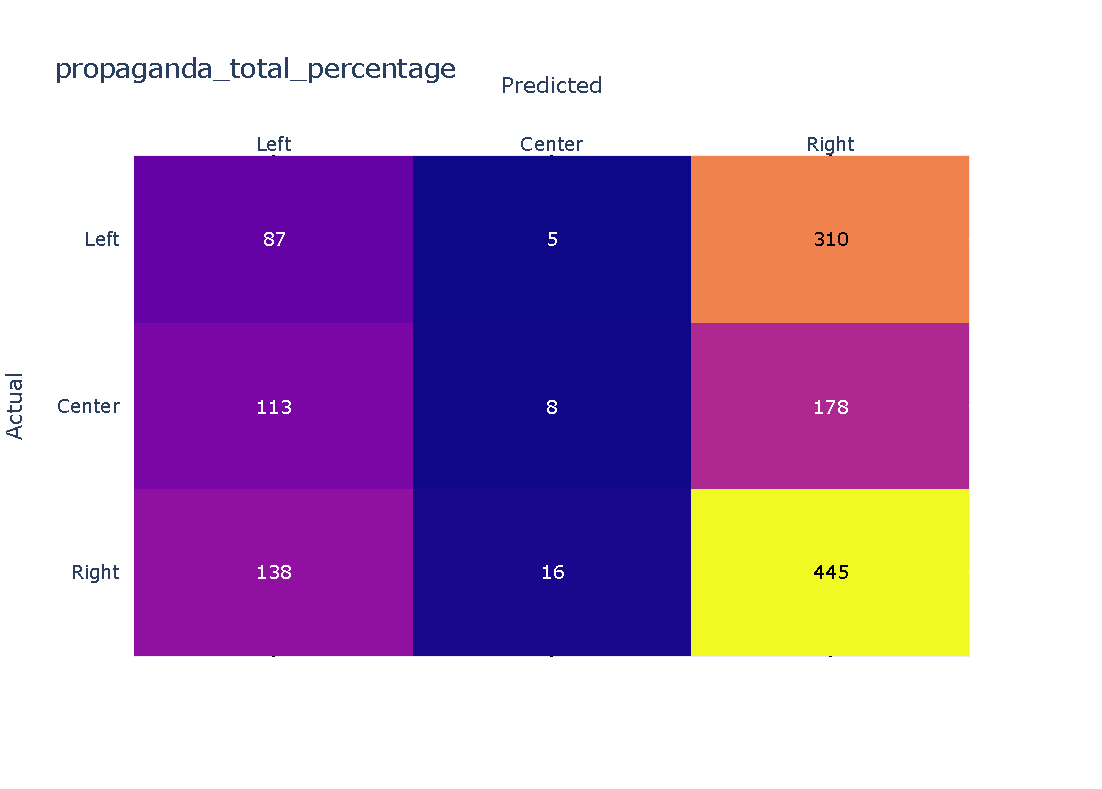
\includegraphics[trim={0.9cm 2cm 0.9cm 1cm},clip,width=0.75\linewidth]{figures/baly_media_confusion_matrix_propaganda_total_percentage.pdf}
    %\vspace{-1cm}
    \caption{Confusion matrix using the \texttt{Prop-Total} features (RQ3.2.1).}
    \label{fig:total_prop_confusion}
\end{figure}

\subsubsection{Confusion Analysis}

The confusion matrix in Figure~\ref{fig:total_prop_confusion} shows that the classifier is introducing biased predictions towards the Right-leaning class. %From observing that in general right-leaning articles contain more propaganda overall (\texttt{Prop-Total} feature), the results are skewed right. 
This results in higher recall but lower precision for the Right class, and almost zero accuracy for the Centre label.

In summary, the answer to RQ3.2.1 is: \textbf{the total amount of propaganda in an article does not seem to be a good indicator of the political leaning of an article}.

% provides a low result overall but a quite good F1 on the Right class.

% \begin{figure}[!h]
%     \centering
%      \begin{subfigure}[b]{0.45\linewidth}
%          \centering
%          \includegraphics[width=\linewidth]{figures/nodes_stratified_confusion_matrix_propaganda_total_percentage.pdf}
%          \caption{imbalanced 60k}
%          \label{fig:total_prop_confusion_60k}
%      \end{subfigure}
%     %  \hfill
%     \begin{subfigure}[b]{0.45\linewidth}
%          \centering
%          \includegraphics[width=\linewidth]{figures/nodes_stratifiedbalanced_confusion_matrix_propaganda_total_percentage.pdf}
%          \caption{Balanced 60k}
%          \label{fig:total_prop_confusion_60k_balanced}
%      \end{subfigure}
%      \\
%      \begin{subfigure}[b]{0.45\linewidth}
%          \centering
%          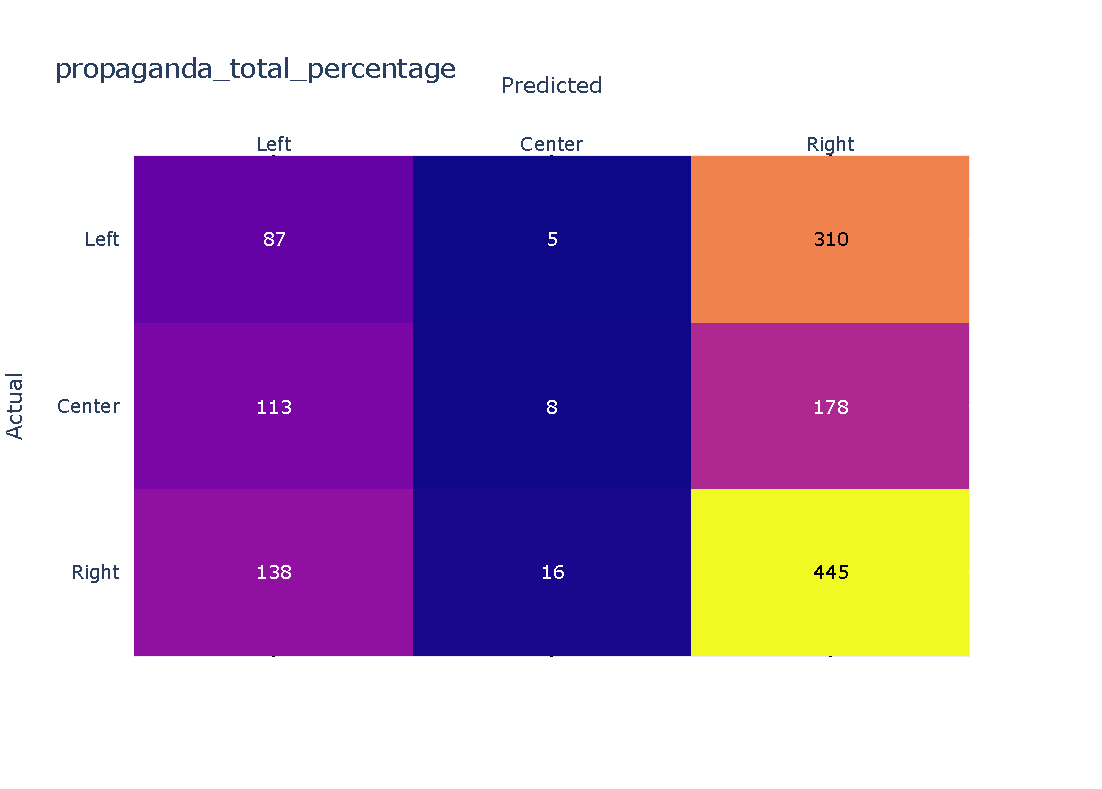
\includegraphics[width=\linewidth]{figures/baly_media_confusion_matrix_propaganda_total_percentage.pdf}
%          \caption{Baly}
%          \label{fig:total_prop_confusion_baly}
%      \end{subfigure}
%     \caption{Confusion matrix of the classifier using the features of \texttt{Prop-Total}.}
%     \label{fig:total_prop_confusion}
% \end{figure}



% TODO: double-check: if we explained the reasons for the classifier, inspecting the weights does not make sense
% % what the model learned:weights
% If we inspect the weights learned by the model in figure~\ref{fig:total_prop_weights}, the network simply learned that propaganda is mostly associated with the Left and not with the Center; the left is in the middle.
% This works well for the left-leaning articles (only 247 out of 2499 are mis-classified) while it does not produce good results for the other two political leanings.
% The decision based only on this feature acts in the following way:
% \begin{itemize}
%     \item if an article has low quantities of propaganda, it is put in the Left bucket (almost all the articles)
%     \item if an article has high quantities of propaganda, it is put in the Right bucket
%     \item no articles are put in the Center bucket (they should have negative quantities, according to the weights)
% \end{itemize}

% \begin{figure}[!h]
%     \centering
%     \includegraphics[width=\linewidth]{figures/total_prop_weights.png}
%     \caption{Weights of the classifier using only the total propaganda quantity: yellow means positive signal and purple means negative signal.}
%     \label{fig:total_prop_weights}
% \end{figure}

% significance

% The last row of Table~\ref{tab:q_60k} presents the combination of this feature with the baseline, which results in a small degradation of the baseline. This feature is not enough to recognise political leaning.


\subsection{Quantity of Particular Propaganda Techniques}
\label{ssec:ps_prop_leaning_classifier_techniques}

In this section, we test the hypothesis of RQ3.2.2, which is that the presence of particular propaganda techniques helps to determine the political-leaning of articles.

%From the negative results to the first research question, we make another step to use more detailed features. 
Instead of relying on a single value representing the total quantity of propaganda, we now consider the amount of each propaganda technique to train the political-leaning classifier.
% The second step we take is to break the quantities of propaganda with respect of each one of the techniques.
The motivation behind is that a specific political leaning (e.g. Right-leaning) may be using one or more techniques more than others, and the classifier could pick these differences to perform its decisions.
This means that our feature vector is not a one-value vector but instead it is an 18-values vector, each one representing the amount of a specific propaganda technique (as also analysed in Section~\ref{ssec:ps_prop_leaning_across}).


We compute the word-based percentage of each technique inside each article. This means that the value for each technique is equal to the number of words belonging to it, divided by the total number of words in the document. A value of 1\% means that 1 out of 100 words in the document have been spotted as being part of the considered propaganda technique.
%We use a percentage, as in the previous case, in order to be independent on the article size.

% TODO: too small and messy figure
% \begin{figure}[!htb]
%     \centering
%     \includegraphics[width=\columnwidth]{figures/baly_prop_techniques_together.pdf}
%     \caption{Distribution of the amount of propaganda techniques in our dataset across Left (blue), Centre (green), and Right (red).}
%     \label{fig:prop_perc}
% \end{figure}

% data distribution
%To give an idea of the computed percentages, we grouped the articles according to their political leaning \textcolor{red}{as determined by AllSides}. 
As we have seen in the previous Section~\ref{ssec:ps_prop_leaning_across},  Figure~\ref{fig:prop_tech_details_across_leaning} was showing that the amount of propaganda techniques detected on this dataset is generally low. The most prominent one is the \texttt{Loaded\_Language} with an average word-based percentage of $1.5\%$.
As in the previous subsection, we observe that articles from the Centre appear to be using less most of the propaganda techniques, %, while Left and Right have higher percentages. This is expected given the overall propaganda use pattern found in the previous experiment.   %However, the difference seems minimal overall. 
but as we noted, there are some techniques which have different shapes (U-shape, triangular shape). Our hope is that an automated classifier is able to pick these different patterns and use them to differentiate the political leaning.


% A similar procedure has been done for the sentiment analysis. First, sentiment words have been extracted by several lexicons (TODO list). In this way every sentiment-loaded term in the articles analysed is associated with its polarity value (positive or negative).
% Then with these annotations we extracted the percentage of positive tokens and negative tokens and used these as input features.


\subsubsection{Results}

% - Classifier with features: results and significance
We train the classifiers as the in previous case and obtain the result indicated by \texttt{Prop-Techniques (2)} in Table~\ref{tab:results_prop_features_classifier}. Although the results show improvement over the previous feature considered, they are still well below the best performing baseline. %This indicates that 
%As for the previous case, we have generally low scores, slightly improved from RQ3.2 on both splits.
The results show that (a) \texttt{Prop-Techniques} alone is insufficient to accurately detect the political leaning of articles (RQ3.2.2), and (b) when \texttt{Prop-Techniques} is added to \texttt{Baly-baseline} (line \texttt{(0)+(2)} in results table), it brings an improvement on the Media split for both the F1 and accuracy measures.


%\begin{enumerate}
%    \item \texttt{Prop-Techniques} alone does not provide good results;
%    \item When \texttt{Prop-Techniques} is added to \texttt{Baly-baseline} in line (0) + (2), it does bring an improvement on the media split for both the F1 and accuracy measures.%, which is even bigger when added to the feature from the previous section.
% \item When \texttt{Prop-Techniques} is added to \texttt{Baly-baseline} on the \texttt{Baly} dataset, it has a big improvement on both F1 and Accuracy
%\end{enumerate}

\subsubsection{Significance Test}

Given the improvements in some cases, we perform an additional test following the approach in~\citet{mcnemar1947note}
to better understand the significance of these results. %if this is just a small effect or if it is something significant.
To perform this test, we build a contingency table by considering two arrays: the first shows when the \texttt{Baly-baseline} produced the correct result on the test set, and the second one shows when the line \texttt{(0)+(2)} (baseline+propaganda techniques quantity) produced the correct result on the Media split. The contingency table, therefore, is the 2x2 matrix as shown in
% Table~\ref{tab:contingency} and 
Table~\ref{tab:contingency2}.

% \begin{table}[]
%     \centering
%     \begin{tabular}{c|c|c}
%         & \multicolumn{2}{c}{(0)+(1)+(2)} \\
%          & incorrect & correct \\
%          \hline
%         (0) incorrect & 2013 & 91 \\
%         (0) correct & 75 & 3868
%     \end{tabular}
%     \caption{Contingency table for 60k}
%     \label{tab:contingency}
% \end{table}

\begin{table}[!htbp]
    \centering
    %    \scriptsize
    \small
    \begin{tabular}{rr|c|c}
                                      &           & \multicolumn{2}{c}{\texttt{(0)+(2)}}           \\
                                      &           & incorrect                            & correct \\
        \hline
        \multirow{2}{*}{\texttt{(0)}} & incorrect & 672                                  & 27      \\
                                      & correct   & 10                                   & 591
    \end{tabular}
    \caption{Contingency table on Media splits.}
    \label{tab:contingency2}
\end{table}


% The first addition, when tested for significance with McNemar test with respect to the baseline, it provided a p-value=0.244 for 60k and p-value=0.608 for 13k. The values means that the contribution is not significant.
% Looking at the values of the contingency table, we can see that for the 60k dataset, adding the features from (1) and (2) made 91 elements of the test set to be correctly classified (misclassified instead from the baseline), but at the same time it brought other 75 elements with a correct label according to the baseline to be incorrectly classified.

% TODO move this in a more visible section, like final discussion? This applies to all the propaganda features
Using the predicted labels of the selected rows on the Media split (last two columns of Table~\ref{tab:results_prop_features_classifier}), the \texttt{(0)+(2)} against baseline resulted in a \textbf{p-value=$0.008$}, which means that the \textbf{improvement is significant}.
Remember that the \textbf{Media split is less biased than the Random split}, since in the Media split the sources of the articles in the test set are not overlapping with the sources of the articles in the training set. If we compare the Random vs Media split results, we can see that while the \texttt{Baly-baseline} drops significantly (more than 15\% F1 and 12\% accuracy), the models based on the features of propaganda have a much smaller drop in these measures (less than 8\% F1 and less than 1\% accuracy).
This means that our models with propaganda features are coping better with articles from ``new sources'' that are unseen in the training set.
The improved generalisation abilities of this feature is perhaps what is driving the significant improvement described above. %can be seen when put in combination with the features of the baseline with the significant improvement described just above \textcolor{red}{(sentence unclear)}. 

\subsubsection{Confusion Analysis}

\begin{figure}[!htbp]
    \centering
    %  \begin{subfigure}[b]{0.45\linewidth}
    %      \centering
    %      \includegraphics[width=\linewidth]{figures/nodes_stratified_confusion_matrix_propaganda_percentages.pdf}
    %      \caption{imbalanced 60k}
    %      \label{fig:prop_tech_confusion_60k}
    %  \end{subfigure}
    % %  \hfill
    % \begin{subfigure}[b]{0.45\linewidth}
    %      \centering 
    %      \includegraphics[width=\linewidth]{figures/nodes_stratifiedbalanced_confusion_matrix_propaganda_percentages.pdf}
    %      \caption{Balanced 60k}
    %      \label{fig:prop_tech_confusion_60k_balanced}
    %  \end{subfigure}
    \begin{subfigure}[b]{0.48\linewidth}
        \centering
        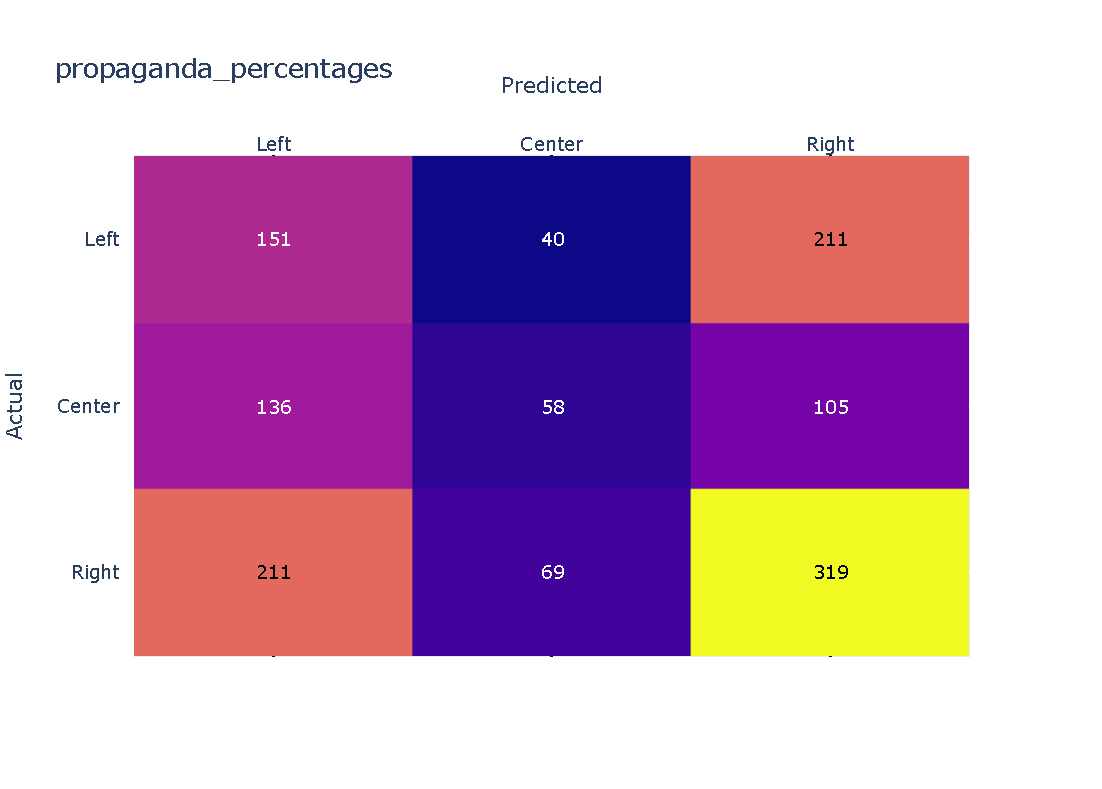
\includegraphics[width=\linewidth]{figures/baly_random_confusion_matrix_propaganda_percentages-small.pdf}
        \caption{Baly random.}
        \label{fig:prop_tech_confusion_baly_random}
    \end{subfigure}
    %  \hfill
    \begin{subfigure}[b]{0.48\linewidth}
        \centering
        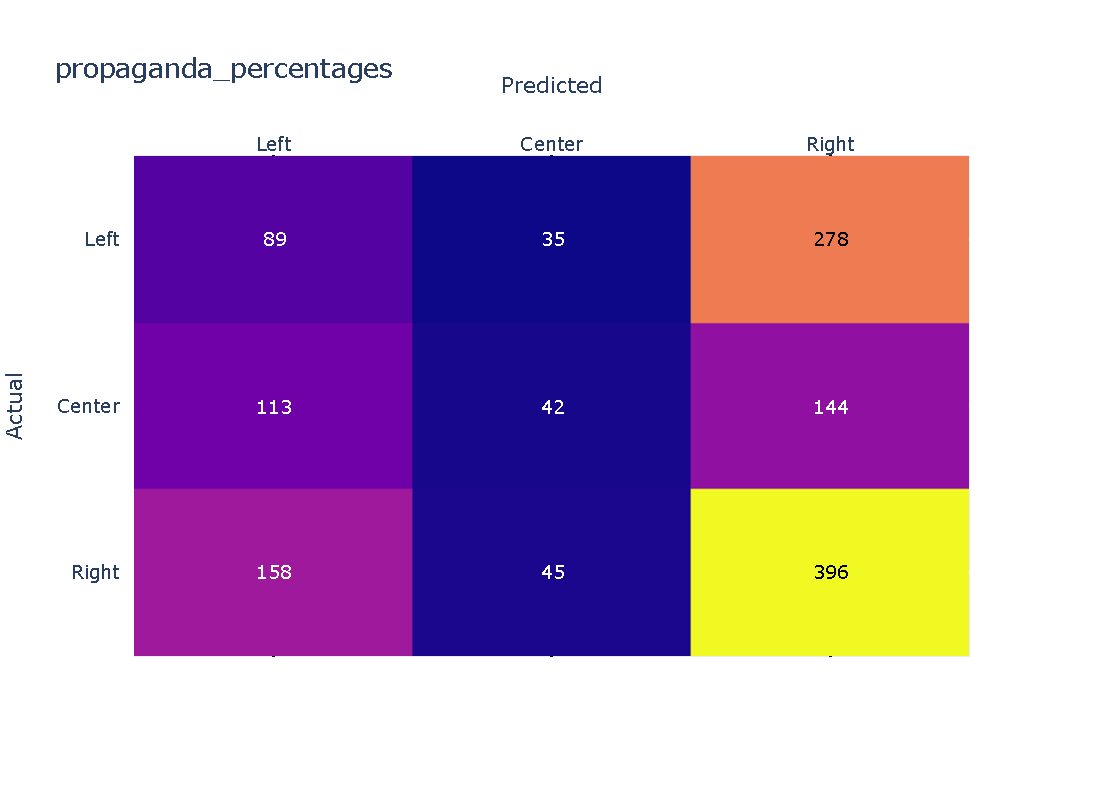
\includegraphics[width=\linewidth]{figures/baly_media_confusion_matrix_propaganda_percentages-small.pdf}
        \caption{Baly media.}
        \label{fig:prop_tech_confusion_baly_media}
    \end{subfigure}
    \caption{Confusion matrix using the features of \texttt{Prop-Techniques} (RQ3.2.2).}
    \label{fig:prop_tech_confusion}
\end{figure}


% confusion matrix
Figure~\ref{fig:prop_tech_confusion} is the confusion matrix for the classifier using the \texttt{Prop-Techniques} feature alone. It shows that the situation is very similar to the previous Subsection~\ref{ssec:ps_prop_leaning_classifier_total}. More articles are predicted as being Right-leaning with respect to the other two classes. %, because it is the most represented class.
% From the imbalanced situation in \ref{fig:prop_tech_confusion_60k}, where the articles were generally predicted to be Left leaning, the subfigure \ref{fig:prop_tech_confusion_60k_balanced} shows that after the correction most of the articles are classified on the Centre.
If we compare the subfigures~\ref{fig:prop_tech_confusion_baly_random} and~\ref{fig:prop_tech_confusion_baly_media}, we see that they are quite similar (F1 and accuracy are very similar too). The only difference is that the Media split predictions are more Right-leaning biased, resulting in lower local F1 for Left and Centre.


\begin{figure}[!htbp]
    \centering
    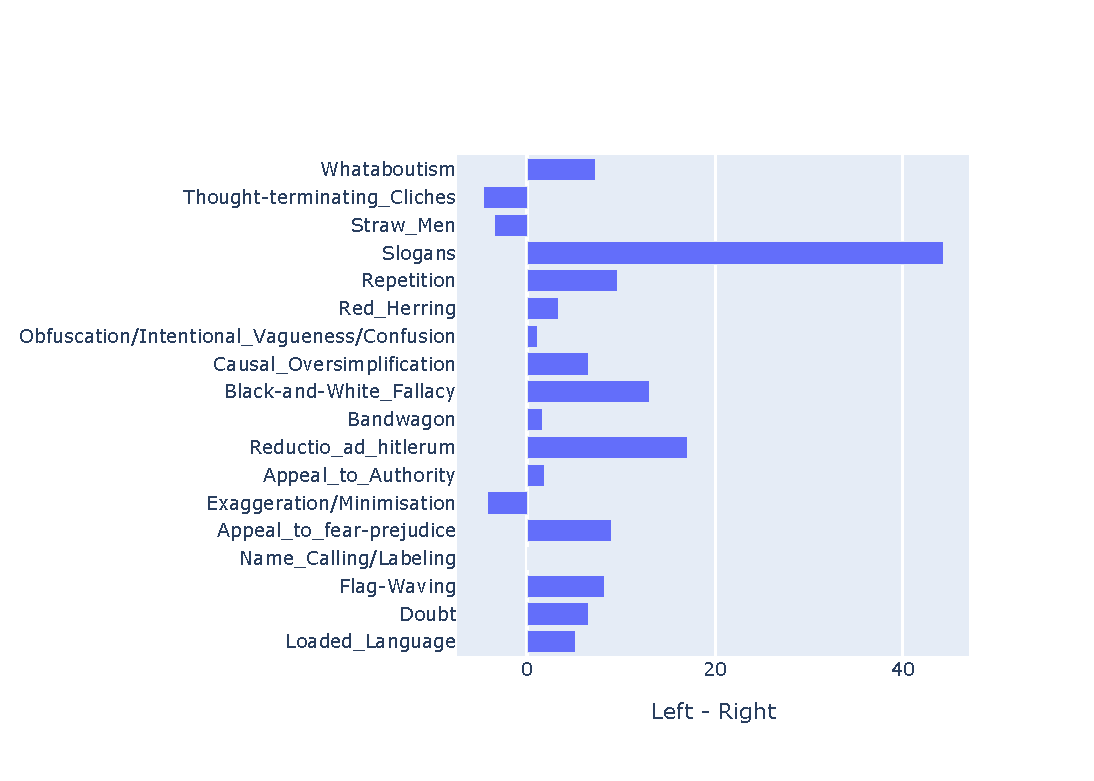
\includegraphics[trim={0cm 0.9cm 2cm 2.5cm},clip,width=\linewidth]{figures/nodes_stratifiedbalanced_weights_propaganda_percentages-small-simple.pdf}
    \caption{Weights for the \texttt{Prop-Techniques} features on the balanced dataset.}
    \label{fig:prop_tech_weights}
\end{figure}

\subsubsection{Feature Importance Analysis}
% features learned
To understand what the model has learnt, we investigate the weights assigned by the neural layer part of the model.
The values are retrieved from the neural network by analysing the weights of the SoftMax layer described before.
For each feature, we have three weights that respectively affect the probabilities assigned to the three output classes (Left, Center, Right).
From these three weights, we compute the difference between the ones for the Right class and the one for the Left class. This computed value represents the association between the specific technique and the output leaning.
We can see in Figure~\ref{fig:prop_tech_weights} the associations learned by the model for the eighteen techniques considered.
Positive values correspond to higher weights for the Right class, while negative values mean that the classifier recognises the appearance of the technique as a sign of being from the Left.

Right is associated with some propaganda techniques (e.g. Slogans and Reductio ad Hitlerum), while the Left is more associated with other techniques (e.g. Exaggeration/Minimisation and Thought-terminating cliches).
% The Centre is generally associated by the model with an absence of all  propaganda techniques.
It is important to note that given the low F1 score of 40\%, the weight assigned by this model for each propaganda technique is only indicative. %does not not represent the ground-truth. 
The model is simply overfitting on the features provided.

%We need to specify that the weights observed do not directly represent the amount of each technique in the corpus. They represent only values that the neural layer assigned as internal weights to optimise the loss on the training set. If the models were having very nice performances we could say that what the model learned is correct, while in this case with values of F1 around 40\% the features learned do not represent quite well the political leaning.



The conclusion for this subquestion RQ3.2.2 is that \textbf{the amount of each propaganda technique is not enough on its own to accurately recognise the political leaning of an article, but when combined with the baseline features produces a significant improvement}.


\subsection{Terms of Propaganda}
\label{ssec:ps_prop_leaning_classifier_terms}

% TODO: keep together propaganda spans instead of tokenizing (e.g., "")
%Given the results of the two previous experiments, and the room for improvement that is left above the scores shown, we want to have a better understanding of the differences between the propaganda coming from multiple political sides.
Following on from the previous two subquestions, we now aim to reach a better understanding of the differences between how propaganda is portrayed in articles belonging to each political side.
We need to go beyond the quantification of detected propaganda techniques (RQ3.2.1 and RQ3.2.2), and investigate the chosen terminology for expressing these propaganda techniques in articles belonging to Left, Right, or Centre (RQ3.2.3). %how the techniques differ across the political spectrum with regards to used language. 
% to recognise political leaning given by the previous sections, the idea is to take a look at the specific terms picked up by the propaganda analysis. Not only quantity, but which words belong to each technique.

%To this end, the RQ3.2.3 considers as features the terms that are picked as part of the propaganda techniques.
The hypothesis is that, even though propaganda techniques are used with similar percentages (as learnt from the first two feature sets), the choice of words and their frequency differ between different-leaning articles, which can improve their classification.
%there are some specific words that are used by opposing leanings that are used with different frequency.
%
In this third part, we proceed with the analysis of terms in two different ways:
\begin{itemize}
    \item (3a) all the propaganda words taken together: non-propaganda annotated words are filtered out. The classifier will then use the remaining propaganda words to learn any differences between political leanings.
          %this acts as an attention mask between the classifier and the articles, filtering out the words that are not propagandist. The classifier will then use the propaganda words to learn any difference between political leanings. 
    \item (3b) propaganda words grouped by propaganda technique: there are 18 groups, one for each propaganda technique. The classifier will use the words, grouped by the technique to which they belong, to recognise the political leaning.
\end{itemize}

While the objective of (3a) is to learn distinctive propaganda terms, (3b) instead focuses on the terms of the 18 individual techniques (e.g. Slogans from the Right might contain different words from the Slogans from the Left).
% \todoHA{You have to add examples whenever and wherever you can}

To obtain the feature vectors of the propaganda words, we use TF-IDF
because its numerical values directly represent single terms. Instead with other embedding methods (e.g., GloVe~\citep{pennington2014glove}, FastText~\citep{joulin2016fasttext}) this correspondence with single terms would be more difficult to extract. By considering the features which get assigned the biggest values in the final SoftMax layer, we can directly say which terms are the most discriminative for the task of political leaning classification.
% since it is easier to link the results to specific terms: the TF-IDF weights that vary the most between political sides are labelled with their feature name (term). 
% the results produced can be easily interpreted. Using State of the Art word embeddings could provide better results but it would be more difficult to understand the importance of specific terms.

\subsubsection{Results}
% results

The row of Table~\ref{tab:results_prop_features_classifier} with the label \texttt{Prop-Total-Terms (3a)} refers to the TF-IDF features computed by only using the propaganda terms, without differentiating between the different techniques.
This row has significantly better results than \texttt{(1)} and \texttt{(2)} on both splits, but only outperform the \texttt{Baly-baseline}  on the Media split in F1. %(not accuracy though). 

On the other hand, the feature \texttt{Prop-Techniques-Terms (3b)} refers to splitting the propaganda terms into the 18 groups and then computing the TF-IDF features on each group separately. The results of this feature set are generally a few decimal points below \texttt{(3a)}.


% % confusion matrix
% To better understand this performance, %where this feature is working and where it is making the prediction fail, 
% we can take a look at Figure~\ref{fig:terms_confusion}, which shows the predictions of the models trained with the features in (3a).
% %TODO: SUBFIGURE DIFFERENCE a/b is NOT RELEVANT. 
% \textcolor{red}{unclear what we learn from this particular confusion matrix. either explain or remove it.  }

% On the imbalanced dataset, the class that has more errors is the Center and the Left side is the most correct, while in the balanced the main diagonal is able to emerge a bit from the other values. On the balanced dataset there is a small bias of the model to say the articles are Right leaning.
% The results and confusion matrix are very similar between the feature (3a) and (3b).

% \begin{figure}[!h]
%     \centering
%      \begin{subfigure}[b]{0.45\linewidth}
%          \centering
%          \includegraphics[width=\linewidth]{figures/nodes_stratified_confusion_matrix_propaganda_tf_idf.pdf}
%          \caption{imbalanced 60k}
%          \label{fig:terms_confusion_60k}
%      \end{subfigure}
%     %  \hfill
%     \begin{subfigure}[b]{0.45\linewidth}
%          \centering 
%          \includegraphics[width=\linewidth]{figures/nodes_stratifiedbalanced_confusion_matrix_propaganda_tf_idf.pdf}
%          \caption{Balanced 60k}
%          \label{fig:terms_confusion_60k_balanced}
%      \end{subfigure}
%     \caption{Confusion matrix of the classifier using the features of \texttt{Prop-Techniques-Terms} (3a).}
%     \label{fig:terms_confusion}
% \end{figure}

% NON-RELEVANT DIFFERENCE BETWEEN A and B 
% \begin{figure}[!htb]
%     \centering
%      \begin{subfigure}[b]{0.48\linewidth}
%          \centering
%          \includegraphics[width=\linewidth]{figures/baly_random_confusion_matrix_propaganda_tf_idf-small.pdf}
%          \caption{Random splits}
%          \label{fig:terms_confusion_random}
%      \end{subfigure}
%     %  \hfill
%     \begin{subfigure}[b]{0.48\linewidth}
%          \centering 
%          \includegraphics[width=\linewidth]{figures/baly_media_confusion_matrix_propaganda_tf_idf-small.pdf}
%          \caption{Media splits}
%          \label{fig:terms_confusion_60k_media}
%      \end{subfigure}
%     \caption{Confusion matrix of the classifier using the features of \texttt{Prop-Techniques-Terms} (3a).}
%     \label{fig:terms_confusion}
% \end{figure}

\subsubsection{Feature Importance Analysis}

% - Classifier with features: features learned?
% BERT: no interpretation?
% TF-IDF weights? TODO
To better understand what the model has learnt, we take a closer look at the neural layer weights assigned to the TF-IDF features.
Figure~\ref{fig:terms_weights_3a} shows the 30 most important terms derived from the weights assigned.
We can see the term ``fit'' emerging as a very representative term of the Centre-propaganda, the terms ``establishment'' and ``suggest'' being significant for the Left, and the terms ``threaten'', ``spread'' and ``prevent'' are mostly associated with the Right-leaning propaganda.


% TODO: make clearer distinction between propaganda label and word
\begin{figure}[!htbp]
    \centering
    \begin{subfigure}[b]{\linewidth}
        \centering
        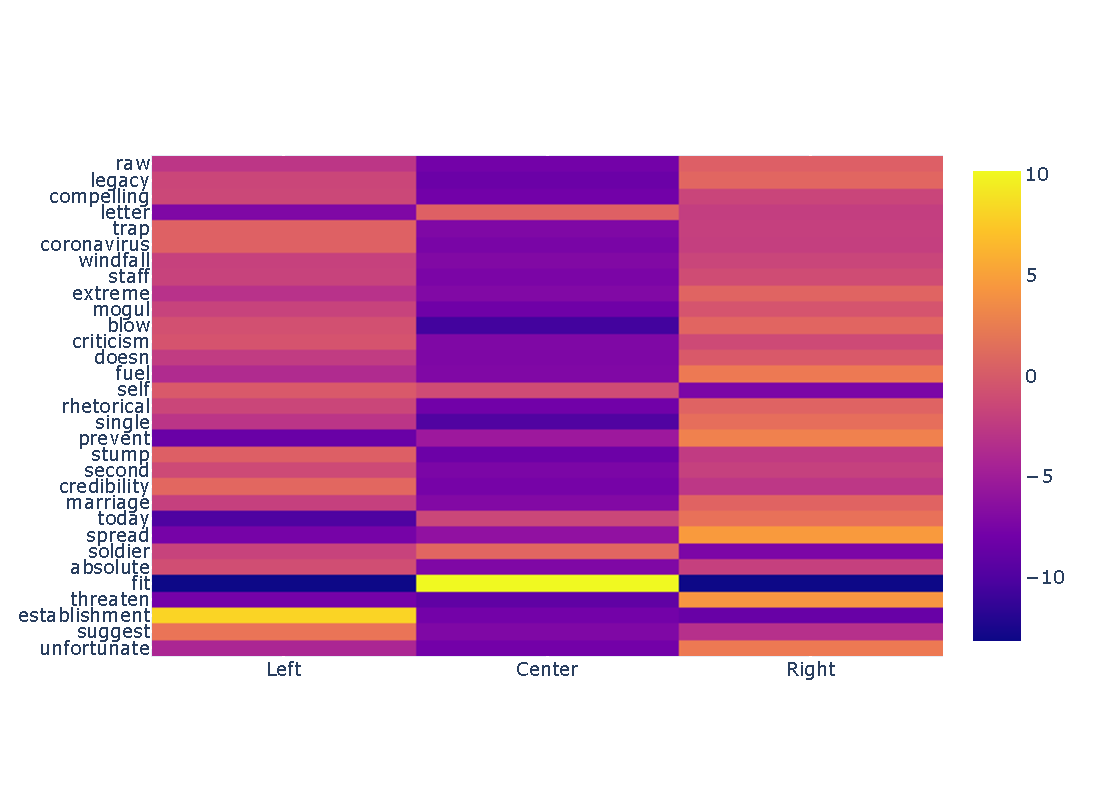
\includegraphics[width=0.75\linewidth]{figures/baly_media_weights_propaganda_tf_idf-small.pdf}
        \caption{\texttt{Prop-Total-Terms}(3a): propaganda terms.}
        \label{fig:terms_weights_3a}
    \end{subfigure}
    %  \hfill
    \begin{subfigure}[b]{\linewidth}
        \centering
        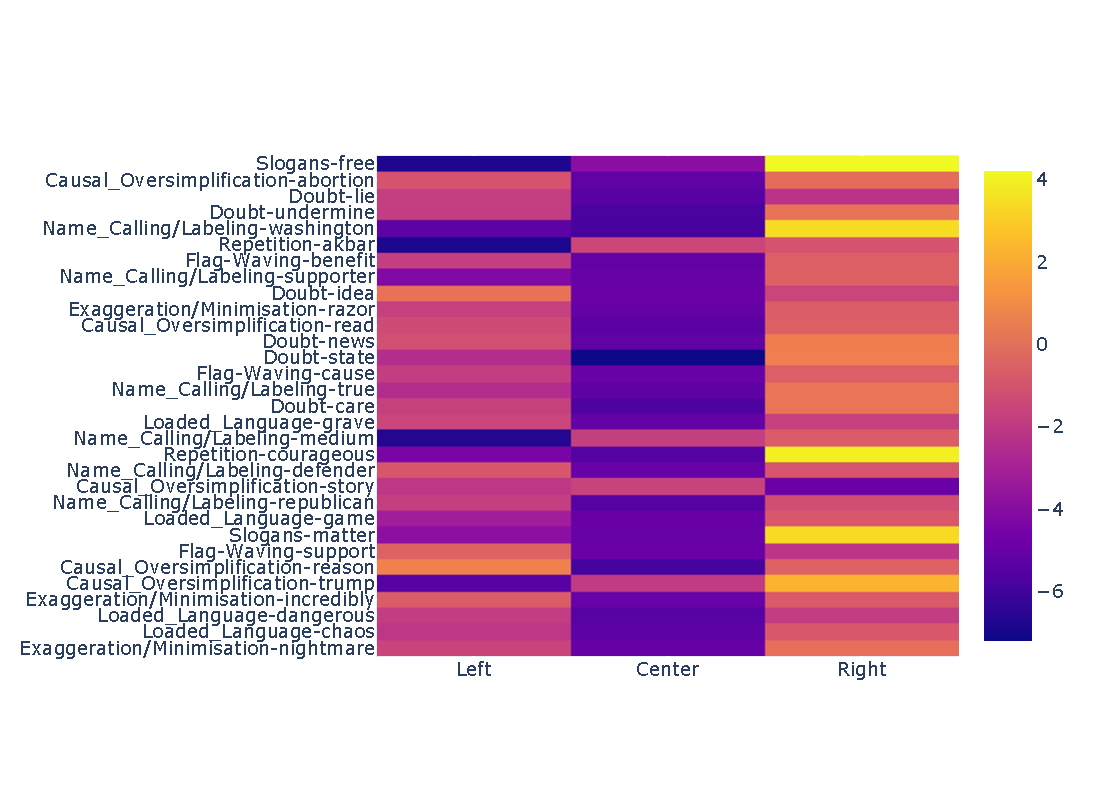
\includegraphics[width=0.75\linewidth]{figures/baly_media_weights_propaganda_techniques_tf_idf-small.pdf}
        \caption{\texttt{Prop-Techniques-Terms} (3b): propaganda terms together with their propaganda technique.}
        \label{fig:terms_weights_3b}
    \end{subfigure}
    \caption{The 30 most important terms learned by the classifier.}
    \label{fig:terms_weights}
\end{figure}
% \todo{barcharts like in \ref{fig:baly_prop_tech_words_all_across_leaning}} --> problem with features and feature names missing / ugly

In Figure~\ref{fig:terms_weights_3b}, we consider each propaganda technique separately. The most discriminating word is ``free'' belonging to the \texttt{Slogans} technique, which has the highest weight for the Right, and the lowest value for the Left. Similar values have the term ``courageous'' (Repetition), ``washington'' (Name Calling) and ``matter'' (Slogans). Terms such as ``idea''(Doubt) and ``support'' (Flag-Waving) instead are mostly associated with the Left-leaning propaganda.

Further investigation is needed to better capture what each of these words means in the context they are used, to determine how to improve on this term analysis.% could be improved and be able to distinguish political sides more effectively.

With the current analysis, we can say that \textbf{the answer to RQ3.2.3 is that the specific propaganda words can only marginally help to classify the political leaning. Using the terms of propaganda we achieve a very similar score to the baseline (rows indicated with \texttt{(3a)} and \texttt{(3b)}), and when added to the baseline features, it helps to achieve a small (but not significant, \textit{p-value=0.657}) improvement}. % NOT SIGNIFICANT IMPROVEMENT: p-value=0.657


\subsection{\statusgreen Reproduction on \texttt{NELA-GT-2018} Dataset}
\label{ssec:ps_prop_leaning_classifier_nela}

% \todo{take from experiment 6 document}
% % 6: classifier (propaganda → leaning) on other datasets

% What: this experiment was reproduced with NELA dataset (MBFC for leaning of the sources)

% Why: The results have similar scores. The significance test is passed but we question whether the results would generalise to other datasets.
% check with other datasets if this behaviour generalises

We have seen in the previous sections that the results of the classifier based on the propaganda features are not setting a big difference in the F1 scores. On the media splits, we managed to increase by a few percentage points (2.59\% F1, 1.38\% accuracy), while on the random splits the baseline still provides the best results.
The feature combination \texttt{(0)+(2)} (baseline and quantity of propaganda techniques), when tested for with McNemar test, resulted significant (p-value $=0.008$).
But we still question whether the results, with such a small margin (F1 and Accuracy) would generalise to other datasets.

For this reason, in this subsection, we take the \texttt{NELA} dataset from Appendix~\ref{app:nela_processing} and we perform the same analysis. In specific, we test on the built subsets denoted with \texttt{NELA-Random-Imbalanced}, \texttt{NELA-Random-Balanced}, \texttt{NELA-Media-Imbalanced} and \texttt{NELA-Media-Balanced}.


The only difference in the experimental setup is that here we are performing a 5-Folds cross-validation instead of a simple train-test.
As discussed in the Appendix, this gives more generalisable results and is less dependent on which articles have been chosen for the test set (particularly when we are using the media splits).

For computing the F1 and accuracy metrics, we accumulate over the 5 folds the values of the true and predicted labels.

\begin{table}[!htbp]
    \centering
    \scriptsize
    %\small
    \resizebox{\textwidth}{!}{
        \begin{tabular}{l|rr|rr|rr|rr}
                                                & \multicolumn{2}{c}{\texttt{Random-Imbalanced}} & \multicolumn{2}{c}{\texttt{Random-Balanced}} & \multicolumn{2}{c}{\texttt{Media-Imbalanced}} & \multicolumn{2}{c}{\texttt{Media-Balanced}}                                                                                                         \\
            Model                               & F1-Macro                                       & Accuracy                                     & F1-Macro                                      & Accuracy                                    & F1-Macro                & Accuracy                & F1-Macro                & Accuracy                \\
            \hline
            \texttt{Majority}                   & 21.5632                                        & 47.8086                                      & 16.6666                                       & 33.3333                                     & 21.5632                 & 47.8086                 & 16.6666                 & 33.3333                 \\
            % \texttt{Baly-API} & 42.3355 & 43.8356 & 42.0523 & 43.6910 & 41.6863 & 41.7993 & & & & \\
            \texttt{Baly-baseline} (0)          & 69.2076                                        & 71.2211                                      & 70.9808                                       & 70.8977                                     & 45.1628                 & 50.5888                 & 46.2165                 & 46.0180                 \\
            %\texttt{Baly-paper} (*) & 80.19 & 79.83 & 35.53 & 36.75 \\
            \hline
            \texttt{Prop-Total (1)}             & 21.5632                                        & 47.8086                                      & 29.5603                                       & 35.2938                                     & 21.7242                 & 47.8372                 & 32.4953                 & 33.0485                 \\
            \texttt{Prop-Techniques (2)}        & 25.6280                                        & 47.8404                                      & 38.4605                                       & 39.7791                                     & 24.2318                 & 46.1973                 & 36.3153                 & 37.5012                 \\
            \texttt{Prop-Total-Terms (3a)}      & 41.3193                                        & 49.6682                                      & 41.8435                                       & 42.3996                                     & 37.0437                 & 45.3760                 & 36.8032                 & 36.8067                 \\
            \texttt{Prop-Techniques-Terms (3b)} & 38.3522                                        & 50.3530                                      & 39.3319                                       & 41.0597                                     & 35.3254                 & 47.3457                 & 35.6495                 & 35.8892                 \\
            % \texttt{Prop-words-BERT} (3) & 35.4718 & 48.2387 & 35.4718 & 48.2387 \\
            \hline
            \texttt{(0)+(1)}                    & \textbf{69.2085}                               & \textbf{71.2271}                             & \textbf{70.9899}                              & \textbf{70.9057}                            & 45.1531                 & \textbf{50.6024}        & \textbf{46.2288}        & \textbf{46.0346}        \\
            \texttt{(0)+(2)}                    & \textbf{69.2905}                               & \textbf{71.2991}                             & \textbf{71.0331}                              & \textbf{70.9510}                            & \textbf{45.1835}        & \textbf{50.6412}        & \textbf{46.3481}        & \textbf{46.1550}        \\
            \texttt{(1)+(2)}                    & 25.7629                                        & 47.8299                                      & 38.5816                                       & 39.8064                                     & 24.4286                 & 46.2459                 & 36.2956                 & 37.1280                 \\
            \texttt{(0)+(1)+(2)}                & \textbf{$\star$69.2994}                        & \textbf{$\star$71.3019}                      & \textbf{$\star$71.0358}                       & \textbf{$\star$70.9529}                     & \textbf{$\star$45.1998} & \textbf{$\star$50.6524} & \textbf{46.3457}        & \textbf{46.1517}        \\
            \texttt{(0)+(3a)}                   & 65.7886                                        & 68.5003                                      & 68.5460                                       & 68.4628                                     & 44.7002                 & 49.4820                 & 46.1694                 & 46.1916                 \\
            \texttt{(0)+(3b)}                   & 66.1823                                        & 68.7194                                      & 68.5074                                       & 68.4349                                     & 45.0300                 & 49.8181                 & \textbf{46.4617}        & \textbf{46.4431}        \\
            \texttt{(3a)+(3b)}                  & 41.4558                                        & 49.5529                                      & 42.5407                                       & 42.6677                                     & 37.0566                 & 45.1370                 & 36.5396                 & 36.5419                 \\
            \texttt{(0)+(3a)+(3b)}              & 65.0796                                        & 67.8463                                      & 67.4347                                       & 67.3705                                     & 44.4791                 & 49.1030                 & 45.9924                 & 46.0147                 \\
            \texttt{(1)+(2)+(3a)}               & 41.6843                                        & 49.9994                                      & 42.2068                                       & 42.7608                                     & 36.9627                 & 45.4902                 & 36.4236                 & 36.4208                 \\
            \texttt{(0)+(1)+(2)+(3a)}           & 65.7779                                        & 68.4993                                      & 68.5715                                       & 68.4921                                     & 44.8164                 & 49.5117                 & \textbf{46.2871}        & \textbf{46.3227}        \\
            \texttt{(1)+(2)+(3b)}               & 38.8414                                        & 50.4508                                      & 39.6869                                       & 41.3132                                     & 35.7261                 & 47.4435                 & 35.8977                 & 36.0895                 \\
            \texttt{(0)+(1)+(2)+(3b)}           & 66.1066                                        & 68.6778                                      & 68.5074                                       & 68.4376                                     & 45.0148                 & 49.8192                 & \textbf{$\star$46.6062} & \textbf{$\star$46.6054} \\
            \texttt{(1)+(2)+(3a)+(3b)}          & 41.7298                                        & 49.8055                                      & 42.6323                                       & 42.7555                                     & 36.8644                 & 45.1150                 & 36.7762                 & 36.8838                 \\
            \texttt{(0)+(1)+(2)+(3a)+(3b)}      & 65.0692                                        & 67.8439                                      & 67.4353                                       & 67.3718                                     & 44.5016                 & 49.1166                 & 46.05313                & 46.0858                 \\
        \end{tabular}
    }
    \caption{Results NELA.}
    \label{tab:results_prop_features_classifier_nela}
\end{table}

Table~\ref{tab:results_prop_features_classifier_nela} shows the results. We denote also in this table with \textbf{bold} the scores that are higher than the baseline, while the $\star$ symbol means indicates the highest score for the column.

\subsubsection{Results}

% Result: similar behaviour
First of all, if we consider the macro categories of baseline / propaganda features / combinations (the main three groups of rows, separated by horizontal lines), we have a similar behaviour with the \texttt{baly} dataset. The propaganda features alone are not enough to go beyond the initial results from the baseline. However, when the features are combined together with the baseline features, we see an increase of the F1-Macro and Accuracy scores.
But in this case, for each of the 4 splitting methods, we have that some feature combinations are better than the baseline.

% random vs media
Comparing Random vs Media splits, we have confirmed also with this dataset that the Media splits are harder to learn. Having the articles from each media source appear only or in the training set or in the testing set, the model finds at prediction time only news articles that come from unknown sources and whose linguistical style is unknown. Therefore, it cannot use the shortcut of simply recognising the news source style and then output the corresponding leaning.

Also here we see that the propaganda features considered on their own have a smaller gap with respect to the baseline in the media splits (less than 10\% in the media splits, almost 30\% in the random splits).
% \todoAW{Be consistent in your precision. Why is this "less than 10\%", but later you have "0.1292 F1"?}
This means that they are able to generalise better with unseen news sources.

These improved generalisation abilities over the media splits, also reflect on the improvements over the baseline:
\begin{itemize}
    \item with \texttt{Random-Balanced}, the delta between \texttt{(0)+(1)+(2)} and \texttt{(0)} is: 0.05\% for both F1 and Accuracy; % , 0.0552\%
    \item with \texttt{Media-Balanced}, the same delta is: 0.12\% F1, 0.13\% Accuracy; % 0.1292 and 0.1337
    \item the best result of \texttt{Media-Balanced} \texttt{(0)+(1)+(2)+(3b)} has greater delta from \texttt{(0)}: 0.38\% F1, 0.58\% Accuracy; % 0.3897 and 0.5874
    \item \texttt{Media-Balanced} has many more rows that are superior to the baseline.
\end{itemize}
% Media the improvement is higher:
% (0.3897\% F1, 0.5874\% accuracy media-balanced (0)(1)(2)(3b))
% (0.1292\% F1, 0.1337\% accuracy media-balanced (0)(1)(2)
% (0.055\% F1, 0.0552\% accuracy random-balanced (0)(1)(2)

The propaganda features, also with this dataset, show better results with the Media splits.

% balanced vs imbalanced
Instead, Balanced and Imbalanced splits have very similar results when considering the Random splits. However, there is some difference in the Media splits, where balancing the dataset leads to more positive results (better than baseline) for the propaganda features.
% But we can see that the gap between the baseline and propaganda features on their own is smaller

Compared to the results over the \texttt{Baly} dataset, we can see that we have far more consistent results (the row of the table that has overall best results is \texttt{(0)+(1)+(2)}, only surpassed in \texttt{Media-Balanced} by better combinations).
This may be the result of the cross-validation process that provides more stable results with respect to a single train-test scenario.

\subsubsection{Significance}
% which results are significant
We then tested for statistical significance all the values that are denoted in \textbf{bold} in Table~\ref{tab:results_prop_features_classifier_nela} with the McNemar test.

\begin{table}[!htbp]
    \centering
    \resizebox{\textwidth}{!}{
        \begin{tabular}{l|r|r|r|r}
            Model                     & \texttt{Random-Imbalanced} & \texttt{Random-Balanced} & \texttt{Media-Imbalanced} & \texttt{Media-Balanced} \\
            \hline
            \texttt{(0)+(1)}          & .741                       & .717                     & .457                      & .408                    \\
            \texttt{(0)+(2)}          & \textbf{.003}              & .088                     & .055                      & \textbf{1.15e-5}        \\
            \texttt{(0)+(1)+(2)}      & \textbf{.001}              & .069                     & \textbf{.015}             & \textbf{1.68e-5}        \\
            \texttt{(0)+(3b)}         &                            &                          &                           & \textbf{1.45e-5}        \\
            \texttt{(0)+(1)+(2)+(3a)} &                            &                          &                           & \textbf{.004}           \\
            \texttt{(0)+(1)+(2)+(3b)} &                            &                          &                           & \textbf{2.77e-9}
        \end{tabular}
    }
    \caption{p-values of features set that have improvements in NELA dataset.}
    \label{tab:pvalues_nela_classifier}
\end{table}

The results are shown in Table~\ref{tab:pvalues_nela_classifier}, that is showing the p-values. We indicate in \textbf{bold} the values that satisfy the threshold of significance (0.05) and are therefore significant. Some cells are not shown because the corresponding F1/Accuracy values are lower than the baseline.

We can see that only some of the results pass the significance test. The \texttt{Media-Balanced} passes it for almost all the feature sets, with very low p-values.

% \texttt{(0)+(1)}
% - random imbalanced: statistic=1166.000, p-value=0.741 --> non-significant
% - random balanced: statistic=455.000, p-value=0.717 --> non-significant
% - media imbalanced: statistic=1286.000, p-value=0.457 --> non-significant
% - media balanced: statistic=409.000, p-value=0.408 --> non-significant

% \texttt{(0)+(2)}
% - random imbalanced: statistic=2636.000, p-value=0.003 --> significant
% - random balanced: statistic=1035.000, p-value=0.088 --> non-significant
% - media imbalanced: statistic=2942.000, p-value=0.055 --> non-significant
% - media balanced: statistic=991.000, p-value=0.0000115649 --> significant


% \texttt{(0)+(1)+(2)}
% - Random imbalanced: 
% contingency: [[ 79823.   2552.]
%              [  2321. 201539.]]
% statistic=2321.000, p-value=0.001 --> significant

% - Random balanced:
% Contingency: [[ 42684.   1061.]
%              [   978. 105592.]]
% statistic=978.000, p-value=0.069 --> non-significant

% - Media imbalanced:
% [[138562.   2870.]
%  [  2688. 142115.]]
%  statistic=2688.000, p-value=0.015 --> significant

% - Media balanced:
% [[79961.  1182.]
%  [  981. 68191.]]
% statistic=981.000, p-value=0.0000168321 --> significant

% \texttt{(0)+(3b)}:
% - media balanced:
% [[69993. 11150.]
%  [10511. 58661.]]
% statistic=10511.000, p-value=0.0000145614 --> significant

% \texttt{(0)+(1)+(2)+(3a)}:
% [[67978. 13165.]
%  [12707. 56465.]]
%  statistic=12707.000, p-value=0.0044935554 --> significant

% \texttt{(0)+(1)+(2)+(3b)}:
% [[69691. 11452.]
%  [10569. 58603.]]
% statistic=10569.000, p-value=0.00000000277 --> significant

But also with this dataset, even if the results are statistically significant, the margins are very narrow.
As noted before, the highest delta of improvement in Table~\ref{tab:results_prop_features_classifier_nela} is 0.38\% F1 and 0.58\% Accuracy.

\subsubsection{Confusion Analysis}

We want to understand with this dataset what the models learn. Here we analyse the confusion matrices and in the next paragraph the feature importances.


% random unbalanced:
% - tot quantity, prop tech quantities: predict almost everything Right
% - bert vs bert+1+2 (significant): 
%   - actual Left (correct almost the same, wrong from Right to Center)
%   - actual center (more correct, from L and R to center)
%   - actual Right (more correct, from L to C, from C to R)

% random balanced:
% - tot quantity: predict almost everything center/right
% - prop tech quantities: mostly center/right
% - bert vs bert+1+2 (not significant):
%   - actual Left (+20 correct, 10 from Center 10 from Right)
%   - actual Center (from Center to L and R --> wrong)
%   - actual Right (86 from L to R --> good)

% media unbalanced:
% - tot quantity: all Right
% - prop tech quantities: almost all Right (some Left)
% - bert vs bert+1+2 (significant):
%   - actual Left (+66 correct, 100 from Right to Center)
%   - actual Center (-9 correct, 30 from Left to Right)
%   - actual Right (+125 correct, center +60 from Left)

% media balanced:
% - tot quantity / tech quantities: way more balanced, but still bias towards 
% - bert vs bert+1+2 (significant):
%   - actual Left (+61 correct, 46 more in Center, 107 less Right --> good)
%   - actual Center (+161 correct, -137 Left, -24 Right --> good)
%   - actual Right (-21 Right, +49 Center, -28 Left)
% - bert vs bert+1+2+3b (significant, best)
%   - actual Left (-1359 correct, -396 Center, +1755 Right --> very bad)
%   - actual Center (+689 correct, -2286 Left, +1597 Right --> bad)
%   - actual Right (+1553 correct, +781 Center, -2334 Left --> very good)

% Figures to include: 2 columns (splits), 3 rows (models)
% random unbalanced:
% - bert: good for R and also (less for L), not good for center
% - prop quantities: Right bias
% - combined:

% media balanced:
% - bert left bias in prediction
% - prop quantities Right/Center bias
% - combined: drifting a bit to the Right (and problems? what is better? still unbalanced to Left)

\begin{figure}[!htbp]
    \centering
    \begin{subfigure}[b]{0.7\linewidth}
        \centering
        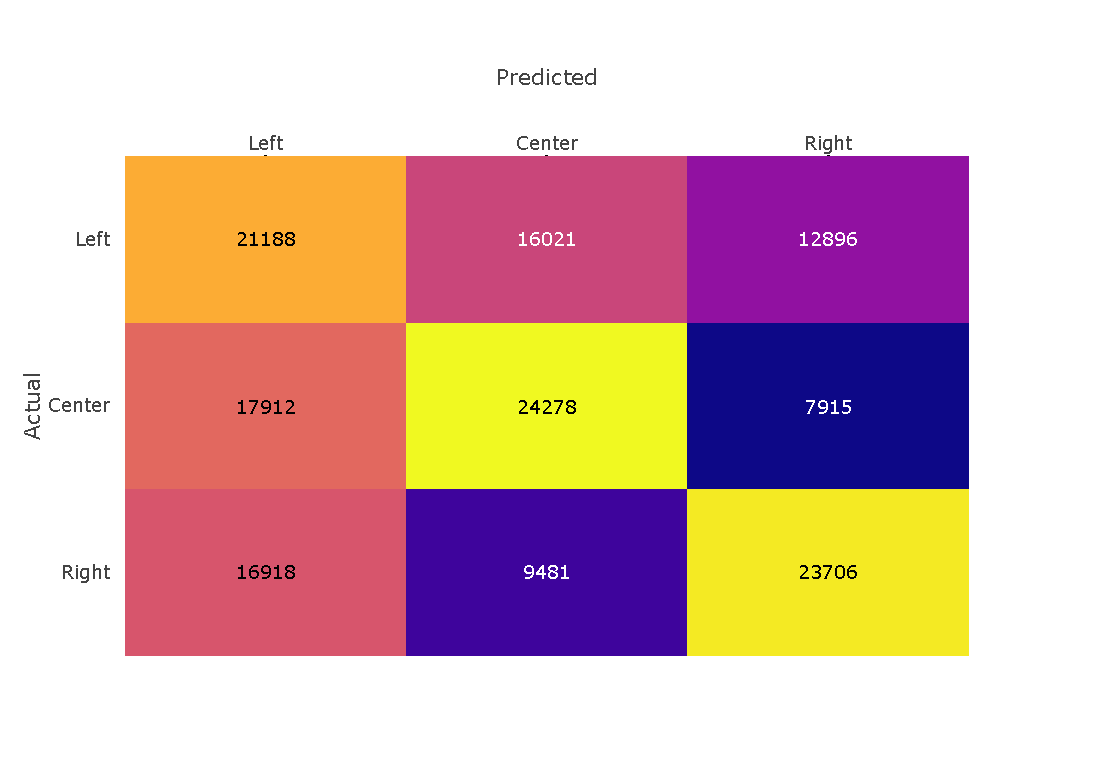
\includegraphics[trim={0 2cm 2cm 1cm},clip,width=\linewidth]{figures/nela_allsides_subset_media_balanced_confusion_matrix_bert.pdf}
        \caption{Baseline: \texttt{Baly-baseline (0)}.}
        \label{fig:nela_confusion_bert}
    \end{subfigure}
    %  \hfill
    % \begin{subfigure}[b]{0.48\linewidth}
    %      \centering 
    %      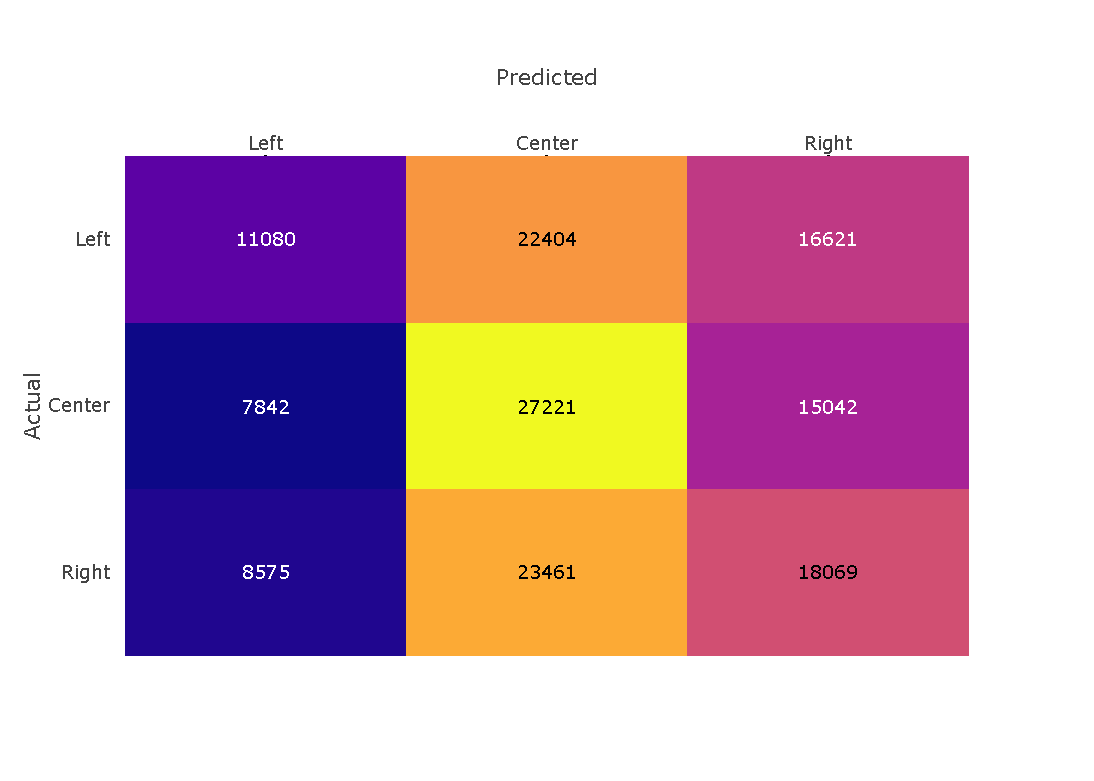
\includegraphics[trim={0 2cm 2cm 1cm},clip,width=\linewidth]{figures/nela_allsides_subset_media_balanced_confusion_matrix_propaganda_percentages.pdf}
    %      \caption{\texttt{Prop-Techniques (2)}}
    %      \label{fig:nela_confusion_prop_quantities}
    %  \end{subfigure}
    \begin{subfigure}[b]{0.7\linewidth}
        \centering
        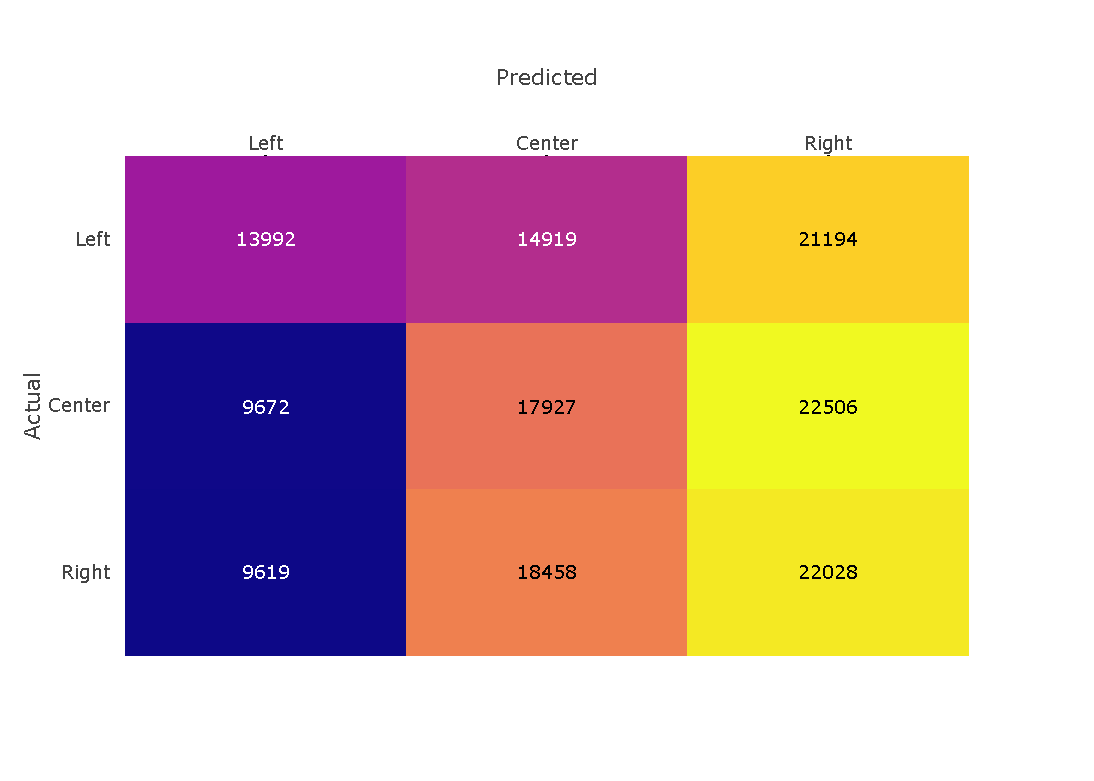
\includegraphics[trim={0 2cm 2cm 1cm},clip,width=\linewidth]{figures/nela_allsides_subset_media_balanced_confusion_matrix_propaganda_techniques_tf_idf.pdf}
        \caption{\texttt{Prop-Techniques-Terms (3b)}.}
        \label{fig:nela_confusion_prop}
    \end{subfigure}
    \begin{subfigure}[b]{0.7\linewidth}
        \centering
        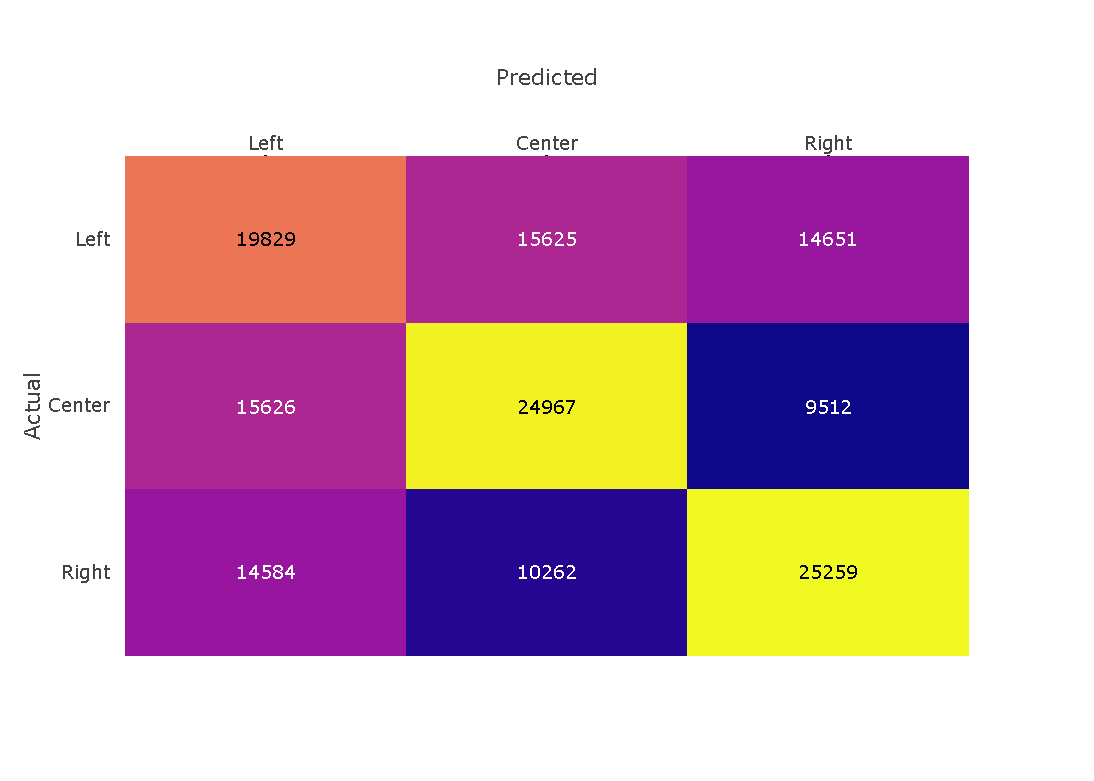
\includegraphics[trim={0 2cm 2cm 1cm},clip,width=\linewidth]{figures/nela_allsides_subset_media_balanced_confusion_matrix_bert,propaganda_total_percentage,propaganda_percentages,propaganda_techniques_tf_idf.pdf}
        \caption{Combination: \texttt{(0)+(1)+(2)+(3b)}.}
        \label{fig:nela_confusion_combined}
    \end{subfigure}
    \caption{Confusion matrix with different features on NELA dataset.}
    \label{fig:nela_confusion}
\end{figure}

Figure~\ref{fig:nela_confusion} shows the inspection of the confusion matrix from three feature sets on the \texttt{Media-Balanced} splits.
In Subfigure~\ref{fig:nela_confusion_bert} we can see that the baseline is having problems with the Left.
On one side, articles that are actually from the Left are being predicted as being from the Center and Right.
At the same time, articles from Center and Right are being predicted as being from the Left. This results in the model being biased towards the Left (56018 articles, with respect to the actual 50105).

In Subfigure~\ref{fig:nela_confusion_prop} instead, we see that the considered propaganda feature has a strong bias towards the Right, as it predicts mostly Right and Center classes (65728 articles, compared to the actual 50105).

By combining the baseline feature with many propaganda features (\texttt{(0)+(1)+(2)+(3b)}) that all have this bias towards the Right, the previous Table~\ref{tab:results_prop_features_classifier_nela} showed that we have an improvement and this improvement tested as significant.
Subfigure~\ref{fig:nela_confusion_combined} shows what happens in details. The overall bias of the BERT baseline is compensated with the bias of the propaganda features (predictions: 50039 Left, 50854 Center, 49422 Right).
The values on the main diagonal are higher for the Right (+1553) and the Center (+689), while they are lower for the Left (-1359).

In the other splits we have a similar behaviour when comparing \texttt{(0)+(1)+(2)} to the baseline. We selected this example because it has the highest delta in F1 and Accuracy, and highest significance.

% media balanced:
% - bert left bias in prediction
% - prop quantities Right/Center bias
% - combined: drifting a bit to the Right (and problems? what is better? still unbalanced to Left)
% - bert vs bert+1+2+3b (significant, best)
%   - actual Left (-1359 correct, -396 Center, +1755 Right --> very bad)
%   - actual Center (+689 correct, -2286 Left, +1597 Right --> bad)
%   - actual Right (+1553 correct, +781 Center, -2334 Left --> very good)

\subsubsection{Feature Importance Analysis}

For the feature importance, we have very similar weights in the \texttt{Prop-Total} and \texttt{Prop-Techniques} with respect to the \texttt{Baly} dataset.

For the propaganda terms, we analyse here the weights given to the \texttt{Prop-Techniques-Terms (3b)} on the \texttt{Media-Balanced}, that is the feature that we analysed above for the confusion analysis.

\begin{figure}[!htbp]
    \centering
    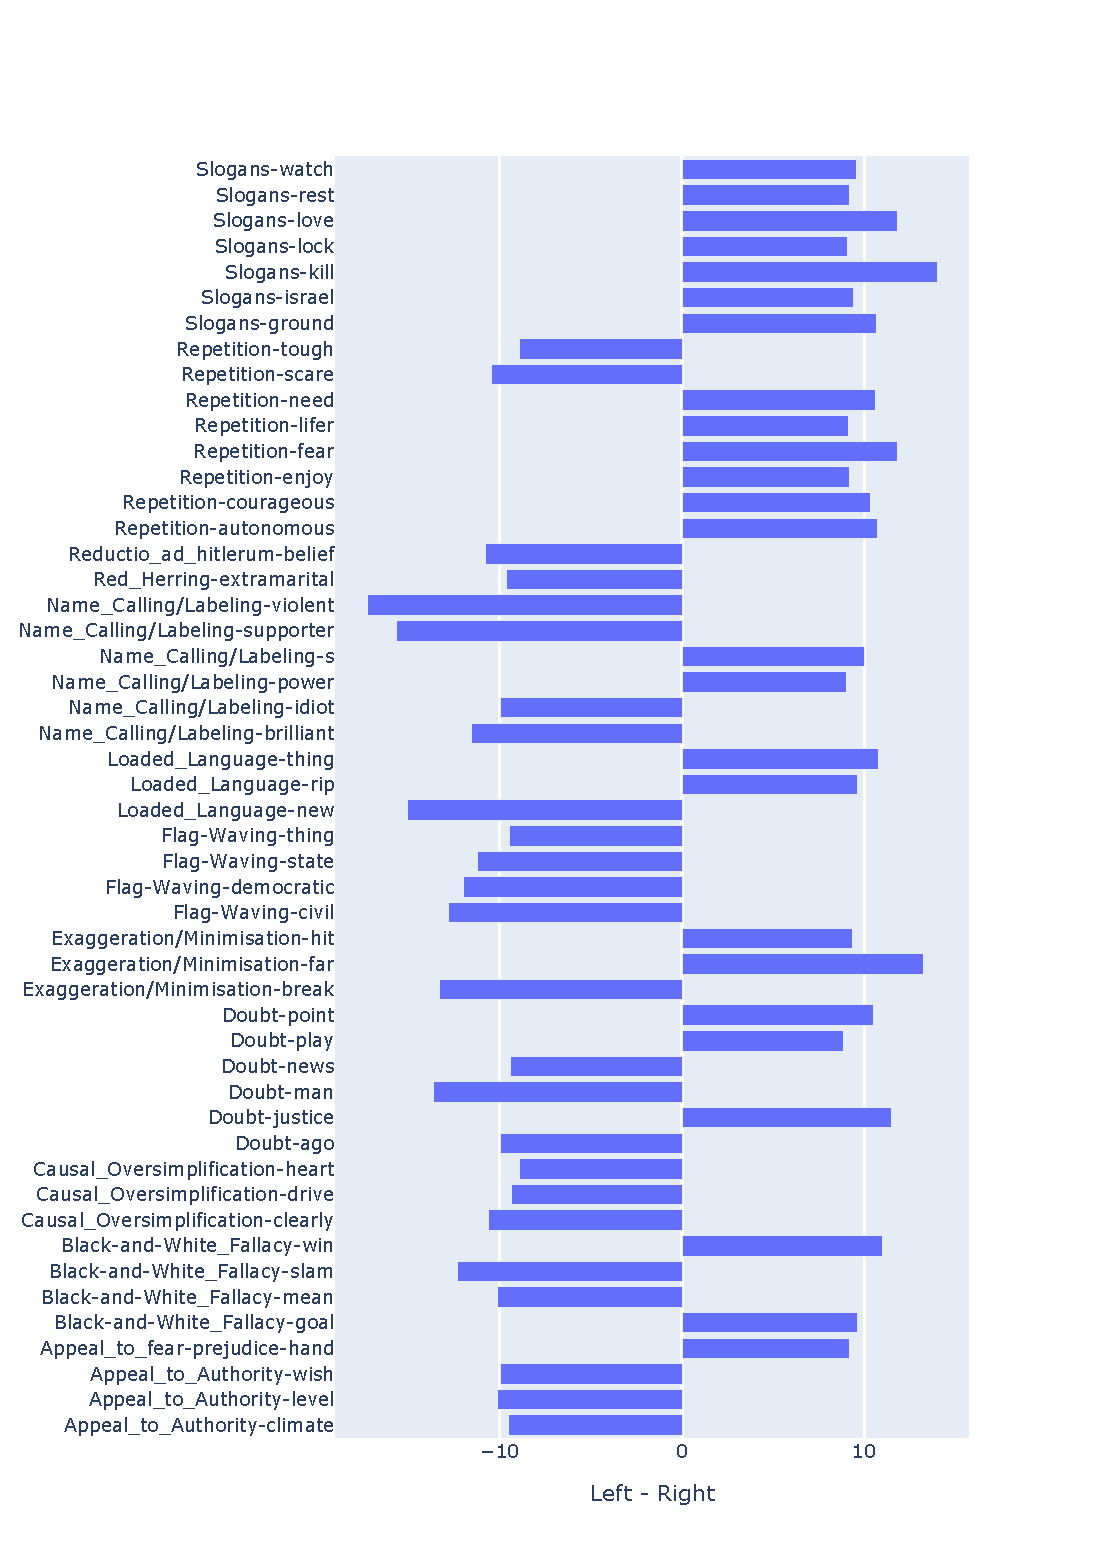
\includegraphics[trim={0 1cm 0 1cm},clip,width=\textwidth]{figures/nela_allsides_subset_media_balanced_weights_propaganda_techniques_tf_idf_2-simple.pdf}
    \caption{Feature weights of \texttt{Prop-Techniques-Terms (3b)} on NELA dataset.}
    \label{fig:nela_weights_prop_tech_terms}
\end{figure}
% \todo{barchart like in \ref{fig:baly_prop_tech_words_all_across_leaning}}

We can see in Figure~\ref{fig:nela_weights_prop_tech_terms} that we have most of the terms more associated with the Left and Right, and less with Center. We can note that the term \textit{power} in the \texttt{Name\_Calling} technique is associated by the model to the Right. Or also \textit{justice} in \texttt{Doubt}, or \textit{kill} in \texttt{Slogan}.
In the Left instead we can notice \textit{violent} in \texttt{Name\_Calling}, \textit{civil}, \textit{democratic} and \textit{state} in \texttt{Flag\_Waving}.



\subsection{Discussion}
\label{ssec:ps_prop_leaning_classifier_discussion}

\begin{comment}
% Issues:

% DRAFT 1
% - data AllSides
%     - the leaning still at the author level, single articles may be from a different leaning. baly paper solution to learn the author instead of the media outlet is a step forward, but still does not represent the leaning of single articles (weak supervision). what could be done to improve it? observe alignment of viewpoint of article towards sensitive topics (pro/against): aspect-based --> my direction
% - data propaganda:
%     - propaganda corpus is only made from extreme right-leaning articles. Solution? Collect also left-leaning propaganda articles (out of scope)
%     - the propaganda annotation tool (now finally available) results in probably being biased to recognise right-leaning propaganda.
% - complexity of the task (recognising political leaning):
%     - same words used with different meaning (cit. seargeant). The context may help
%     - same techniques may be used with the same terms by opposing leanings
%     - terms/propaganda


% DRAFT 2
% Political leaning:
% - AllSides annotates at the author level (more granular than only the News Outlet level but is still distant supervision)
% - How good is the AllSides annotation? Compared to other political leanings of sources? (Media Bias/Fact Check or AdFontesMedia or Wikipedia)
% - The practical definition of political leaning: stance towards a set of topics/issues. An article from an Leftist author may contain right-leaning arguments
% POSSIBLE SOLUTION: 
% Propaganda:
% - Only extreme-right sources in the dataset of propaganda (data problem reflecting on the tool of propaganda detection)
% Intrinsic complexity of the task
% - Same words with different meaning
% - Same propaganda techniques used with same words
% - Reported speech is (should) be the same (does not depend on the news, but on the politician involved), exception of selection bias on what to be reported
\end{comment}

%%%%%% The below is to explain why not use the source. 
%Automated detection of political-leaning is still in its infancy. Although the political-leaning of articles could sometimes be gauged by their sources, there are many examples where articles' political leaning differ from that of their sources, or the sources' leanings are not well known, or the sources themselves are unknown. Hence there is a need for such detection to be based on the text of the article, rather than on where the article came from. 

In this section, we highlight various issues and directions that we found while experimenting with the classifier.
%present the issues that we discovered with this research. The first group relates to the political leaning, while the second one to propaganda.

\begin{comment}
% political leaning issues
%In the problems related to political leaning, we have issues that come from the data used.

%AllSides annotates at the author level. This is more granular than only the News Outlet level provided by other openly-available evaluations (such as Media Bias/Fact Check and AdFontesMedia), but it is still distant supervision.

% It also comes natural to ask how good is the AllSides annotation? Compared to other political leanings of sources, such as Media Bias/Fact Check or AdFontesMedia or Wikipedia, we can do a comparison of the leanings assigned to the sources. TODO this comparison.

This main limitation, of still annotating the leaning of the writer instead of evaluating singularly the leaning of the single articles, is probably something that needs to be analysed a bit closer.
\emph{At this point, we need to reconsider the definition of political leaning as the stance towards a set of topics/issues}. This is supported by the types of questions that are contained in surveys aimed at computing one's personal political leaning\footnote{\url{https://www.allsides.com/rate-your-bias}}. An article from a leftist author may contain right-leaning arguments.
In this work, with the third research question, we are aiming to find the terms more related to left, centre and right propaganda. Still, this analysis needs to be contextualised to be able to distinguish the same term appearing in both left and right propaganda.
% We may find discrepancies between the labels given to an article and singular pieces of text contained.
% The ground truth information could be extracted by ``AllSides Common perspectives'' \url{https://www.allsides.com/rate-your-bias} or \url{https://en.wikipedia.org/wiki/Left-wing_politics} and ``General Positions'' in  \url{https://en.wikipedia.org/wiki/Right-wing_politics}.
% Or it could also be extracted from the articles in the training set, learning the stance towards the entities like in ~\citet{chen2017opinion}.
\\

On the side of automated propaganda analysis, we need to clarify that we are using an experimental tool that therefore has many limitations.
% propaganda issues
Current work in automated propaganda analysis does not take into consideration political leaning, and seems to be focusing on Right-leaning propaganda mostly.
% Right-leaning propaganda is easier to spot because it is usually stronger and it is easier to see from the Left-perspective as opposed. There may be a bit of left-leaning in academia that facilitates this.
The results of this bias can be seen in the dataset collected by~\citet{baly2020we} (as noted in Section~\ref{ssec:related_prop}, the training of the propaganda tool is performed against right-leaning sources) and reflects on the annotations that are provided by the tool we are using.

We acknowledge the intrinsic complexity of distinguishing left and right propaganda usage (dictated by the limitations listed above), especially if we consider that the differences we are talking about may be very subtle and challenging to pick.
For example, the same words can be used with different meaning/targets (e.g. ``enemies of the people'', ``people's will'', ...)~\citep{seargeant2020art}. This results in the same propaganda techniques used with the same words.
% % reported speech problem
% When inspecting the annotations of propaganda, we can see that a representative proportion of propaganda belongs to reported speech from public figures. In this case propaganda is not used by the reporter so we should have a method that accounts for this difference. Reported speech is (should be) the same (does not depend on the news, but on the politician involved), exception of selection bias on what to be reported.



% together issues


% The results do not bring big improvements to the State of the Art in political leaning prediction. The issues found are:

% \begin{itemize}
%     \item The effect of the features considered do not bring big improvements according to F1 and accuracy metrics. In some cases it is possible to achieve small improvements, and some of them are statistically significant. However, we want to improve the analysis and get even better results in all the cases.
%     \item Some of the models trained are probably overfitting on some small differences in the training set. Doing a comparison between the features learned and the actual distribution of the features in the dataset, we can clearly see that small differences in quantities have been amplified by the models, and this results in poor performances even on the training sets (with training accuracy observed not above 65\%)
% \end{itemize}

\end{comment}



% Limitations
\subsubsection{Imbalance in Propaganda Detection}
One limitation is that only articles from the Right political spectrum were used for training the propaganda detection tool provided in \citet{da2019fine}. %, which we use in our analysis. 
As we saw in our first experiment, propaganda is not limited to any particular political leaning. Therefore, propaganda annotations and model training should be less biased to a particular political leaning, and propaganda from all political directions should be used to train such models in the future, which is likely to enhance our results given our balanced dataset. We analyse this limitation in the next experiment in Section~\ref{ssec:ps_prop_leaning_imbalanced}.

\subsubsection{Baseline Incomparability} %with the real baseline of~\citet{baly2020we}.
As noted in Section~\ref{ssec:ps_leaning_data}, the shared dataset by \citet{baly2020we} differs from the one described in their paper, producing incompatibility issues between our results and theirs. %the ones they report.
Additionally, re-implementing their model could have introduced other minor differences. Therefore, we believe that comparing the results from our models with those we obtained from re-implementing the model of \citet{baly2020we} offers a fairer approach. %We will repeat our tests if their model becomes available, and will continue to seek other compatible baselines once other article-specific political leaning detection models become available. 

Also related to comparabilty, we have to underline that the splits shared with the \texttt{baly} dataset (especially the media splits) may not be the best strategy, as we have seen across the cross-validation performed on the media splits of the \texttt{Nela} dataset, results change quite significantly across the folds because very different news sources are used for training/testing. Therefore, using cross-validation provides results that are way more meaningful and representative of the whole dataset.

\subsubsection{Meaning and Context}
As shown in experiment 3, some terminologies are common to Left, Right, and Centre articles. In political narrative, many words tend to be used frequently by different political-leaning groups, but for different meanings or to refer to different groups \citep{seargeant2020art}. For example, the word ``Elite'' is used by the Left to refer to people holding economic and political powers, and by the Right to point to those in the cultural and knowledge sector \citep{seargeant2020art}.
Figure~\ref{fig:propaganda_example_2} shows a sentence where the \texttt{Loaded\_Language} propaganda technique was detected.
The target of displayed technique are the Democrats even though the Republicans are surrounded by loaded terms.
In such complex examples, the structure of the discourse and framing of arguments take an essential role in discerning political leaning.

In such cases, it might be helpful to consider propaganda techniques in relation to the surrounding context, similarly to the idea proposed in~\citet{chen2017opinion} where semantic entity analysis was used to determine opinion targets.
All this suggests the need for a more advanced analysis on the use of certain propagandistic words by different leaning groups, to associate politically-ambiguous words with their implicit meaning, and with surrounding semantic contexts and topics.

%Annotations are costly and require experts. Automated fine-grained propaganda analysis is still at the beginning, and many issues usually come up when tools such as this are used in downstream tasks (e.g. political classification). This may be only a problem of training or it could also be a problem of different techniques that are not significant in the Right propaganda but are more prominent on the Left propaganda. More analysis on Left leaning propaganda should be done.


\begin{figure}[!hbtp]
    \centering
    \fbox{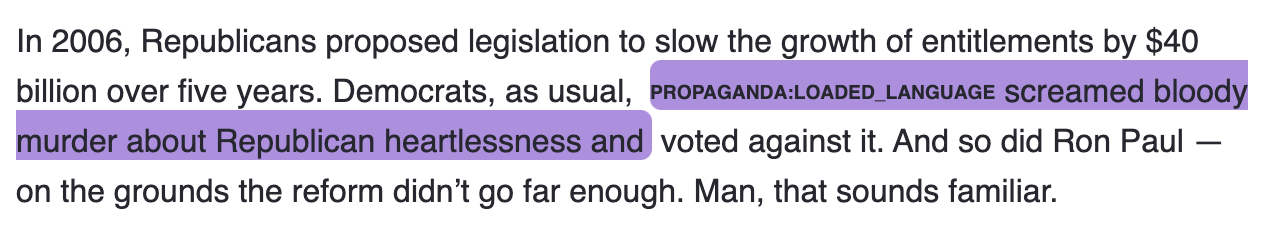
\includegraphics[width=\linewidth]{figures/propaganda_example_2.png}}
    \vspace{-20px}
    \caption{Example of a propaganda technique surrounded by multiple entities.}
    \vspace{-8px}
    \label{fig:propaganda_example_2}
\end{figure}

%\paragraph{Machine Learning Models}: In this paper, we pinned our analysis on neural network models. The additional features we calculated (e.g. TF-IDF, propaganda techniques) were added to NN models. This choice is influenced by the leading performance of such models in similar works. However, for completeness, we plan  to further test our propaganda-based features using other simpler machine learning models. %\textcolor{red}{Martino, check this plz} 

%\paragraph{Context}: %features considered do not have awareness of the context.
%Articles from different political sides about the same event will naturally overlap in terminology given the shared underlining story and context. 


%Figure~\ref{fig:propaganda_example_2} shows a sentence annotation from NationalReview in which the \texttt{Loaded\_Language} propaganda technique used: ``screamed bloody murder about Republican heartlessness''. As readers, we can immediately recognise that this paragraph is pro-republican, also because there is some kind of mocking of the Democrats with the phrase ``as usual'' and the closing ``Man, that sounds familiar''.
%For recognising this automatically, similarly to what~\citet{chen2017opinion} does considering only positive vs negative sentiment, we need to mine for each entity how it has been depicted by L/C/R.
% The feature vector for every entity shows how much propaganda techniques are used together with the entity.
% For example we could learn that Right-leaning sources have the entity ``Democratic Party'' occur in sentences where loaded language is used.
%Figure~\ref{fig:propaganda_example_2} is at the same time problematic because both Democratic and Republican co-occur with loaded language (and negative sentiment).
%An improvement could be done by considering that ``Democrats'' and ``Republican'' have a different role in the sentence (subject vs object of the propaganda technique).


% This entity-specific propaganda analysis would also enable %provide interpretability of the outputs. For example, this article is from the left because it uses propaganda technique X with entity Y, which is a usual thing for articles leaning left.

% This can also be verified by comparing what has been learned with the usual position of Left and Right leaning against topics \url{https://en.wikipedia.org/wiki/Left-wing_politics}.

%%%%%%A possible problem of this approach that is not defended in the paper, is the choice of articles that have been annotated by experts. They have been selected from sources "propagandistic by Media Bias/Fact Check", in other words from the page \url{https://mediabiasfactcheck.com/fake-news/}. The propagandistic sources listed in this page, as Figure~\ref{fig:mbfc_leaning} shows, are mostly on the extreme-right side of the spectrum. Furthermore, the selection done by the authors (table 3 of that paper) results in all the sources of the articles to lean on the right.
%So the resulting model is \textbf{being trained on very propagandistic sources from the right only}. The model will not be able to see left-propaganda because it never saw it in the training phase.

\subsection{Conclusions}
\label{ssec:ps_prop_leaning_classifier_conclusion}

This experiment analysed the relationship between propaganda and political leaning detection. Using available works for propaganda detection and political leaning, we explored the effects of the propaganda features on the task of political leaning classification. We showed that %(a) propaganda is found in Left, Centre, and Right leaning articles, 
(a) detecting political-leanings with propaganda features is challenging, and (b) detection performance improves when we combine the propaganda features with baseline features (\texttt{baly} dataset: amount of each propaganda technique together with the baseline features \texttt{(0)+(2)}, \texttt{NELA} dataset: \texttt{(0)+(1)+(2)} in most of the splits).

%produced negative to mixed results. However, it also showed a small positive impact on automated political-leaning classification of articles. 

% future
The appearance of propaganda, and the techniques used, showed not to be sufficient by themselves to boost the detection of political leaning.
The improvements observed are statistically significant, but they are very limited.
In the next Chapter~\ref{chap:topics}, we are going to focus on studying the effect of propaganda features in a more contextualised approach, by taking into account the topics and the relationship between propaganda and topics.
%, semantic entities, and authoring country. %observing the co-occurrence of propaganda with topics and entities, and from different geographic locations. This could help in recognising the main differences is use of propaganda in relation to article topics, authoring countries, and .
% This direction is supported by observing that many times the terms of propaganda from one side overlap with the terms from the other sides, so we want to capture in this way more context around the usage of the propaganda technique.








\section{\statusgreen Imbalance of Propaganda Datasets}
\label{ssec:ps_prop_leaning_imbalanced}

% exp 8: propaganda datasets are imbalanced

% motivation
% By seeing the results of the two previous experiments, we
In this section, we analyse whether the datasets, used for training propaganda recognition models, are balanced or not across political leaning.




% Orientation: Importance of propaganda computational studies
Over the last decades, several works have started addressing the recognition of propaganda techniques in text. As we have seen, a lot of progress has been done recently, from the detection of propaganda at the document-level to fine-grained technique analysis. The literature on computational detection of propaganda is quite recent~\citep{da2020survey}.
%But there is a limitation of these computational studies: they target just a subset of the propaganda, specifically the one from the extreme-right.
With the best of our knowledge, there is no current study of how balanced or imbalanced the propaganda datasets are across political leaning.




% RATIONALE
%Therefore, we want to address a gap between the historical socio-political works about populism, which find populism all over the political spectrum, and the computational studies to detect propaganda, which seem to have a much narrower view in the current situation.
%While it is common knowledge ??? that propaganda appears in different socio-political contexts, the computational approaches and datasets available currently have a narrower view.
% This view is currently linked to extreme-right leaning news sources, at the border with misinformation
% This view is linked to the US context of recent years and therefore it’s manifesting in the link between propaganda and far-right ideology (JUSTIFY THIS).

% Aim
Therefore, we want to study how the current datasets of propaganda are distributed across political leaning, and see if there is some imbalance in the datasets.
%
% Our aim is to analyse how observe how propaganda actually exists all over the political spectrum: not only in far-right media, but also in other leanings: left and also more moderate news sources use propaganda as a persuasion technique.
% And also to 
%
The research question that we aim to answer in this section is RQ3.3: \emph{How balanced are the current propaganda detection methods with regard to political leaning?}

% We analyse several propaganda detection datasets to understand the existing imbalance.



% In order to answer this additional question, we find that we need to rely\todoHA{how youo found this?} on the external concept of \gls{populism}, and therefore we also need to analyse \emph{How strongly is propaganda related to populism}.




% \todo{take key concepts from here, place them in the introduction below and remove this with the heading of "introduction"}

% Idea: from the propaganda detection tool, we saw that the data it’s trained on considers propaganda mainly from Right-leaning sources. But propaganda is common in every political leaning (literature) and also our experiment detected propaganda from every leaning. So we want to explore this gap between socio-political works (where propaganda is described as coming from every political leaning) and computational detection of propaganda (only targeted at recognising right-leaning).

% We have one hypotheses:
% \begin{itemize}
%     \item[H1:] propaganda exists all across the political spectrum;

% \end{itemize}
% \todoAW{Again, your terminology is a bit awry... I think you want to say that your null hypothesis (H0) is that propaganda exists across the spectrum and th alternative hypothesis is that propaganda co-0ccurs with populism.}



% Our narrative for this section proceeds with the following points:

% \begin{enumerate}
%     \item This goes against H1.
%     \item TODO link to appendix
%     \item Reflections: we sum up and discuss the discoveries of this analysis.
% \end{enumerate}

% Each of these steps is described in one of the following subsections. % contains one of these steps.

% \subsubsection{Introduction}

% % Orientation: Importance of propaganda computational studies
% Over the last decades, several works have started addressing the recognition of propaganda techniques in text. A lot of progress has been done already, from the detection of propaganda at the document level to fine-grained technique analysis. But there is a limitation of these computational studies: they target just a subset of the propaganda, specifically the one from the extreme-right. %(based on the US context).

% Propaganda is strongly linked to argumentation and rhetorics, it's the art of persuading listeners. And it has always been used by the state, media and political figures as a tool to convince the audience.

% Propaganda can be seen also from a different perspective, as a manipulation tool. For this reason, many studies (CITE) study propaganda together with fake news, misinformation, and hoaxes. However propaganda does not imply false content, but it’s something that is more on the edge of sensationalistic and strong language (spinned language, exaggeration, …).



% % RATIONALE
% Therefore, we want to address a gap between the historical socio-political works about propaganda, which find propaganda and populism all over the political spectrum, and the computational studies to detect propaganda, which seem to have a much narrower view in the current situation.
% While it is common knowledge that propaganda appears in different socio-political contexts, the computational approaches and datasets available currently have a narrower view.
% This view is currently linked to extreme-right leaning news sources, at the border with misinformation
% This view is linked to the US context of recent years and therefore it’s manifesting in the link between propaganda and far-right ideology (JUSTIFY THIS).


% % Aim
% Our aim is to observe how propaganda actually exists all over the political spectrum: not only in far-right media, but also in other leanings: left and also more moderate news sources use propaganda as a persuasion technique.

% % RQ
% The Research Question RQ3.3 is \emph{How balanced are the current propaganda detection methods with regard to political leaning?}
% are the following:

% (Why is computational research targeted against right-leaning propaganda? Is it a matter of quantity/context?) → related works
% Can we detect propaganda also in left and centre leanings? With a tool that is trained on right-leaning propaganda?
% How different is the detected propaganda across the political spectrum?

% RQ3.3.1: How different is the detected propaganda across the political spectrum? --> already answered in 5.3.1
% RQ3.3.2: Which generalisation problems can arise when applying a propaganda detection tool outside the usually-targeted extreme-right leaning?



% % Method
% 1. statistically it is all across
% 2. automatic classification of leaning based on propaganda features is not very good

% --> there should be some problems in the propaganda features

% For our experiment we use a propaganda annotation tool which tells the single detected words and the specific techniques used. By having this fine-grained analysis, we can do a quantity and term analysis across external dimensions, such as political leaning in this case.

% Then we try to find what distinguishes propaganda across the spectrum:
% - statistically: looking at quantities, terms ??? across the spectrum
% - by using a classifier and using propaganda features to predict the leaning


% Findings
% We find that, although the tool used is only trained on extreme right-leaning propagandistic
% articles, we can actually detect propaganda all across the spectrum. This ongoing experiment is directed at understanding the relationship between propaganda, points of view and the topics discussed

% We find that:
% - propaganda is almost evenly distributed across political spectrum
% - it is very difficult to differentiate whose propaganda it is, without having an explicit context representation (?????? We would need to find that representation and demonstrate that it works with the classifier ??????)

% Interpretation
% This means that we need more diversity of propaganda examples in order to be more generic than the specific US-based propaganda.



% \subsection{\statusgreen Corpora for propaganda detection: (im)balance analysis}
% \label{ssec:ps_prop_leaning_imbalanced_datasets}

We take a look at the available datasets of annotated instances of propaganda.
Our goal is to find if there are some overall trends, for example a big imbalance considering the political leaning.
% underline that most of the data belongs to right-leaning sources (extreme, not moderate).
% The gap is that the extreme left is usually not considered.

Note that the datasets that we consider are not the the ones used for political leaning that have been described in the previous Section~\ref{ssec:ps_leaning_data}.
% \todoHA{So why are we using them here?}
This is the case because we are analysing the task of propaganda detection and not the task of political leaning classification and, as we have seen in Chapter~\ref{chap:literature}, the literature is quite well separated between the two tasks.
We introduced propaganda in the previous chapter~\ref{chap:linguistic_persuasion}, but at that moment we had not yet introduced leanings into the analysis.
We present here the analysis of the propaganda detection datasets, showing how they distribute across political leanings.

% TSHP-17, QProp and PTC are mentioned in \citet{da2020survey}.


\subsection{TSHP-17}

%https://aclanthology.org/D17-1317.pdf dataset description: https://hrashkin.github.io/factcheck.html
The first dataset is TSHP-17, which was published in the work of~\citet{rashkin2017truth}. In this dataset, the articles are annotated accordingly to the news source that published them. Each news source belongs to a specific category:
\begin{itemize}
    \item Satire: The Onion, Borowitz Report, Clickhole
    \item Hoax: American News, DC Gazette
    \item Propaganda: Natural News, Activist Report (Activist News and Activist Report)
    \item Trusted news: from Gigaword News corups. Articles come from several sources, including AFP (Agence France Press), Associated Press, New York Times, The Xinhua News Agency. The dataset is not including these articles.
\end{itemize}

\begin{table}[!htbp]
    \centering
    \begin{tabular}{c|c|r|c|c}
        label                       & source               & \#articles & MBFC leaning  & MBFC link                                                                        \\
        \hline
        \multirow{3}{*}{satire}     & The Onion            & 14,170     & ?             & \href{https://mediabiasfactcheck.com/the-onion/}{the-onion}                      \\
                                    & The Borrowitz Report & 627        & left          & \href{https://mediabiasfactcheck.com/borowitz-report/}{borowitz-report}          \\
                                    & Clickhole            & 188        & ?             & \href{https://mediabiasfactcheck.com/clickhole/}{clickhole}                      \\
        \hline
        \multirow{2}{*}{hoax}       & American News        & 6,914      & extreme right & \href{https://mediabiasfactcheck.com/anews-24-com-american-news/}{american-news} \\
                                    & DC Gazette           & 5,133      & extreme right & \href{https://mediabiasfactcheck.com/dc-gazette/}{dc-gazette}                    \\
        \hline
        \multirow{2}{*}{propaganda} & Natural News         & 15,580     & far right     & \href{https://mediabiasfactcheck.com/natural-news/}{natural-news}                \\
                                    & Activist Report      & 17,869     & left          & \href{https://mediabiasfactcheck.com/activist-post/}{activist-post}              \\
        \hline
        trusted news                & Gigaword News        & 13.995     & ?             &
        % \multirow{}{*}{trusted news} & Natural News & 15,580 & far right & \href{https://mediabiasfactcheck.com/natural-news/}{natural-news} \\
        %                         & Activist Report & 17,869 & far left & \href{https://mediabiasfactcheck.com/activist-post/}{activist-post} \\
    \end{tabular}
    \caption{TSHP-17 dataset analysis across leaning.}
    \label{tab:tshp17_across_leaning}
\end{table}


% The other categories in the dataset are:
% Satire:
% The Onion:?  https://mediabiasfactcheck.com/the-onion/ 
% Borowitz Report: left-satire https://mediabiasfactcheck.com/borowitz-report/ 
% Clickhole: ? https://mediabiasfactcheck.com/clickhole/ 
% Hoax:
% American News: extreme-right https://mediabiasfactcheck.com/anews-24-com-american-news/ 
% DC Gazette: extreme-right https://mediabiasfactcheck.com/dc-gazette/ 
% Trusted news: from English Gigaword corpus:
% Agence France Press English Service: least biased https://mediabiasfactcheck.com/afp-agence-france-presse/ 
% Associated Press Worldstream English Service: left-center https://mediabiasfactcheck.com/associated-press/ 
% The New York Times Newswire Service: left-center https://mediabiasfactcheck.com/new-york-times/ 
% The Xinhua News Agency English Service: left https://mediabiasfactcheck.com/xinhua-news-agency/ 


% imbalance analysis
% Propaganda sources → quite balanced
% Hoax: mainly extreme-right
% Trusted news: left-center
We can see in Table~\ref{tab:tshp17_across_leaning} that the propaganda sources are quite balanced for this dataset, as we have one source that is labelled as ``far right" and one as ``left".
% may be one of the only
This dataset includes propaganda from both political-leanings and therefore we consider it as balanced. However, it is not annotated at the technique-level but only at the source level.


\subsection{QPROP Corpus}

This second dataset~\citep{alberto_barron_cedeno_2019_3271522}, comes from the work of~\citet{barron2019proppy}, and also in this case we have a collection of articles coming from a set of sources. These sources have source-level annotations coming from MBFC, from which the authors selected the two classes: \emph{propaganda} and \emph{trustworthy}.
For the \textit{trustworty} class we only know that they come from 94 sources with different leanings (left, left-center, center, right-center, right) and that in total there are 45.6k articles.
For the propaganda class instead, we have the breakdown of the sources considered, that is shown in Table~\ref{tab:qprop_across_leaning}.

% taken from MBFC data. http://proppy.qcri.org/about.html bad gateway (found on webarchive)
% https://zenodo.org/record/3271522\#.XS6qRUUzau4 
% Document-level annotations of propaganda

% Table 6 from paper, expanded with leaning and MBFC link

\begin{table}[!htbp]
    \centering
    \resizebox{\textwidth}{!}{
        \begin{tabular}{c|r|c|c}
            source                    & \#articles & MBFC leaning                        & MBFC link                                                                         \\
            \hline
            freedomoutpost.com        & 1,638      & ?                                   & \href{https://mediabiasfactcheck.com/freedom-outpost/}{freedom-outpost}           \\
            frontpagemag.com          & 1,259      & extreme right                       & \href{https://mediabiasfactcheck.com/frontpage-magazine/}{frontpage-magazine}     \\
            lewrockwell.com           & 821        & extreme right                       & \href{https://mediabiasfactcheck.com/lew-rockwell/}{lew-rockwell}                 \\
            shtfplan.com              & 778        & extreme right                       & \href{https://mediabiasfactcheck.com/shtfplan-com/}{shtfplan-com}                 \\
            vdare.com                 & 468        & extreme right                       & \href{https://mediabiasfactcheck.com/vdare/}{vdare}                               \\
            personalliberty.com       & 434        & extreme right                       & \href{https://mediabiasfactcheck.com/personal-liberty/}{personal-liberty}         \\
            remnantnewspaper.com      & 139        & extreme right                       & \href{https://mediabiasfactcheck.com/the-remnant-magazine/}{the-remnant-magazine} \\
            thewashingtonstandard.com & 115        & ?                                   &                                                                                   \\
            breaking911.com           & 73         & ? (82\%~MBFC viewers rate it~Right) & \href{https://mediabiasfactcheck.com/breaking911/}{breaking911}                   \\
            clashdaily.com            & 12         & extreme right                       & \href{https://mediabiasfactcheck.com/clash-daily/}{clash-daily}                   \\
        \end{tabular}
    }
    \caption{QPROP dataset analysis across leaning.}
    \label{tab:qprop_across_leaning}
\end{table}

% imbalance analysis
We can see that all the sources, with the exception of three of them (two without leaning annotation, and one with only the votes from MBFC viewers), are rated as having a \emph{extreme right} leaning.
% Apart from 3 sources (not found/unknown bias), they are all extreme right sources.

\subsection{PTC Corpus}
This dataset comes from another work by the same research group as the previous QPROP.
With respect to the previous datasets, this one has fine-grained annotations of the specific propaganda techniques. The dataset is presented in~\citet{da2019fine}, that is also our reference for our experiments from Chapter~\ref{ssec:lp_techniques_propaganda} and is the one that differentiates between 18 different propaganda techniques.
Table~\ref{tab:ptc_across_leaning} shows the sources that were used to build this dataset. We can notice that most of the sources are the same as in the previous QPROP. But this time the number of articles is much smaller because the annotations have been performed with much higher granularity (not at the source-level but at the technique-level with specific words annotated).
% is the one from Da San Martino 2019 https://aclanthology.org/D19-1565.pdf that the tool is trained on.
% Annotation guidelines: https://aclanthology.org/D19-1565/ (in the attachment)
% Definition of the techniques: https://propaganda.qcri.org/annotations/definitions.html 
% Fine-grained techniques

\begin{table}[!htbp]
    \centering
    \resizebox{\textwidth}{!}{
        \begin{tabular}{c|r|c|c}
            source                    & \#articles & MBFC leaning                        & MBFC link                                                                         \\
            \hline
            freedomoutpost.com        & 133        & ?                                   & \href{https://mediabiasfactcheck.com/freedom-outpost/}{freedom-outpost}           \\
            frontpagemag.com          & 56         & extreme right                       & \href{https://mediabiasfactcheck.com/frontpage-magazine/}{frontpage-magazine}     \\
            shtfplan.com              & 55         & extreme right                       & \href{https://mediabiasfactcheck.com/shtfplan-com/}{shtfplan-com}                 \\
            lewrockwell.com           & 26         & extreme right                       & \href{https://mediabiasfactcheck.com/lew-rockwell/}{lew-rockwell}                 \\
            vdare.com                 & 20         & extreme right                       & \href{https://mediabiasfactcheck.com/vdare/}{vdare}                               \\
            remnantnewspaper.com      & 19         & extreme right                       & \href{https://mediabiasfactcheck.com/the-remnant-magazine/}{the-remnant-magazine} \\
            personalliberty.com       & 18         & extreme right                       & \href{https://mediabiasfactcheck.com/personal-liberty/}{personal-liberty}         \\
            Remnant Magazine          & 14         & extreme right                       & \href{https://mediabiasfactcheck.com/the-remnant-magazine/}{the-remnant-magazine} \\
            breaking911.com           & 11         & ? (82\%~MBFC viewers rate it~Right) & \href{https://mediabiasfactcheck.com/breaking911/}{breaking911}                   \\
            truthuncensored.net       & 8          & extreme right                       & \href{https://mediabiasfactcheck.com/truth-uncensored/}{truth-uncensored}         \\
            thewashingtonstandard.com & 6          & ?                                   &                                                                                   \\
            www.unz.com               & 5          & extreme right                       & \href{https://mediabiasfactcheck.com/the-unz-report/}{the-unz-report}             \\
            clashdaily.com            & 1          & extreme right                       & \href{https://mediabiasfactcheck.com/clash-daily/}{clash-daily}                   \\
        \end{tabular}
    }
    \caption{PTC dataset analysis across leaning.}
    \label{tab:ptc_across_leaning}
\end{table}

% imbalance analysis
This dataset suffers, as the previous one, of a high imbalance of the leaning of the sources included.
% Apart from 3 sources (not found/unknown bias), they are all extreme right sources. (sources very similar to the ones from QPROP, the dataset is from the same research group)

\subsection{Media Bias/Fact Check propaganda}
As both the previous QPROP and PTC are derived from a subset of MBFC propaganda sources, we analysed the full MBFC propaganda subset.

“Propagandist sources” (also selected from here for Qprop and PTC), are listed in the MBFC under the name ``questionable sources".\footnote{\url{https://mediabiasfactcheck.com/fake-news/}}
We retrieved the details of these sources, and discovered that 85\% of the sources that have ``propaganda" in the label are from the Right.

\begin{figure}[!htbp]
    \centering
    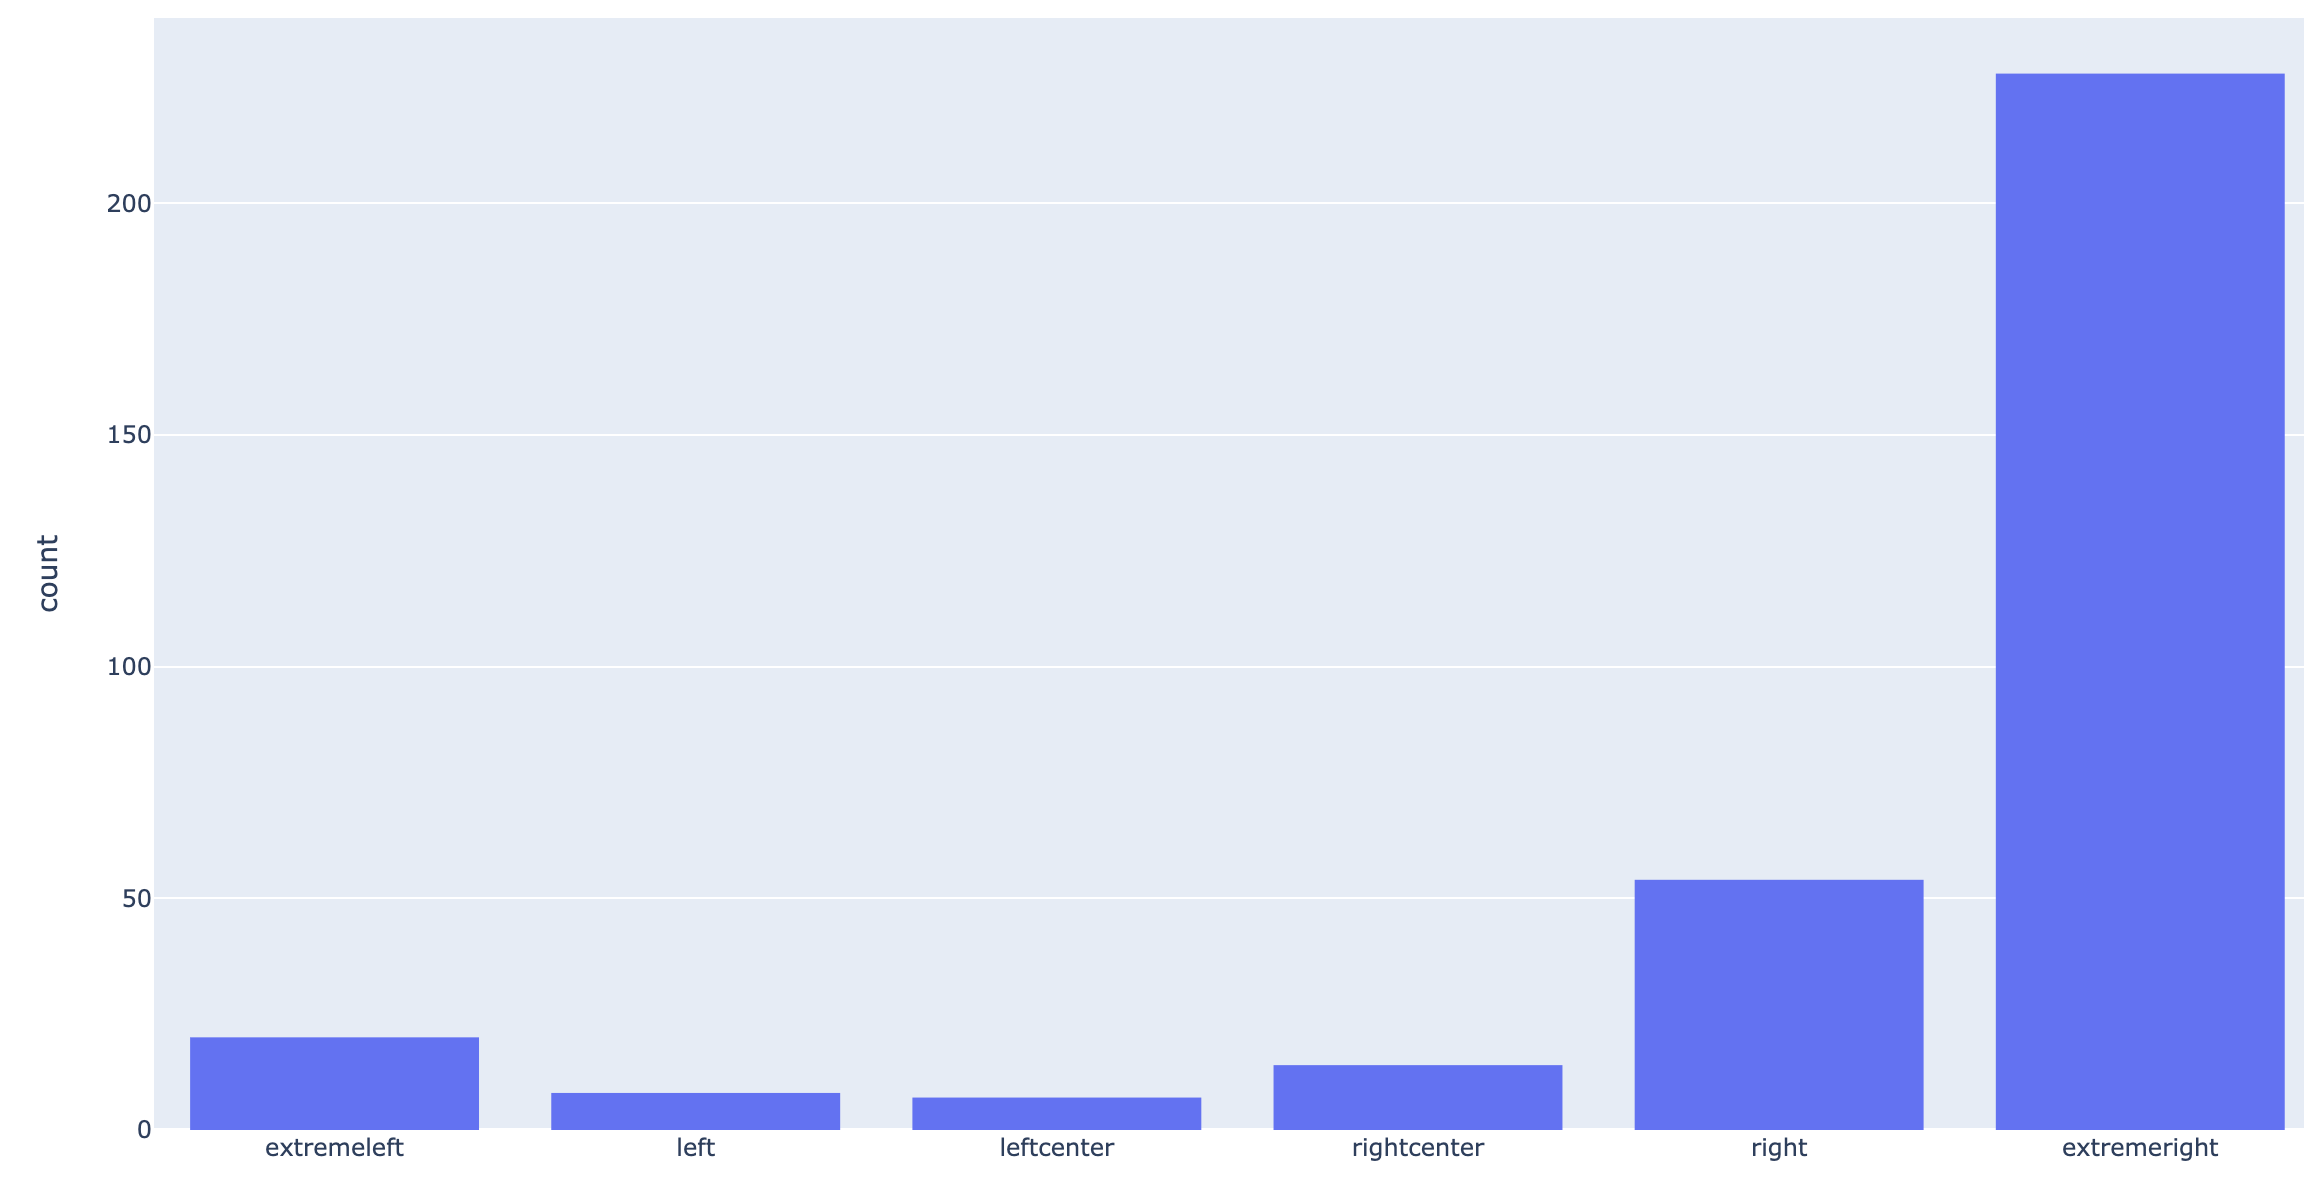
\includegraphics[width=\linewidth]{figures/leaning_questionable.png}
    \caption{MBFC dataset analysis: sources across leaning.}
    \label{fig:mbfc_across_leaning}
\end{figure}

% imbalance analysis
% Most of the propagandist sources are from the right. But at the same time, PTC and QPROP selected only from the right. Ignoring the 15% from left/center.
As we can see in Figure~\ref{fig:mbfc_across_leaning}, this dataset is very imbalanced. But what is even more imbalanced, is the selection that was done by the creators of PTC and QPROP, completely excluding left-leaning and center sources (15\% totally underrepresented).

% - Possible problems?
% A possible problem of this approach %that is not defended in the paper, 
% is the choice of articles that have been annotated by experts. They have been selected from sources "propagandistic by Media Bias/Fact Check", in other words from the page \url{https://mediabiasfactcheck.com/fake-news/}. The propagandistic sources listed in this page, as Figure~\ref{fig:mbfc_leaning} shows, are mostly on the extreme-right side of the spectrum. Furthermore, the selection done by the authors (table 3 of that paper) results in all the sources of the articles to lean on the right.
So the resulting models that use these imbalanced datasets, are \textbf{being trained on very propagandistic sources from the right only}. The models may have some problems in detecting correctly left-leaning propaganda because they never saw it in the training phase. This may manifest in different expressions or even different techniques, that become very difficult to detect with an imbalanced training.

% Most of them are from the far-right, but these are from Left (also there were some from the center)x2:
% https://mediabiasfactcheck.com/basnews-agency/
% https://mediabiasfactcheck.com/bbarta24/
% https://mediabiasfactcheck.com/bdnews24/ 
% https://mediabiasfactcheck.com/beijing-review/
% https://mediabiasfactcheck.com/bipartisan-report/
% https://mediabiasfactcheck.com/blacknews-com/
% https://mediabiasfactcheck.com/bossip/
% https://mediabiasfactcheck.com/cctv-america/
% https://mediabiasfactcheck.com/true-activist/
% https://mediabiasfactcheck.com/china-daily/
% https://mediabiasfactcheck.com/china-global-television-network-cgtn/



% Most of the sources that have “Propaganda” are from the right: 85\%

% Propaganda vs the other labels listed as “questionable reasoning”

% \paragraph{Media Bias/Fact Check propaganda intersection with Baly}
% MBFC propagandistic sources intersected with Baly sources:
% {'breitbart.com',  'theepochtimes.com',  'newsmax.com',  'townhall.com',  'dailymail.co.uk',  'theblaze.com'} → all right / extreme-right

% \paragraph{Media Bias/Fact Check propaganda intersection with NELA}
% MBFC propagandistic sources intersected with NELA sources:
% {'conservative tribune', 'daily stormer', 'western journal', 'newswars', 'freedom daily', 'true activist', 'the duran', 'the d.c. clothesline', 'breitbart', 'bipartisan report', 'the right scoop', 'dc gazette', 'frontpage magazine', 'the gateway pundit', 'cns news', 'daily mail'} 
% From Left-leaning:
% {'true activist', 'bipartisan report'} → from Left:
% True Activist https://mediabiasfactcheck.com/true-activist/ : 370 articles in NELA
% Bipartisan Report: 4060 articles in NELA

\subsection{In Other Languages}

We also analysed other datasets of propaganda that we found occurring for other languages, to see if this imbalance also exists in other countries and languages.


% https://www.mdpi.com/2306-5729/7/3/29/htm 
% https://zenodo.org/record/5828240\#.YduLv2hBxPY 
First of all, we find two datasets in Hindi: \textbf{H-Prop} and \textbf{H-Prop-News}~\citep{chaudhari2022h,chaudhari_deptii_2022_5828240}.
The first one, \textbf{H-Prop}, is the translation of a subset of QPROP. The authors translated 28k articles (out of 51k total) with IBM Watson, and built this dataset. It has the same features as QPROP, and given that QPROP had no articles coming from the Left or Center, H-Prop also does not. The data, therefore, is still imbalanced.

H-Prop-News instead is scraped from 30+ prominent Hindi News websites. The labeling was done by human annotators and the inter-annotator agreement using Cohen’s Kappa is 0.81.

\begin{table}[!htbp]
    \centering
    \resizebox{\textwidth}{!}{
        \begin{tabular}{c|r|r|P{0.23\textwidth}|c}
            source          & \#non-prop articles & \#prop articles & MBFC leaning                                                                                           & MBFC link                                                                                        \\
            \hline
            Amar Ujala      & 360                 & 244             & \multirow{3}{=}{\setlength\parskip{\baselineskip}Right? in the top 4 controlling Indian media (right)} & \multirow{3}{*}{\href{https://mediabiasfactcheck.com/india-media-profile/}{india-media-profile}} \\
            Bhaskar         & 293                 & 204             &                                                                                                        &                                                                                                  \\
            Dainik Jagran   & 269                 & 238             &                                                                                                        &                                                                                                  \\
            \hline
            One India       & 166                 & 120             & Left-center                                                                                            & \href{https://mediabiasfactcheck.com/oneindia/}{oneindia}                                        \\
            Zee News        & 150                 & 85              & ?                                                                                                      &                                                                                                  \\
            Patrika         & 133                 & 347             & ?                                                                                                      &                                                                                                  \\
            News On AIR     & 131                 & 20              & ?                                                                                                      &                                                                                                  \\
            India           & 130                 & 78              & right-center                                                                                           & \href{https://mediabiasfactcheck.com/india-com/}{india-com}                                      \\
            Punjab Kesari   & 121                 & 78              & ?                                                                                                      &                                                                                                  \\
            Dainik Tribune  & 114                 & 79              & ?                                                                                                      &                                                                                                  \\
            Khas Khabar     & 111                 & 63              & ?                                                                                                      &                                                                                                  \\
            TV9 Hindi       & 111                 & 99              & ?                                                                                                      &                                                                                                  \\
            Samay Live      & 107                 & 111             & ?                                                                                                      &                                                                                                  \\
            Lokmat News     & 95                  & 52              & ?                                                                                                      &                                                                                                  \\
            Tehelka Hindi   & 77                  & 156             & ?                                                                                                      &                                                                                                  \\
            ABP Live        & 76                  & 40              & ?                                                                                                      &                                                                                                  \\
            Dainik Navjyoti & 78                  & 56              & ?                                                                                                      &                                                                                                  \\
            Pratahkal       & 63                  & 85              & ?                                                                                                      &                                                                                                  \\
            Jansatta        & 61                  & 93              & ?                                                                                                      &                                                                                                  \\
            Asianet News    & 51                  & 21              & ?                                                                                                      &                                                                                                  \\
            BBC Hindi       & 36                  & 21              & ?                                                                                                      &                                                                                                  \\
            Nai Duniya      & 32                  & 15              & ?                                                                                                      &                                                                                                  \\
            Oulook Hindi    & 25                  & 54              & ?                                                                                                      &                                                                                                  \\
            Univarta        & 16                  & 3               & ?                                                                                                      &                                                                                                  \\
            The Quint       & 15                  & 28              & left-center                                                                                            & \href{https://mediabiasfactcheck.com/the-quint/}{the-quint}                                      \\
            Bebak Post      & 12                  & 16              & ?                                                                                                      &                                                                                                  \\
            The Wire        & 12                  & 34              & left-center                                                                                            & \href{https://mediabiasfactcheck.com/the-wire-india/}{the-wire-india}                            \\
            Live Hindustan  & 11                  & 8               & ?                                                                                                      &                                                                                                  \\
            Aaj Tak         & 10                  & 168             & ?                                                                                                      &                                                                                                  \\
            DW              & 9                   & 1               & ?                                                                                                      &                                                                                                  \\
            Times Now       & 5                   & 8               & ?                                                                                                      &                                                                                                  \\
            India TV        & 0                   & 5               & right-center                                                                                           & \href{https://mediabiasfactcheck.com/india-tv/}{india-tv}                                        \\
        \end{tabular}
    }
    \caption{H-Prop-News dataset analysis across leaning.}
    \label{tab:hpropnews_across_leaning}
\end{table}

% imbalance analysis
We can see in Table~\ref{tab:hpropnews_across_leaning}, that the labelling did not occur at the source level, but at the article level. In fact, for each source there are both propagandistic and non-propagandistic articles.
For the leaning, we see that for most of the sources we do not have enough information, as MBFC, AllSides and AdFontesMedia do not provide informationo about them. But from the few data points available, this dataset looks more balanced in terms of leaning.


% Czech Newspaper texts Propaganda
The next dataset that we found in other languages is published in~\citet{baisa2019benchmark}.
% Data not published online
The dataset is composed of news articless coming from four news sources: sputnik.cz, parlamentnilisty.cz, ac24.cz and www.svetkolemnas.info. For these four sources, we could only find some information about Sputnik which is annotated as \href{https://mediabiasfactcheck.com/sputnik-news/}{right-center from MBFC}.
% imbalance analysis
So it becomes difficult to understand if there is some imbalance or not.
This dataset contains also fine-grained annotations of the techniques, and they are contextualised to the situation in Czech Republic.
% As anotherList of techniques is different from Di Martino 2019, interesting
% 1 source out of 4 is from right, the others are unknown. So it may be imbalanced?

We also found other datasets related to China or to the Russo-Ukrainian conflict, but they do not contain information about the political leaning so we had to discard them from our analysis.

% \paragraph{Other corpora (not news)}
% For this set of datasets, no leaning information is available, so it’s impossible to analyse the imbalance
% PRC tweets with propaganda in china
% https://arxiv.org/pdf/2106.07544.pdf
% https://github.com/annabechang/Propaganda\_Tech\_Twitter\_PRC 
% No info on leaning, but they chose the same techniques as in Da San Martino 2019. Manual annotators (2 for each tweet)
% Reddit pro-China vs neutral
% https://arxiv.org/pdf/2108.12269.pdf 
% No data public?
% Russia-Ukraine tweets
% https://arxiv.org/pdf/2203.02955.pdf 
% Data: https://github.com/ehsanulhaq1/russo\_ukraine\_dataset 
% No explicit encoding of propaganda, it’s just a collection of tweets related to a list of keywords/mentions, so this dataset is not useful
% PropaNews
% https://arxiv.org/pdf/2203.05386.pdf
% Data not yet published (paper from March 2022)
% Data contains generated articles that are loaded with propaganda techniques. Keep an eye on this if released
% Russia-ukraine VK
% https://www.kaggle.com/datasets/ustyk5/war-in-ukraine-russian-social-network-discussions 
% It’s in russian. Open challenge for Kaggle community
% Russian propaganda from EuVsDisinfo
% https://www.kaggle.com/datasets/stevenpeutz/misinformation-fake-news-text-dataset-79k?select=EXTRA\_RussianPropagandaSubset.csv 
% This file “EXTRA” contains data from EuVsDisinfo and is labelled as misinformation/propaganda (not distinguished).

\subsection{Overall Trend}
From this view on the computational detection resources, we recognise a quite strong skew over right-leaning sources that is happening in the English-based datasets.
The main reason is that the corpora are based on the already-imbalanced MBFC propaganda collection. The imbalance is pushed even more during the sampling of news sources, resulting in datasets being completely imbalanced.
This happens especially for the PTC corpus, which is the only one that provides fine-grained annotation of techniques.
For other languages, we do not have enough information to draw conclusions.
% \todoHAinline{Exactly. So I'm struggling with this section and what to do with it.}

% This finding of imbalanced datasets clashes with our hypothesis H1.
Finding this imbalance in the data makes us question which of the two following cases we are in:

\begin{enumerate}
    \item Propaganda is mainly linked to Right-leaning. Although this relationship is not found in the literature anywhere, it might be the case. Being in this case would mean that Left-leaning would be less prone to use propaganda, and we find this highly improbable. We know from the literature that for example many slogans exist in the Left (e.g. ``Black Lives Matter", ``Defund the Police", ``Stronger, Safer and Better Off" (UK)) and slogans is only the easiest propaganda technique to think about. This case, therefore, is not very likely to be true.
    \item Propaganda is spread all around political leanings, as a mean of persuasion. Its different techniques may be used differently depending on the political orientation, but it is traversal to the political spectrum. In this case
          % H1 would be true, and 
          the problem of imbalance of the existing propaganda datasets becomes a real problem, with possible implications (not being able to detect accurately left-leaning propaganda).
\end{enumerate}

\subsection{Discussion}
% Appendix~\ref{app:prop_and_populism} where we analyse propaganda and populism
% \todo{properly link appendix to this discussion}
We analysed the imbalance of propaganda datasets, showing how the majority of them is derived from MBFC that is already imbalanced and during the sampling some categories of leanings disappear completely.

Finding that most of the datasets are focused on Right-leaning propaganda, the next logical question that comes to us is: \emph{Why would propaganda datasets/detection need to be more balanced across the political spectrum?} In other words, does propaganda exist from all political leanings?
I propaganda exists with all political leanings, this means that the detection resources (datasets) should contain examples across the spectrum in order to be able to recognise propaganda better.

This discussion, diverting slightly from the core goals of this thesis, is treated within Appendix~\ref{app:prop_and_populism}.
In the appendix we explain the conceptual relationship of populism and propaganda, we show that propaganda exists across all political contexts and leanings, and we also demonstrate how the imbalance of the considered propaganda detection is showing some inconsistencies (correlation between detected propaganda techniques and populism).





% (This was from discussion of what is now in appendix)

% Disclaimer: 
% We feel that at this point we need to state a disclaimer: we are interested of studying the propaganda detection and its unbalance independently by the goals that it is used for. 
\emph{Why} do we think that this imbalance needs to be corrected?
We are interested in detecting the techniques from text and how the imbalance that we found could result in lower detection accuracy.
We observe this imbalance and we want to make the readers of this thesis aware that the current propaganda datasets are imbalanced and they should be more inclusive.
We think that it is useful to detect all leanings of propaganda independently of one's own political ideology. %, and this work is not to be intended at any point as 
Propaganda may be used both for good and bad purposes. It is a set of persuasion techniques and this analysis of imbalance aims at providing directions to improve the detection.




% possible problems
% We want to understand if propaganda can be also detected on sources from the left and centre.
The resulting models that use these imbalanced datasets, are \textbf{being trained on very propagandistic sources from the right only}. The models may have some problems in detecting correctly left-leaning propaganda because they never saw it in the training phase. This may be caused by different expressions or even different techniques.

% Is this imbalance a problem? Are the propaganda techniques used by the left and the right actually different, or they are the same and the only thing that changes is the end goal of using propaganda?

% % Which generalisation problems can arise when applying a propaganda detection tool outside the usually-targeted extreme-right leaning?

% We currently can only leave these questions unanswered


\section{\statusgreen Discussions}
\label{sec:ps_discussions}

This chapter introduced the ingredient of Political Leaning that was analysed first on its own and then put in relationship with the previously analysed concepts of Persuasion and Propaganda.

Each of the three Research Questions has been analysed, and this is a reminder of the results obtained:

% reminder of the results
\begin{enumerate}[label={\textbf{RQ3.\arabic*:}},leftmargin=2cm]
    \item \emph{How does persuasion vary across the political spectrum?} We detect less propaganda in the centre and more in the extremes. This was already hypothesised since more extreme points of view have usually stronger opinions which reflect in the language they use. Between Left and Right, the Right seems to be more propagandistic, especially with some techniques (\texttt{Flag-Waving} and \texttt{Slogans}). With the term analysis, we are able to relate to some contextual elements and for example recognise some slogans and terminology of the Left and Right. We see that different political leanings seem to be quite recognisable by observing the comparison of quantities and terms. This motivates us to proceed with the next RQ.
    \item \emph{To what extent can we predict the political leaning of a news article by observing the propaganda it uses?} We experimented with a classifier trained with different combinations of features, and the result is that propaganda features cannot themselves reach the recognition abilities of the BERT baseline. When combined with the baseline features, we see in some cases some small improvements, that test as significant according to McNemar tests. In these cases, the propaganda features help to correct some imbalances of the baseline classifier. However, the number of samples affected is quite small. This may be because BERT is already a very powerful model and any improvements over it have to be considered as a win already.
    \item \emph{How balanced are the current propaganda detection methods with regard to political leaning?} We then performed an analysis of the imbalance of the main datasets that are used for the English language to perform propaganda detection. The results are clearly indicating that most of them are imbalanced. It is not very clear what the effect of this imbalance is, but we can already see some of its effects by analysing the correlation with populism. Indeed, we see that some detected propaganda techniques result in being negatively correlated with populism. In our opinion, this is an indicator that more studies are needed to establish whether our hypotheses are wrong or if propaganda detection is having some problems.
\end{enumerate}


We can then summarise an answer to our overall RQ3: \emph{To what extent could the use of persuasion techniques help identify the political leaning of a news article?}
We observed and used the potential of persuasion analysis (more specifically, propaganda detection) to recognise the political leaning of news articles. The results are promising but are undermined by a high imbalance in the datasets used for training propaganda detection models.



% What this means
These findings are quite meaningful for us.
% - positive: generalisation quite good considering datasets and results obtained
First of all, they show how current propaganda detection is able to work with articles coming from very different political orientations. We think that the results here found are demonstrating quite good abilities to generalise from the relatively small datasets used for training propaganda.
If we consider that a big proportion of the news used in our experiments comes from a different political leaning, we think that these are very promising results.
We were able to extract, analyse and link to our external knowledge of the events and ideologies. This is a very positive outcome.

% - finding TOPICS where difference is more accentuated
At the same time, this chapter has also helped us to find a direction for more investigation. The results found here represent the whole dataset. We would like to know if we can spot more in detail the differences of propaganda when we consider specific topics separately. Propaganda may differ between political leanings more when we select certain topics, and we would like to know both which topics and also the outcomes of such a detailed analysis. For conducting this experimentation, we need to consider the \emph{topics} of the articles as an additional element.

% limitation
Unfortunately, the experiment conducted also revealed possible limitations of automated fine-grained propaganda detection.
We have some observations that go against our hypotheses (e.g., some propaganda techniques in certain leanings, where we observed a negative correlation with populism), and we observed also on some samples some problems in detecting the edges of propaganda spans in the text.
These limitations come from a quite recent task (fine-grained detection of techniques) and indicate that more experimentation is needed. The current resources may be improved with more data annotated by humans, and the current findings need to be validated or confuted with more resources.

% finding TOPICS where propaganda works better/worse
While this is outside the scope of this thesis, we can instead practically contribute to finding where and how the detection of propaganda techniques is more problematic.
Adding the \emph{topics} into our analysis would also be beneficial in order to understand how propaganda detection performs across them.
We can try to identify the topics where there are possibly some problems and guide better the development of new resources about propaganda detection.


\section{\statusgreen Next}
\label{sec:ps_next}

We have two main motivations to drive the next experimental Chapter~\ref{chap:topics} into the analysis of the topics.

The first one, is to find in which topics propaganda varies mostly across the political spectrum. There may be some topics where the discussion is not using a lot of propaganda techniques to drive the reader in a certain direction, or where the usage may not be very distinctive (e.g., when talking about sports, Left and Right persuasion may be quite difficult to tell apart).
With an analysis of the topics, we can find the ones where the detected propaganda differs the most, and therefore where we can try to recognise automatically more easily the political leaning of a news article by using the propaganda features.
% Propaganda features are not enough to recognise leaning %, and propaganda seems to be spread around in almost all leanings.
% We need to find whether, by including another dimension, we can differentiate better. 
% Does it depend on the topics of the articles?
% Need to break down by topic and see whether for some of them, propaganda of one leaning is very different from the one of the others.

% Motivation 2
Another strong motivation to analyse the topics is to try to locate where the current approach to propaganda detection might have some issues in being accurate.
% Find topics where propaganda detection might have some problems
We will perform this analysis and try to find insights that could lead to the development of future propaganda detection resources (e.g., datasets) that are less subject to the imbalance problems that we found in this chapter.

% \todoHAinline{The section on populism seems redundant.}

% \todo{From meeting of 2 March 2023
% % Rather long.
% % Difficult to follow the structure (5.3.2.1 → NO).
% % “Significant”: only use when testing with p-value.
% “Hypothesis”: only use when H0 null hypothesis.
% % Hypothesis H1 and H2 (populism) in 5.3.3 bit confusing.
% Consistency of the structure: declare once methodology and structure and follow in all the experiments.
% A lot of technical details, not clear the goal.
% Each experiment should be standalone in a section, now table referring lots of pages after.
% Unbalance after tons of pages and experiments, only to say at the end that they are unbalanced → move around order of story != chronological order
% % Populism: what is it adding? What I want the reader to understand about it?
% Order of RQ: maybe move dataset imbalance before / another chapter?
% % LPT technique: justify more.
% This chapter has a lot of data and analysis but needs better narrative.
% Add examples: datasets, etc.
% % Word clouds: remove, waste of time of the examiner.
% % Heatmaps: to get something concrete is quite difficult, and if printed B/W they become impossible to read.
% Differentiate between what I did and what someone else did: no passive voice, check voice used.
% % Datasets: which ones have been used, which ones NOT?
% % Splits is very important part of the methodology.
% % Methodology should be all together (splits, models, steps, evaluation)
% % First worry about the structure, then about the size.
% % Reorganize chapter:
% % Create separated structure,
% % Cut and paste in the correct section the content.
% } 